\documentclass[a4paper,12 pt,twoside]{report}
\usepackage[utf8]{inputenc} 
\usepackage[T1]{fontenc}     
\usepackage[main = UKenglish,french]{babel}
\usepackage[top=2.4cm, bottom=2.4cm, left=1.4cm, right=1.4cm,headheight=14.5pt]{geometry}
%\usepackage[backend=bibtex]{biblatex}
%\bibliography{biblio.bib}

%	# Packages load

\usepackage[labelfont=bf,justification=centering]{caption}
% The cap­tion pack­age pro­vides many ways to cus­tomise the cap­tions in float­ing en­vi­ron­ments like fig­ure and ta­ble, and co­op­er­ates with many other pack­ages.
% url =  https://www.ctan.org/pkg/caption

\usepackage{amsmath}
% It adapts for use in LATEX most of the math­e­mat­i­cal fea­tures found in AMS-TEX; it is highly rec­om­mended as an ad­junct to se­ri­ous math­e­mat­i­cal type­set­ting in LATEX.
% url =  https://www.ctan.org/pkg/amsmath

\usepackage{amssymb}
% Provides an extended symbol collection.
% url =  ftp://ftp.dante.de/tex-archive/fonts/amsfonts/doc/amssymb.pdf

\usepackage{amsfonts}
% An ex­tended set of fonts for use in math­e­mat­ics.
% url =  https://www.ctan.org/pkg/amsfonts

\usepackage{enumitem}
% This pack­age pro­vides user con­trol over the lay­out of the three ba­sic list en­vi­ron­ments: enu­mer­ate, item­ize and de­scrip­tion.
% url =  https://www.ctan.org/pkg/enumitem

\usepackage{physics}
% The pack­age de­fines sim­ple and flex­i­ble macros for type­set­ting equa­tions in the lan­guages of vec­tor cal­cu­lus and lin­ear al­ge­bra, us­ing Dirac no­ta­tion.
% url =  https://www.ctan.org/pkg/physics

\usepackage{graphicx}
% The pack­age builds upon the graph­ics pack­age, pro­vid­ing a key-value in­ter­face for op­tional ar­gu­ments to the \in­clude­graph­ics com­mand.
% url =  https://www.ctan.org/pkg/graphicx

\usepackage{hyperref} 
% The hy­per­ref pack­age is used to han­dle cross-ref­er­enc­ing com­mands in LATEX to pro­duce hy­per­text links in the doc­u­ment.
% url =  https://www.ctan.org/pkg/hyperref
%\hypersetup{colorlinks=true, allcolors=blue}

\usepackage{fancyhdr} 
% The pack­age pro­vides ex­ten­sive fa­cil­i­ties, both for con­struct­ing head­ers and foot­ers, and for con­trol­ling their use
% url = https://www.ctan.org/pkg/fancyhdr

\usepackage{csquotes}
% This pack­age pro­vides ad­vanced fa­cil­i­ties for in­line and dis­play quo­ta­tions.
% url = https://www.ctan.org/pkg/csquotes

\usepackage{wrapfig}
% Al­lows fig­ures or ta­bles to have text wrapped around them.
% url =  https://www.ctan.org/pkg/wrapfig

\usepackage{subcaption}
% Permet de faire des sous-figures très facilement !

\usepackage{csquotes}
% Améliore les citations

\usepackage{indentfirst}
% Rajoute un alinéa tout le temps

% # Page style congiguration (fancyhdr)

\pagestyle{fancy}

\fancyhf{}% Clear header and footer
%\fancyhead[LE,RO]{\slshape  \rightmark}
%\fancyhead[LO,RE]{\leftmark}
\fancyfoot[C]{\thepage}% Custom footer
\renewcommand{\headrulewidth}{0pt}
\renewcommand{\footrulewidth}{0pt}

%\fancypagestyle{plain}
%{
%	\fancyhf{}%
%	\fancyfoot[C]{\thepage}%
%	\fancyhead[LE,RO]{\slshape  \rightmark}
%	\renewcommand{\headrulewidth}{0pt}
%}  

% # First page setup

\newcommand*{\titleGP}
{
	\begingroup % Create the command for including the title page in the document
	\newgeometry{top=1.4cm, bottom=0.8cm, left=1.4cm, right=1.4cm,headheight=14.5pt}
	\thispagestyle{empty}	
	\centering % Center all text
	\rule{\textwidth}{1.6pt}\vspace*{-\baselineskip}\vspace*{2pt} 
	\rule{\textwidth}{0.4pt}\\[\baselineskip] 
	\vspace*{-0.6\baselineskip}
	{\LARGE \textsc{Dynamics of a superfluid helium nanodroplet} \par} 
	\vspace*{0.2\baselineskip}
	{\LARGE \textsc{doped with a single potassium atom}}\\[0.15\baselineskip] % Title
	\rule{\textwidth}{0.4pt}\vspace*{-\baselineskip}\vspace{3.2pt} % Thin horizontal line
	\rule{\textwidth}{1.6pt}\\[\baselineskip] % Thick horizontal line
	\vfill
	\begin{figure}[h!]
		\centering
		\includegraphics[scale=0.35]{../pictures/couverture}
	\end{figure}	
	\vfill
	{\LARGE \textbf{Maxime \textsc{Martinez}$\,^{\circledast}$}\par} 
	\vspace*{0.1\baselineskip}
	{\large M2 \textit{Physique Fondamentale}, \textsc{Université Toulouse III Paul Sabatier}\par} 
	\vspace*{1.0\baselineskip}
	{\itshape Under the supervision of N.~\textsc{Halberstadt}$\,^{\circledast}$ and F.~\textsc{Coppens}$\,^{\circledast}$ \par}
	{\itshape In tight collaboration  with M.~\textsc{Barranco}$\,^{\circledast\circledcirc}$ and M.~\textsc{P\'i}$\,^{\circledcirc}$ \par}
	\vspace*{1.0\baselineskip}
	{\itshape \footnotesize $^{\circledast}$Laboratoire des Collisions, Agr\'egats, R\'eactivit\'e, IRSAMC, UMR 5589, CNRS et Universit\'e~Toulouse~III Paul~Sabatier, 118 route de Narbonne, Toulouse Cedex, France \par}
	\vspace*{0.1\baselineskip}
	{\itshape \footnotesize $^{\circledcirc}$Departament FQA, Facultat de F\'isica, and IN2UB, Universitat de Barcelona, Diagonal 645, 08028 Barcelona, Spain\par}
	\vspace*{-0.7\baselineskip}
	\begin{figure}[h!]
	\centering
	\begin{minipage}[c]{0.52\linewidth}
\centering
		
\includegraphics[scale=0.7]{../pictures/logo-UPS}
	\end{minipage}
\hfill
	\begin{minipage}[c]{0.44\linewidth}
\centering
		
\includegraphics[scale=0.9]{../pictures/logo-lcar}
	\end{minipage}
\end{figure}
	\restoregeometry
	\endgroup
}

\usepackage{tabularx}
\usepackage[explicit]{titlesec}

\usepackage{etoolbox}

\makeatletter
\patchcmd{\ttlh@hang}{\parindent\z@}{\parindent\z@\leavevmode}{}{}
\patchcmd{\ttlh@hang}{\noindent}{}{}{}
\makeatother
%\definecolor{darkblue}{rgb}{0.12,0.47,0.87}
\titleformat{\chapter}[display] 
    {\vspace{-4\baselineskip}\Huge \selectfont \bfseries}
    {\centering \thechapter.\,#1}
    {0pt}
    {\centering \LARGE}[\vspace{-1\baselineskip}]

\titleformat{name=\chapter,numberless}[display] 
    {\vspace{-4\baselineskip}\Huge \selectfont \bfseries}
    {\centering #1}
    {0pt}
    {\centering \LARGE}[\vspace{-1\baselineskip}]
    

\newcommand\he{$^4$He}
\newcommand\heN{$^4$He$_n$}
\newcommand\HE{\mathrm{He}}
\newcommand\K{\mathrm{K}}
\newcommand\DIM{\mathrm{ES}}
\newcommand\Sc{\mathcal{S}}
\newcommand\KHE{\mathrm{K-He}}
\newcommand\KHEN{{\mathrm{K-He}_N}}
\newcommand\SO{\mathrm{SO}}
\newcommand\LS{\mathrm{LS}}
\newcommand\LJ{\mathrm{LJ}}
\newcommand\J{\mathrm{J}}

\newcommand\num{\addtocounter{equation}{1}\tag{\theequation}} % numerotte dans align*
\newcommand\with{\quad \text{with} \quad}
\newcommand\e{\mathrm{e}}
\renewcommand{\arraystretch}{1.5} % aggrandi tableaux
\newcommand\cadre[1]{\vspace{0.5\baselineskip} % cadre
\fbox{
	\begin{minipage}{0.95\textwidth}
	#1
	\end{minipage}}
\vspace{0.5\baselineskip}}

% pour citer
\newcommand\citfig[1]{fig. \ref{#1}}
\newcommand\cittab[1]{table \ref{#1}}
\newcommand\citsec[1]{section \ref{#1}}
\newcommand\citeq[1]{eq. \ref{#1}}
\newcommand\citanx[1]{annex \ref{#1}}


\usepackage[citestyle=phys,natbib=true, backend=bibtex]{biblatex}
\bibliography{../bibliography/biblio.bib}

\begin{document}

\graphicspath{{../pictures/}}

\clearpage\titleGP\thispagestyle{empty}
\newpage\null\thispagestyle{empty}\newpage
\clearpage\tableofcontents\thispagestyle{empty}
\newpage\null\thispagestyle{empty}\newpage

\setcounter{page}{1} 

\newlength{\oldindent}
\setlength{\oldindent}{\parindent}

% = INTRODUCTION =========================== %
\chapter*{Introduction}
\addcontentsline{toc}{chapter}{Introduction}


In this work we describe the dynamics following photoexcitation of a potassium atom on a 4-helium nanodroplet.
4-Helium nanodroplets are ultra cold clusters (0.37~K) of typically $10^3$ up to $10^6$ helium atoms. 
This fascinating environment has been the focus of a whole community's interest for more than 30 years.
The reader should refer to the two nice review papers by Toennies et al. \cite{Toe2001, Toe2004} and the one by Barranco et al. \cite{Bar2006} which give a more detailed presentation of this topic.\\

At first, 4-helium droplets were studied for their own, intrinsic interest. 
Indeed, 4-helium is known to be superfluid at low temperature. 
Nevertheless superfluidity is usually defined as a macroscopic behavior. 
Hence these droplets are ideal candidates to address the definition of super-fluidity in a finite range system and its link to \textsc{Bose-Einstein} condensation. 
Several experimental evidences have been found to characterize their superfluidity.
The most intuitive one is the free rotation of molecules embedded in droplets: spectroscopy experiments exhibited resolved rotational spectra \cite{Har1995}, which is not possible within a classical fluid. 
However, the true evidence for superfluidity came from the excitation spectra of super-fluids predicted by \textsc{Landau} from hydrodynamic equations.
The existence of a roton gap and a critical velocity have been demonstrated in droplets \cite{Gre2000}. 
The quantum nature of droplets makes it possible to study other fundamental phenomena, such as quantized vortices \cite{Gom2014,Anc2017}. \\

Beyond their intrinsic fundamental interest, these have also become a true nano-laboratory thanks to their unique properties. 
We already talked about rotational spectroscopy study (most dopants are heliophilic and reside in the middle of the droplet). 
Droplets are also used to investigate alignment of molecules in an electromagnetic field within the droplet \cite{Mer2016,She2017}, the formationation of metal nanoclusters and nanowires \cite{Vol2016}, \textit{etc}. \cite{Toe2001, Toe2004}.\\

We are interested in the doping of a helium droplet by a single potassium atom. 
Alkali atoms have been demonstrated to reside in a dimple at the surface of the droplet \cite{Hig1998}, \textit{id est} they are one of the few species for which the potential interaction with He is weaker than the He-He interaction, which makes them heliophobic.\\

Most of alkali dopants have been intensively investigated by spectroscopy studies\cite{Sti1996,Lac2011,Lac2012,Bru2001,Her2012,Log2014,Log2015} which can probe accessible states for the attached impurity.
Upon excitation to non highly-repulsive states, the formation of exciplexes (stable Alk$^*$-He$_n$ with $n\sim 1-6$) or the desorption of free atom have been observed \cite{Lac2011,Bru2001,Reh2000A,Reh2000B,Sch2001}. 
These phenomena have been addressed from both the theoretical and the computational point of view within a $^4$He-time-dependent density functional theory ($^4$He-TDDFT) framework and a Diatomics In Molecules (DIM) model \cite{Log2015,Her2012,Van2017,Zbi2005}.
This method has proved to be the best compromise between accuracy and ability to describe droplets of realistic sizes.\\

We present in the following a $^4$He-TDDFT simulation of the dynamics following  of $(4p\gets 4s)$ and $(5s\gets 4s)$ excitation of potassium from the equilibrium configuration of a K-He$_N$ droplet with $N=1000$. 
The choice of potassium is motivated by a discrepancy in time resolved experimental studies \cite{Reh2000A,Reh2000B,Sch2001}. 
Furthermore, potassium is intermediate between the heavier alkalis (Rb, Cs) which could successfully be described using classical dynamics, and the lighter ones (Li, Na), which clearly require a quantum mechanical description.
In this work we test both treatment for the static, equilibrium properties and for the $(5s\gets 4s$) excitation.

\newpage\null\thispagestyle{empty}\newpage
% = THEORY ================================= %
\chapter{Theory} % Simulation


\section{The density functional theory (DFT) applied to a bosonic system}

\subsection{Basic ideas on DFT}

\subsubsection{Fundamental theorem}

Let us start by defining our system: we will be considering a droplet of $N$ helium atoms described by the many-body wavefunction $\Phi(\vb{r}_1, \ldots, \vb{r}_N)$.
We introduce the density $\rho(\vb{r})$ as
\begin{align}\label{eq:DFT-rhodef}
\rho(\vb{r}) = \bra{\Phi} \hat{\rho} \ket{\Phi} = \bra{\Phi(\vb{r}_1, \ldots, \vb{r}_N)} \sum_{i=1}^{i=N} \delta(\vb{r}-\vb{r}_i) \ket{\Phi(\vb{r}_1, \ldots, \vb{r}_N)}
\end{align}

The density functional theory mostly consists in finding ground state properties.
It relies on the \textsc{Hohenberg-Kohn} theorem \cite{Hoh1964} which states that the lowest energy configuration is fully determined by the density.

\cadre{\textbf{Theorem.} The external potential (and hence the total energy), is a unique functional of the density. The functional that delivers the ground state energy of the system, gives the lowest energy if and only if the input density is the true ground state density.}

One commonly uses the so-called \textsc{Kohn-Sham} approach, which consists in writing the total energy of the system in the following way
\begin{align}\label{eq:DFT-EKS}% E Kohn-Sham
E[\rho]=\int \dd{\vb{r}} \{\mathcal{T}[\rho] + \mathcal{E}_c[\rho]\}
\end{align}
In this expression $\mathcal{T}$ represents the kinetic energy of a non-interacting set of particles, and $\mathcal{E}_c$ the interaction in a very general way. The crucial point in the DFT is the explicit form for the functional $\mathcal{E}_c[\rho]$. There is no procedure to get it. Hence one has to resort to physical intuition to choose a form and to fit its parameter values.

\subsubsection{Bosonic formulation}
Helium 4 is a boson, and the temperature of the droplets has been determined to be of 0.37~K in usual experimental conditions. We thus assume that the system is fully condensed in a given state whose associated wave function is denoted as $\varphi_0$
\begin{align}\label{eq:DFT-PhiNBcond}% Phi N-Body condensate
\ket{\Phi(\vb{r}_1, \ldots, \vb{r}_N)} = \prod_{i=1}^{i=N} \varphi_0(\vb{r}_i) \quad\text{hence}\quad \rho(\vb{r}) = N |\varphi_0(\vb{r})|^2
\end{align}
Also, we introduce an \textit{order parameter} (also called \emph{effective wave function}) which actually almost corresponds to the single-body wave-function and will lead to simpler equations
\begin{align}\label{eq:DFT-order-param-def}
\Psi(\vb{r}) \equiv \sqrt{\rho(\vb{r})} \, \e^{i\Sc(\vb{r})} \Rightarrow \Psi(\vb{r})=\sqrt{N}\, \varphi_0(\vb{r})
\end{align}

\subsection{Analytic expressions for the functional}

\label{sec:DFT-func-analytics}

\subsubsection{Kinetic energy}
The purpose of the \textsc{Kohm-Sham} formulation is to make the expression of kinetic energy simple.
Using (\ref{eq:DFT-PhiNBcond}) and denoting by $m_\HE$ the helium atom mass, we have
\begin{align}\label{eq:DFT-Tfunc}
\mathcal{T}[\rho] &= -\frac{\hbar^2}{2m_\HE} \bra{\Phi}\vb{\nabla}^2_{\vb{r}_i} \ket{\Phi}  = -N\frac{\hbar^2}{2m_\HE} \bra{\varphi_0}\vb{\nabla}^2 \ket{\varphi_0} = \frac{\hbar^2}{2m_\HE} \int \dd{\vb{r}} (\nabla \Psi)^2 
\end{align}

\subsubsection{$\mathcal{E}_c$ Orsay-Trento Complete (OTC) functional and its simplified version (OT)}

The choice of a functional for $\mathcal{E}_c$ is actually the decisive point in a DFT calculation.
We do not discuss here how to find such an analytic expression, the interested reader may refer to \cite{Bar2006}.
We simply present the most accurate one, which has been successfully used in a number of studies \cite{Bar2006,Anc2017} (the values for the parameters can be found in the \citanx{sec:ANX-values})
\begin{align*}\label{eq:DFT-OTfunc}
\mathcal{E}_c[\rho] =\frac{1}{2} \int \dd{\vb{r'}} \rho(\vb{r}) V_\LJ(|\vb{r}-\vb{r'}|) \rho(\vb{r'}) +\frac{c_2}{2} \, \rho(\vb{r})[\bar{\rho}(\vb{r})]^2 +\frac{c_3}{3} \,\rho(\vb{r})[\bar{\rho}(\vb{r})]^3&\\
- \frac{\hbar^2}{4m} \, \alpha_s \int \dd{\vb{r'}} \tilde{\omega}(|\vb{r}-\vb{r'}|) \left(1-\frac{\tilde{\rho}(\vb{r})}{\rho_{0}}\right)  \grad{}_{\vb{r}} [\rho(\vb{r})] \cdot \grad{}_{\vb{r}'} [\rho(\vb{r'})] &\left(1-\frac{\tilde{\rho}(\vb{r'})}{\rho_{0}}\right) \\
- \frac{m}{4} \int \dd{\vb{r'}} V_\J(|\vb{r}-\vb{r'}|)\rho(\vb{r}) &\rho(\vb{r'}) [\vb{v}(\vb{r})-\vb{v}(\vb{r'})]^2 \num
\end{align*}
In (\ref{eq:DFT-OTfunc}) we have introduced two averaged densities
\begin{align}
\bar{\rho}(\vb{r})&=\int \dd{r'} \rho(\vb{r'}) \, \bar{\omega}(|\vb{r}-\vb{r'}|) \with \bar{\omega}(\vb{r}) = \left\{ \mqty{\frac{3}{4\pi h^3} & r < h \\ 0 & \text{otherwise} } \right. \\
\tilde{\rho}(\vb{r})&=\int \dd{r'} \rho(\vb{r'}) \, \tilde{\omega}(|\vb{r}-\vb{r'}|) \with \tilde{\omega}(\vb{r}) = \frac{1}{(\sqrt{\pi}l)^{3}} \, \e^{-(r/l)^2}
\end{align}
a truncated \textsc{Lennard-Jones} potential
\begin{align}
V_\LJ(\vb{r}) = \left\{ \mqty{4\varepsilon_\text{LJ} \left(\left(\frac{\sigma}{r}\right)^{12} - \left(\frac{\sigma}{r}\right)^{6}\right) & r > h \\ 0 & \text{otherwise} } \right.
\end{align}
and an effective current-current interaction that mimics the back flow contribution, fitted to reproduce the maxon-roton dispersion curve in liquid \he{}, with the velocity $\vb{v}(\vb{r})$ defined as a function of to the current density $\vb{j}(\vb{r})$.
\begin{align}
V_\J(r) &= (\gamma_{11}+\gamma_{12} r^2)\, \e^{-\alpha_1 \, r^2}+(\gamma_{21}+\gamma_{22} \, r^2)\, \e^{-\alpha_2 r^2} \\
\vb{v}(\vb{r}) &= \frac{\vb{j}(\vb{r})}{\rho(\vb{r})} \with \vb{j}(\vb{r})=-\frac{i\hbar}{2m_\HE} [\Psi^*(\vb{r}) \grad{\Psi(\vb{r})}-\Psi(\vb{r}) \grad{\Psi^*(\vb{r})}]
\end{align}
Note that this last term is important to accurately reproduce the dispersion curve in liquid \he{}, but not in dopant dynamics. 
Hence since it is computationally more expensive, it is usually neglected in our simulations. This constitutes the OT version.

\subsubsection{$\mathcal{E}_c$ solid functional}

The previous expression is known to be very accurate. However, numerical instabilities appear when the density reaches values close to that of the solid, which is the case around very attractive dopants.
In this case we have used a modification of the OT functional which has been developed to describe bulk liquid helium and the liquid-solid transition \cite{Anc2005A}: the so-called solid functional
\begin{align*}
\mathcal{E}_c[\rho] =\frac{1}{2} \int \dd{\vb{r'}} \rho(\vb{r}) V_\mathrm{LJ} (|\vb{r}-\vb{r'}|) \rho(\vb{r'}) +\frac{c_2}{2} \, \rho(\vb{r})\bar{\rho}(\vb{r})^2 +\frac{c_3}{3} \,&\rho(\vb{r})\bar{\rho}(\vb{r})^3\\
&+ C \rho(\vb{r}) \{1+\tanh(\beta[\rho(\vb{r})-\rho_m])\} \num
\end{align*}
	


\section{DIM approach: a mean-field description of the interaction between K and $^4$He$_N$}

\subsection{General principle}

So far, we have discussed how to deal with a pure helium droplet.
In order to describe the full KHe$_N$ system, we now turn to the interaction part.
The following discussion will be presented in a quite general way.\\

The total interaction of K with the droplet is approximated by a sum of pair-wise diatomic interactions.
This is justified since He is a rare gas atom and the K-He interaction is weak.
The validity of this approximation (and of the pair-wise potentials used) is tested by calculating the absorption spectra, see \citsec{sec:4P-spectra}.
This is the so-called \textit{Diatomic In Molecules} (DIM) model \cite{Ell63}. 
We first describe the case of a single KHe diatomic and then move on to the KHe$_N$ interaction.

\subsection{The diatomic case: K-He}

\label{sec:DIM-dia}
		
The standard \textsc{Born-Oppenheimer} approximation states that the fast electronic motion of electrons can be decoupled from the slow nuclei one. 
From a mathematical point of view, one has to solve the \textsc{Schr\"odinger} equation for the motion of the electrons for fixed nuclei positions treated as parameters (so-called \emph{electronic \textsc{Schr\"odinger} equation)}.
This results in a set of eigenvalues $V_\beta(\textbf{r})$ which constitute the interaction potentials  between nuclei in the different possible electronic states labeled with $\{\beta\}$ as quantum numbers. \\

Potassium is an alkali, hence it can be described as a one active electron system. 
We introduce different operators that will be useful to characterize its electronic states: 
orbital ($\vb{L}$), spin ($\vb{S}$) and total ($\vb{J} = \vb{L}+ \vb{S}$) angular momentum, that actually refers to the single electron.
In particular, we will be using three different quantum numbers (others than $n$ and $l$): $\Lambda$ ($L_z$), $\Omega$ ($J_z$) and $J$ ($\vb{J}^2$), where $z$ is the internuclear axis.\\

Because of cylindrical symmetry, $L_z$ commutes with the electronic Hamiltonian (in the absence of spin-orbit coupling) and $\Lambda$ is then a good quantum number.
Even though the atomic quantum numbers $n$ and $l$ are mixed in principle, the interaction with helium is rather weak and we can consider effective $(nl)$ orbitals to describe the subspace of electronic states going asymptotically to He + K$(nl)$.
No analytical expression is obtained for the radial components as it is not needed, but the angular part is assumed to be the usual spherical harmonics orbitals.
Moreover, for computing facilities, we will be working in the basis set of ``real spherical harmonics'' (combinations of $Y_{l,\pm\Lambda}$, which implies to change basis when including spin-orbit coupling). \\

Our study involves three different $nl$-states: ($4s$), ($4p$) and ($5s$). 
Let us first neglect spin-orbit coupling. 
While the $s$-state interaction is simple, the $p$-state one splits into two different states with $\Lambda$ as a good quantum number. 
\begin{figure}[h!]
\centering
    % GNUPLOT: LaTeX picture with Postscript
\begingroup
  \makeatletter
  \providecommand\color[2][]{%
    \GenericError{(gnuplot) \space\space\space\@spaces}{%
      Package color not loaded in conjunction with
      terminal option `colourtext'%
    }{See the gnuplot documentation for explanation.%
    }{Either use 'blacktext' in gnuplot or load the package
      color.sty in LaTeX.}%
    \renewcommand\color[2][]{}%
  }%
  \providecommand\includegraphics[2][]{%
    \GenericError{(gnuplot) \space\space\space\@spaces}{%
      Package graphicx or graphics not loaded%
    }{See the gnuplot documentation for explanation.%
    }{The gnuplot epslatex terminal needs graphicx.sty or graphics.sty.}%
    \renewcommand\includegraphics[2][]{}%
  }%
  \providecommand\rotatebox[2]{#2}%
  \@ifundefined{ifGPcolor}{%
    \newif\ifGPcolor
    \GPcolortrue
  }{}%
  \@ifundefined{ifGPblacktext}{%
    \newif\ifGPblacktext
    \GPblacktextfalse
  }{}%
  % define a \g@addto@macro without @ in the name:
  \let\gplgaddtomacro\g@addto@macro
  % define empty templates for all commands taking text:
  \gdef\gplbacktext{}%
  \gdef\gplfronttext{}%
  \makeatother
  \ifGPblacktext
    % no textcolor at all
    \def\colorrgb#1{}%
    \def\colorgray#1{}%
  \else
    % gray or color?
    \ifGPcolor
      \def\colorrgb#1{\color[rgb]{#1}}%
      \def\colorgray#1{\color[gray]{#1}}%
      \expandafter\def\csname LTw\endcsname{\color{white}}%
      \expandafter\def\csname LTb\endcsname{\color{black}}%
      \expandafter\def\csname LTa\endcsname{\color{black}}%
      \expandafter\def\csname LT0\endcsname{\color[rgb]{1,0,0}}%
      \expandafter\def\csname LT1\endcsname{\color[rgb]{0,1,0}}%
      \expandafter\def\csname LT2\endcsname{\color[rgb]{0,0,1}}%
      \expandafter\def\csname LT3\endcsname{\color[rgb]{1,0,1}}%
      \expandafter\def\csname LT4\endcsname{\color[rgb]{0,1,1}}%
      \expandafter\def\csname LT5\endcsname{\color[rgb]{1,1,0}}%
      \expandafter\def\csname LT6\endcsname{\color[rgb]{0,0,0}}%
      \expandafter\def\csname LT7\endcsname{\color[rgb]{1,0.3,0}}%
      \expandafter\def\csname LT8\endcsname{\color[rgb]{0.5,0.5,0.5}}%
    \else
      % gray
      \def\colorrgb#1{\color{black}}%
      \def\colorgray#1{\color[gray]{#1}}%
      \expandafter\def\csname LTw\endcsname{\color{white}}%
      \expandafter\def\csname LTb\endcsname{\color{black}}%
      \expandafter\def\csname LTa\endcsname{\color{black}}%
      \expandafter\def\csname LT0\endcsname{\color{black}}%
      \expandafter\def\csname LT1\endcsname{\color{black}}%
      \expandafter\def\csname LT2\endcsname{\color{black}}%
      \expandafter\def\csname LT3\endcsname{\color{black}}%
      \expandafter\def\csname LT4\endcsname{\color{black}}%
      \expandafter\def\csname LT5\endcsname{\color{black}}%
      \expandafter\def\csname LT6\endcsname{\color{black}}%
      \expandafter\def\csname LT7\endcsname{\color{black}}%
      \expandafter\def\csname LT8\endcsname{\color{black}}%
    \fi
  \fi
    \setlength{\unitlength}{0.0500bp}%
    \ifx\gptboxheight\undefined%
      \newlength{\gptboxheight}%
      \newlength{\gptboxwidth}%
      \newsavebox{\gptboxtext}%
    \fi%
    \setlength{\fboxrule}{0.5pt}%
    \setlength{\fboxsep}{1pt}%
\begin{picture}(5760.00,1440.00)%
    \gplgaddtomacro\gplbacktext{%
      \csname LTb\endcsname%
      \put(415,720){\makebox(0,0)[r]{\strut{}$\Pi (\Lambda=\pm1$)}}%
      \put(5275,720){\makebox(0,0)[l]{\strut{}$\Sigma (\Lambda=0)$}}%
    }%
    \gplgaddtomacro\gplfronttext{%
    }%
    \gplbacktext
    \put(0,0){
\includegraphics{DIM-p-splitting}}%
    \gplfronttext
  \end{picture}%
\endgroup

    \caption{Illustration and labeling of energy level splitting in K($np$) state interaction with He}
\end{figure}

We assume that spin-orbit coupling is the same that in free atom ($A_\LS$ for free K from \cite{Nist})
\begin{align}
H^{nl/\SO} = A_\LS \, \vb{L}\cdot\vb{S} \label{eq:DIM-HSO}
\end{align}
We know that $s$-states are not affected (they are just doubly degenerated since $S=1/2$), but $p$-states get an additional energy splitting, with good quantum number $\Omega$ (because $J_z=L_z+S_z$ obviously commutes with the spin-orbit Hamiltonian but also with the electrostatic interaction one since $L_z$ (and $S_z$) do). 
It is therefore important to note that when electrostatic interaction is large \textit{id est} at short distances then $\Lambda$ is almost a good quantum number and in the opposite way at large distances it is $J$. \\

In practice we start from \textsc{Pascale} \cite{Pas1983} $V^{4p}_\Sigma(\vb{r})$, $V^{4p}_\Pi(\vb{r})$, $V^{5s}(\vb{r})$ and \textsc{Patil} \cite{Pat1991} $V^{4s}(\vb{r})$ pair potentials that do not include spin-orbit coupling.
The electrostatic interaction is expressed as
\begin{itemize}
\item for the ground state: $(4s)$
\begin{align}
H^{4s}(\vb{r}) = V^{4s}(\vb{r}) \ket{4s}\bra{4s} 
\label{eq:DIM-pair-pot-4s}
\end{align}
\item for the first excited $p$-state: $(4p)$
\begin{align*}
H^{4p}(\vb{r}) %&= \mqty(\dmat[0]{V_\Pi^{4p}(\vb{r}),V_\Pi^{4p}(\vb{r}),V^{4p}_\Sigma(\vb{r})}) \\
&=V_\Pi^{4p}(\vb{r})\{\ket{4p_x}\bra{4p_x}+\ket{4p_y}\bra{4p_y} \} + V^{4p}_\Sigma(\vb{r}) \ket{4p_z}\bra{4p_z} \\
&=V_\Pi^{4p}(\vb{r}) \cdot \mathbb{I}_3 + [V^{4p}_\Sigma(\vb{r}) - V^{4p}_\Pi(\vb{r})] \ket{4p_z}\bra{4p_z} \label{eq:DIM-pair-pot-4p} \num
\end{align*}
\item for the first excited $s$-state: $(5s)$
\begin{align}
H^{5s}(\vb{r}) = V^{5s}(\vb{r}) \ket{5s}\bra{5s}
\label{eq:DIM-pair-pot-5s}
\end{align}
\end{itemize}

The total electronic Hamiltonian is then written as the sum of the electrostatic interaction denoted ES and the spin orbit coupling denoted SO
\begin{align}
H^{nl}_\KHE &= H^{nl/\DIM}_\KHE + H^{nl/\SO} = H^{nl/\DIM}_\KHE + A_\LS \, \vb{L}\cdot\vb{S} = H^{nl/\DIM}_\KHE + \frac{A_\LS}{2}(\vb{J}^2-\vb{L}^2-\vb{S}^2)
\end{align}

\subsection{DIM and mean-field theory}

We need to introduce a set of orbitals as a basis for our study. We choose the \textbf{uncoupled basis of real orbitals oriented along the pseudo-internuclear axis} (\citfig{fig:DIM-axis}) denoted $\{\ket{nl_i,\pm}\}$, where $nl_i$ refers to the $i$-th spatial orbital associated with the ($nl$) state and $\pm$ refers to the spin state (actually $\pm 1/2$ since $S=1/2$). For instance in the $nl=4p$ case, the basis is $\{\ket{4p_x,\pm}, \ket{4p_y,\pm}, \ket{4p_z,\pm} \}$, while for $ns$ states the basis is $\{\ket{ns,\pm}\}$.
As we already said: the principle of this approach is to write the total electrostatic Hamiltonian as the sum over all pair contributions 
\begin{align}
H^{nl}_\KHEN &= \sum_{m=1}^{m=N} H^{nl/\DIM}_\KHE(\vb{r}_m) + H^{nl/\SO} \equiv H^{nl/\DIM}_\KHEN + H^{nl/\SO}\label{eq:DIM-hamtot}
\end{align}
%
\begin{figure}[h!]
%\hspace{-\oldindent}
\begin{minipage}[c]{.55\linewidth}
\hspace{\oldindent}
Here is a tricky point:  the $m$-th pair-interaction Hamiltonian in (\ref{eq:DIM-hamtot}) is actually expressed in a set of orbitals defined in the axes attached to the $m$-th internuclear axis, but we want this one to be expressed in the previously chosen basis, common to all pairs.
We then need to express those pair Hamiltonians in the common basis.
This is done by applying a rotation $\mathcal{R}_m:\hat{\vb{z}}_m \longmapsto  \hat{\vb{z}} \propto \vb{r}_\K$ (which depends on the angular momentum)
\begin{align}
H^{nl/\DIM}_\KHEN &= \sum_{m=1}^{m=N} \mathcal{R}_m^{-1} H^{nl/\DIM}_\KHE(\vb{r}_m) \, \mathcal{R}_m
\end{align}
\end{minipage} \hfill
\begin{minipage}[c]{.40\linewidth} 
\rotatebox{-90}{% GNUPLOT: LaTeX picture with Postscript
\begingroup
  \makeatletter
  \providecommand\color[2][]{%
    \GenericError{(gnuplot) \space\space\space\@spaces}{%
      Package color not loaded in conjunction with
      terminal option `colourtext'%
    }{See the gnuplot documentation for explanation.%
    }{Either use 'blacktext' in gnuplot or load the package
      color.sty in LaTeX.}%
    \renewcommand\color[2][]{}%
  }%
  \providecommand\includegraphics[2][]{%
    \GenericError{(gnuplot) \space\space\space\@spaces}{%
      Package graphicx or graphics not loaded%
    }{See the gnuplot documentation for explanation.%
    }{The gnuplot epslatex terminal needs graphicx.sty or graphics.sty.}%
    \renewcommand\includegraphics[2][]{}%
  }%
  \providecommand\rotatebox[2]{#2}%
  \@ifundefined{ifGPcolor}{%
    \newif\ifGPcolor
    \GPcolortrue
  }{}%
  \@ifundefined{ifGPblacktext}{%
    \newif\ifGPblacktext
    \GPblacktextfalse
  }{}%
  % define a \g@addto@macro without @ in the name:
  \let\gplgaddtomacro\g@addto@macro
  % define empty templates for all commands taking text:
  \gdef\gplbacktext{}%
  \gdef\gplfronttext{}%
  \makeatother
  \ifGPblacktext
    % no textcolor at all
    \def\colorrgb#1{}%
    \def\colorgray#1{}%
  \else
    % gray or color?
    \ifGPcolor
      \def\colorrgb#1{\color[rgb]{#1}}%
      \def\colorgray#1{\color[gray]{#1}}%
      \expandafter\def\csname LTw\endcsname{\color{white}}%
      \expandafter\def\csname LTb\endcsname{\color{black}}%
      \expandafter\def\csname LTa\endcsname{\color{black}}%
      \expandafter\def\csname LT0\endcsname{\color[rgb]{1,0,0}}%
      \expandafter\def\csname LT1\endcsname{\color[rgb]{0,1,0}}%
      \expandafter\def\csname LT2\endcsname{\color[rgb]{0,0,1}}%
      \expandafter\def\csname LT3\endcsname{\color[rgb]{1,0,1}}%
      \expandafter\def\csname LT4\endcsname{\color[rgb]{0,1,1}}%
      \expandafter\def\csname LT5\endcsname{\color[rgb]{1,1,0}}%
      \expandafter\def\csname LT6\endcsname{\color[rgb]{0,0,0}}%
      \expandafter\def\csname LT7\endcsname{\color[rgb]{1,0.3,0}}%
      \expandafter\def\csname LT8\endcsname{\color[rgb]{0.5,0.5,0.5}}%
    \else
      % gray
      \def\colorrgb#1{\color{black}}%
      \def\colorgray#1{\color[gray]{#1}}%
      \expandafter\def\csname LTw\endcsname{\color{white}}%
      \expandafter\def\csname LTb\endcsname{\color{black}}%
      \expandafter\def\csname LTa\endcsname{\color{black}}%
      \expandafter\def\csname LT0\endcsname{\color{black}}%
      \expandafter\def\csname LT1\endcsname{\color{black}}%
      \expandafter\def\csname LT2\endcsname{\color{black}}%
      \expandafter\def\csname LT3\endcsname{\color{black}}%
      \expandafter\def\csname LT4\endcsname{\color{black}}%
      \expandafter\def\csname LT5\endcsname{\color{black}}%
      \expandafter\def\csname LT6\endcsname{\color{black}}%
      \expandafter\def\csname LT7\endcsname{\color{black}}%
      \expandafter\def\csname LT8\endcsname{\color{black}}%
    \fi
  \fi
    \setlength{\unitlength}{0.0500bp}%
    \ifx\gptboxheight\undefined%
      \newlength{\gptboxheight}%
      \newlength{\gptboxwidth}%
      \newsavebox{\gptboxtext}%
    \fi%
    \setlength{\fboxrule}{0.5pt}%
    \setlength{\fboxsep}{1pt}%
\begin{picture}(2160.00,3600.00)%
    \gplgaddtomacro\gplbacktext{%
      \csname LTb\endcsname%
      \put(1560,2030){\rotatebox{90}{\makebox(0,0){\strut{}$\mathbf{r}_m$}}}%
      \put(882,1924){\rotatebox{90}{\makebox(0,0){\strut{}$\mathbf{r}_\mathrm{K}$}}}%
      \put(1467,995){\rotatebox{45}{\makebox(0,0){\strut{}$\mathbf{r}_m+\mathbf{r}_\mathrm{K}$}}}%
      \put(579,3625){\rotatebox{90}{\makebox(0,0){\strut{}$\mathbf{\hat{z}}_m$}}}%
      \put(1080,3693){\rotatebox{90}{\makebox(0,0){\strut{}$\mathbf{\hat{z}}$}}}%
    }%
    \gplgaddtomacro\gplfronttext{%
    }%
    \gplbacktext
    \put(0,0){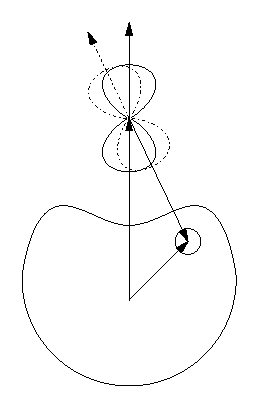
\includegraphics{DIM-axis}}%
    \gplfronttext
  \end{picture}%
\endgroup
}
\caption{Set of axes involved in our description\label{fig:DIM-axis}}
\end{minipage}
\end{figure}

We now define $U^{nl}_{ij\alpha\beta}$ which is simply the pair-interaction Hamiltonian expressed in the common basis
\begin{align}
U^{nl/\DIM}_{ij\alpha\beta}(\vb{r}_m) &= \bra{i,\alpha} \mathcal{R}_m^{-1} H^{nl/\DIM}_\KHE(\vb{r}_m) \, \mathcal{R}_m \ket{j,\beta}
\end{align}
The matrix elements of the total electrostatic Hamiltonian can then be expressed in the discrete case (helium atoms) or in the continuum case (helium density) as
\begin{align}
E^{nl/\DIM}_{ij\alpha\beta}(\{\vb{r}_m\}) &= \sum_{m=1}^{m=N} U^{nl/\DIM}_{ij\alpha\beta}(\vb{r}_m) \\
E^{nl/\DIM}_{ij\alpha\beta} (\vb{r}_\K) &= \int \dd{\vb{r}} \rho(\vb{r} + \vb{r}_\K) \, \bra{i,\alpha} \mathcal{R}^{-1}(\vb{r}) H^{nl/\DIM}_\KHE(\vb{r}) \, \mathcal{R}(\vb{r}) \ket{j,\beta} \equiv \int \dd{\vb{r}} \rho(\vb{r} + \vb{r}_\K) \, U_{ij\alpha\beta}^{nl/\DIM}(\vb{r}) \label{eq:DIM-defE}
\end{align}

\subsubsection{Spherically symmetric ($ns$) state}

Let us first consider the two ($ns$) states: ($4s$) and ($5s$). They are particularly easy to treat because the spin-orbit coupling can be omitted since $L=0$ (see \citeq{eq:DIM-HSO}). We are left with the electrostatic contribution, which is also easy to express because $s$-states are  spherically symmetric, hence invariant under rotation about they symmetry center
\begin{align*}
U^{ns/\DIM}_{ij\alpha\beta}(\vb{r}_m) &= \bra{i,\alpha} \mathcal{R}_m^{-1} H^{nl/\DIM}_\KHE(\vb{r}_m) \, \mathcal{R}_m \ket{j,\beta} \\
&= V^{ns}(\vb{r}_m) \, \bra{i,\alpha} \mathcal{R}_m^{-1} \ket{ns_m}\bra{ns_m} \, \mathcal{R}_m \ket{j,\beta} \\
&= V^{ns}(\vb{r}_m) \, \braket{i,\alpha}{ns_m}\braket{ns_m}{j,\beta} \\
&= V^{ns}(\vb{r}_m) \, \delta_{ij} \delta_{\alpha\beta}\num\\
E^{ns/\DIM}_{ij\alpha\beta} (\vb{r}_\K) &= \int \dd{\vb{r}} \rho(\vb{r} + \vb{r}_\K) \, V^{ns}(\vb{r}) \, \delta_{ij} \delta_{\alpha\beta}\num
\end{align*}

The matrix elements are clearly diagonal in the common basis $\{\ket{ns,\pm}\}$, moreover they do not depend on spin state. 
In order to represent the interaction (\citfig{fig:DIM-5s-pot}) we can plot $V^{ns}$ which is the KHe pair interaction  (in the unrotated frame) and $E^{nl}_{ss\alpha\alpha}$ which is the averaged potential: it represents the potential felt by a diabatically displaced K, this actually gives a snapshot of the system at $t=0$. 
We will discuss in \citsec{sec:4S-dia} the meaning of adiabatic \textit{vs} diabatic hypothesis and their reliability. 
\begin{figure}[h!] 
\centering
    % GNUPLOT: LaTeX picture with Postscript
\begingroup
  \makeatletter
  \providecommand\color[2][]{%
    \GenericError{(gnuplot) \space\space\space\@spaces}{%
      Package color not loaded in conjunction with
      terminal option `colourtext'%
    }{See the gnuplot documentation for explanation.%
    }{Either use 'blacktext' in gnuplot or load the package
      color.sty in LaTeX.}%
    \renewcommand\color[2][]{}%
  }%
  \providecommand\includegraphics[2][]{%
    \GenericError{(gnuplot) \space\space\space\@spaces}{%
      Package graphicx or graphics not loaded%
    }{See the gnuplot documentation for explanation.%
    }{The gnuplot epslatex terminal needs graphicx.sty or graphics.sty.}%
    \renewcommand\includegraphics[2][]{}%
  }%
  \providecommand\rotatebox[2]{#2}%
  \@ifundefined{ifGPcolor}{%
    \newif\ifGPcolor
    \GPcolortrue
  }{}%
  \@ifundefined{ifGPblacktext}{%
    \newif\ifGPblacktext
    \GPblacktextfalse
  }{}%
  % define a \g@addto@macro without @ in the name:
  \let\gplgaddtomacro\g@addto@macro
  % define empty templates for all commands taking text:
  \gdef\gplbacktext{}%
  \gdef\gplfronttext{}%
  \makeatother
  \ifGPblacktext
    % no textcolor at all
    \def\colorrgb#1{}%
    \def\colorgray#1{}%
  \else
    % gray or color?
    \ifGPcolor
      \def\colorrgb#1{\color[rgb]{#1}}%
      \def\colorgray#1{\color[gray]{#1}}%
      \expandafter\def\csname LTw\endcsname{\color{white}}%
      \expandafter\def\csname LTb\endcsname{\color{black}}%
      \expandafter\def\csname LTa\endcsname{\color{black}}%
      \expandafter\def\csname LT0\endcsname{\color[rgb]{1,0,0}}%
      \expandafter\def\csname LT1\endcsname{\color[rgb]{0,1,0}}%
      \expandafter\def\csname LT2\endcsname{\color[rgb]{0,0,1}}%
      \expandafter\def\csname LT3\endcsname{\color[rgb]{1,0,1}}%
      \expandafter\def\csname LT4\endcsname{\color[rgb]{0,1,1}}%
      \expandafter\def\csname LT5\endcsname{\color[rgb]{1,1,0}}%
      \expandafter\def\csname LT6\endcsname{\color[rgb]{0,0,0}}%
      \expandafter\def\csname LT7\endcsname{\color[rgb]{1,0.3,0}}%
      \expandafter\def\csname LT8\endcsname{\color[rgb]{0.5,0.5,0.5}}%
    \else
      % gray
      \def\colorrgb#1{\color{black}}%
      \def\colorgray#1{\color[gray]{#1}}%
      \expandafter\def\csname LTw\endcsname{\color{white}}%
      \expandafter\def\csname LTb\endcsname{\color{black}}%
      \expandafter\def\csname LTa\endcsname{\color{black}}%
      \expandafter\def\csname LT0\endcsname{\color{black}}%
      \expandafter\def\csname LT1\endcsname{\color{black}}%
      \expandafter\def\csname LT2\endcsname{\color{black}}%
      \expandafter\def\csname LT3\endcsname{\color{black}}%
      \expandafter\def\csname LT4\endcsname{\color{black}}%
      \expandafter\def\csname LT5\endcsname{\color{black}}%
      \expandafter\def\csname LT6\endcsname{\color{black}}%
      \expandafter\def\csname LT7\endcsname{\color{black}}%
      \expandafter\def\csname LT8\endcsname{\color{black}}%
    \fi
  \fi
    \setlength{\unitlength}{0.0500bp}%
    \ifx\gptboxheight\undefined%
      \newlength{\gptboxheight}%
      \newlength{\gptboxwidth}%
      \newsavebox{\gptboxtext}%
    \fi%
    \setlength{\fboxrule}{0.5pt}%
    \setlength{\fboxsep}{1pt}%
\begin{picture}(9360.00,5760.00)%
    \gplgaddtomacro\gplbacktext{%
      \csname LTb\endcsname%
      \put(991,2230){\makebox(0,0)[r]{\strut{}$30000$}}%
      \put(991,2588){\makebox(0,0)[r]{\strut{}$30150$}}%
      \put(991,2947){\makebox(0,0)[r]{\strut{}$30300$}}%
      \put(991,3305){\makebox(0,0)[r]{\strut{}$30450$}}%
      \put(991,3664){\makebox(0,0)[r]{\strut{}$30600$}}%
      \put(991,4022){\makebox(0,0)[r]{\strut{}$30750$}}%
      \put(991,4381){\makebox(0,0)[r]{\strut{}$30900$}}%
      \put(991,4739){\makebox(0,0)[r]{\strut{}$31050$}}%
      \put(991,5098){\makebox(0,0)[r]{\strut{}$31200$}}%
      \put(991,5456){\makebox(0,0)[r]{\strut{}$31350$}}%
      \put(199,3167){\rotatebox{90}{\makebox(0,0){\strut{}Energy (K)}}}%
      \put(5194,149){\makebox(0,0){\strut{}Distance from equilibrium position (\AA)}}%
    }%
    \gplgaddtomacro\gplfronttext{%
      \csname LTb\endcsname%
      \put(8128,5293){\makebox(0,0)[r]{\strut{}$5s$}}%
      \csname LTb\endcsname%
      \put(8128,5073){\makebox(0,0)[r]{\strut{}4s}}%
    }%
    \gplgaddtomacro\gplbacktext{%
      \csname LTb\endcsname%
      \put(991,776){\makebox(0,0)[r]{\strut{}$-15$}}%
      \put(991,1015){\makebox(0,0)[r]{\strut{}$-10$}}%
      \put(991,1254){\makebox(0,0)[r]{\strut{}$-5$}}%
      \put(991,1493){\makebox(0,0)[r]{\strut{}$0$}}%
      \put(1344,413){\makebox(0,0){\strut{}$-6$}}%
      \put(1786,413){\makebox(0,0){\strut{}$-4$}}%
      \put(2228,413){\makebox(0,0){\strut{}$-2$}}%
      \put(2670,413){\makebox(0,0){\strut{}$0$}}%
      \put(3112,413){\makebox(0,0){\strut{}$2$}}%
      \put(3553,413){\makebox(0,0){\strut{}$4$}}%
      \put(3995,413){\makebox(0,0){\strut{}$6$}}%
      \put(4437,413){\makebox(0,0){\strut{}$8$}}%
      \put(4879,413){\makebox(0,0){\strut{}$10$}}%
    }%
    \gplgaddtomacro\gplfronttext{%
    }%
    \gplgaddtomacro\gplbacktext{%
    }%
    \gplgaddtomacro\gplfronttext{%
    }%
    \gplgaddtomacro\gplbacktext{%
      \csname LTb\endcsname%
      \put(5509,413){\makebox(0,0){\strut{}$-2$}}%
      \put(5951,413){\makebox(0,0){\strut{}$0$}}%
      \put(6393,413){\makebox(0,0){\strut{}$2$}}%
      \put(6835,413){\makebox(0,0){\strut{}$4$}}%
      \put(7277,413){\makebox(0,0){\strut{}$6$}}%
      \put(7718,413){\makebox(0,0){\strut{}$8$}}%
      \put(8160,413){\makebox(0,0){\strut{}$10$}}%
      \put(8602,413){\makebox(0,0){\strut{}$12$}}%
      \put(9044,413){\makebox(0,0){\strut{}$14$}}%
    }%
    \gplgaddtomacro\gplfronttext{%
    }%
    \gplbacktext
    \put(0,0){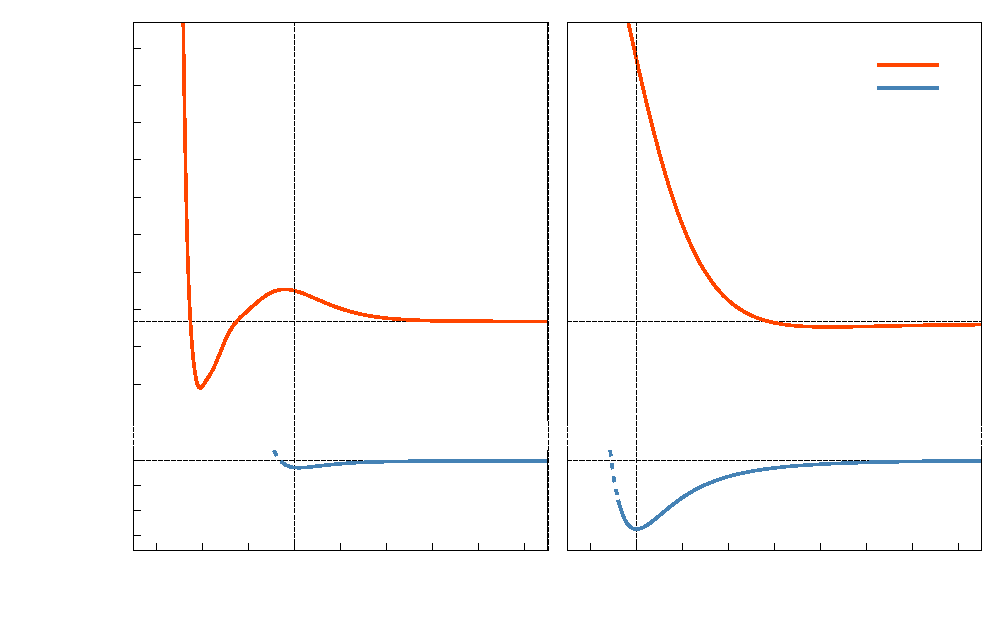
\includegraphics{DIM-5s-pot}}%
    \gplfronttext
  \end{picture}%
\endgroup

    \vspace{-0.5\baselineskip}
    \caption{Pair potential (left) and averaged interaction over the droplet (right). Equilibrium distances: $r=7.0$ \AA{} for KHe and $r=26.3$ \AA{} (between centers of mass) for KHe$_{1000}$}
    \label{fig:DIM-5s-pot}
\end{figure}
 \vspace{-1\baselineskip}
\subsubsection{An in-depth description with the ($4p$) state}
\label{sec:DIM-4p}

The ($4p$) state is more involved since it corresponds to $L=1$: on the one hand it no longer has spherical symmetry but cylindrical symmetry, and on the other hand spin-orbit coupling has to be taken into account. 
Let us first focus on the electrostatic interaction. 
\begin{align*}
U^{4p/\DIM}_{ij\alpha\beta}(\vb{r}_m) &= \bra{i,\alpha} \mathcal{R}_m^{-1} H^{4p/\DIM}_\KHE(\vb{r}_m) \, \mathcal{R}_m \ket{j,\beta} \\
&= \bra{i,\alpha} \mathcal{R}_m^{-1} \left(V^{4p}_\Pi(\vb{r}_n) \, \mathbb{I}_3 + [V^{4p}_\Sigma(\vb{r}_n) -V^{4p}_\Pi(\vb{r}_n) ]  \ket{p_{z_n}}\bra{p_{z_n}} \right) \, \mathcal{R}_m \ket{j,\beta} \\
&= \bra{i,\alpha} \left(V^{4p}_\Pi(\vb{r}_n) \, \mathbb{I}_3 + [V^{4p}_\Sigma(\vb{r}_n) -V^{4p}_\Pi(\vb{r}_n) ]   \{ \mathcal{R}_m^{-1}\ket{p_{z_n}}\bra{p_{z_n}}\mathcal{R}_m\} \right) \,  \ket{j,\beta} \num\\
&= \left(  V^{4p}_\Pi(\vb{r}_n) \, \delta_{ij}   + [V^{4p}_\Sigma(\vb{r}_n) -V^{4p}_\Pi(\vb{r}_n) ] \bra{i} \mathcal{R}_m^{-1}\ket{p_{z_n}}\bra{p_{z_n}}\mathcal{R}_m\ket{j} \right) \, \delta_{\alpha\beta}\num
\end{align*}

Expressing the interaction in a set of real orbitals makes the expression of the rotation easier because they transform as $\mathbb{R}^3$ vectors
\begin{align}
\bra{i} \mathcal{R}_m^{-1} \ket{p_{z_m}} \bra{p_{z_m}} \mathcal{R}_m \ket{j} = \frac{x^i_m \, x^j_m}{\|\vb{r}_m\|^2}
\end{align}

We can then write the electrostatic matrix elements
\begin{align}
U^{4p/\DIM}_{ij\alpha\beta}(\vb{r}_m) &= \left( V_\Pi(\vb{r}_m) \, \delta_{ij} + [V_\Sigma(\vb{r}_m) -V_\Pi(\vb{r}_m) ] \, \frac{x^i_m \, x^j_m}{\|\vb{r}_m\|^2} \right) \, \delta_{\alpha\beta} \label{eq:DIM-udef} \\
E^{4p/\DIM}_{ij\alpha\beta}(\vb{r}_\K) &= \int \dd{\vb{r}} \rho(\vb{r} + \vb{r}_\K) \, \left( V_\Pi(\vb{r}) \, \delta_{ij} + [V_\Sigma(\vb{r}) -V_\Pi(\vb{r}) ] \, \frac{x^i \, x^j}{\|\vb{r}\|^2} \right) \, \delta_{\alpha\beta}
\end{align}

Diagonalizing the electrostatic Hamiltonian within cylindrical symmetry\footnote{The ground state helium droplet being spherical, the ground state for K-He$_N$ has cylindrical symmetry, and this symmetry is conserved upon excitation.} gives a set of eigenvalues $\{ \varepsilon\}$

\begin{align*}
\varepsilon_i(\vb{r}_\K) = E^{4p/\DIM}_{ii\alpha\alpha}(\vb{r}_\K) = 2\pi \iint & r^2 \sin\theta \dd{\theta} \dd{r} \, \rho\left(\sqrt{|r^2 + r_\K^2 + 2r r_\K \cos\theta|}\right) \\
& \left( V_\Pi(r) + [V_\Sigma(r) -V_\Pi(r) ] \, \left[\frac{1}{2}(\delta_{ip_x}+\delta_{ip_y}) \sin^2\theta + \delta_{ip_z} \cos^2 \theta \right] \right) \num
\end{align*}
Because of the overall cylindrical symmetry we see that the Hamiltonian is diagonal in the common basis.
In particular the associated eigenvectors are the real $4p$-orbitals $\{ \ket{4p_{x},\pm},\ket{4p_{y},\pm},\ket{4p_{z}},\pm\}$\footnote{Note that these states are actually doubly degenerate because of spin degeneracy} and $\Lambda$ is a good quantum number. \\

We now turn to the spin-orbit interaction in the same basis set, which is known as the \textit{uncoupled} basis set: $\{\ket{p_x,+}, \ket{p_x,-}, \ket{p_y,+}, \ket{p_y,-}, \ket{p_z,+}, \ket{p_z,-} \}$. 
The matrix elements of the spin-orbit Hamiltonian are more easily expressed in the basis set of (complex) orbitals with a well defined value of $\Lambda$, and then transformed back to the real (cartesian) orbitals. We end up with

\begin{align}
H^{4p/\SO} &= A_\LS \, \vb{L}\cdot\vb{S} = A_\LS \, (L_+S_- + L_-S_+ + L_z S_z)	 
= \frac{A_\LS}{2} \mqty(	0 &  0 & -i &  0 &  0 &  1 \\
 			 				 	0 &  0 &  0 &  i & -1 &  0 \\
 			 				 	i &  0 &  0 &  0 &  0 & -i \\
 			 					0 & -i &  0 &  0 & -i &  0 \\
 								0 & -1 &  0 &  i &  0 &  0 \\
 			 					1 &  0 &  i &  0 &  0 &  0)				
\end{align}

The matrix elements of the full Hamiltonian are then
\begin{align}
U^{4p}_{ij\alpha\beta}(\vb{r}_m) &= U^{4p/\DIM}_{ij\alpha\beta}(\vb{r}_m) + U^{4p/\SO}_{ij\alpha\beta}\\
E^{4p}_{ij\alpha\beta}(\vb{r}_\K) &= \int \dd{\vb{r}} \rho(\vb{r} + \vb{r}_\K) \, \left( V_\Pi(\vb{r}) \, \delta_{ij} + [V_\Sigma(\vb{r}) -V_\Pi(\vb{r}) ] \, \frac{x^i \, x^j}{\|\vb{r}\|^2} \right) \, \delta_{\alpha\beta} + U^{4p/\SO}_{ij\alpha\beta} \\
\end{align}

Its diagonalization gives the set of eigenvalues $\{\xi\}$
\begin{align*}
\xi_1(\vb{r}_\K) &= \frac{1}{2} (\varepsilon_1 + \varepsilon_3) + \frac{1}{4}\left(-A_\LS+\sqrt{9 A_\LS^2-4 A_\LS(\varepsilon_1-\varepsilon_3) + 4(\varepsilon_1-\varepsilon_3)^2}\right) \\		
\xi_2(\vb{r}_\K) &= \varepsilon_1 + \frac{A_\LS}{2} \label{eq:DIM-SO-nrj} \num \\
\xi_3(\vb{r}_\K) &= \frac{1}{2} (\varepsilon_1 + \varepsilon_3) + \frac{1}{4}\left(-A_\LS-\sqrt{9 A_\LS^2-4 A_\LS(\varepsilon_1-\varepsilon_3) + 4(\varepsilon_1-\varepsilon_3)^2}\right)
\end{align*}

\begin{table}[!h]
\centering
\begin{tabular}{|c|c|c|c|}
\hline
 & $\xi_1$ & $\xi_2$ & $\xi_3$  \\
\hline
Value when $\varepsilon_i \ll A_\LS$ & $+\frac{A_\LS}{2}$ & $+\frac{A_\LS}{2}$ & $-A_\LS$\\  
\hline
Associated $J$ value & $3/2$ & $3/2$ & $1/2$\\  
\hline
Value when $\varepsilon_i \gg A_\LS$ & $\varepsilon_3$ & $\varepsilon_1$ & $\varepsilon_1$ \\
\hline
Associated $|\Lambda|$ value & $0$ & $1$  & $1$  \\
\hline
Associated $|\Omega|$ value & $1/2$ & $3/2$ & $1/2$ \\
\hline
Label & $\Sigma_{1/2}$ & $\Pi_{3/2}$ & $ \Pi_{1/2}$ \\
\hline
\end{tabular}
\caption{Determination of true good quantum number $\Omega$ and approximate ones $\Lambda$ and $J$}
\label{table:DIM-labels}
\end{table}

\begin{figure}[h!]
\centering
    % GNUPLOT: LaTeX picture with Postscript
\begingroup
  \makeatletter
  \providecommand\color[2][]{%
    \GenericError{(gnuplot) \space\space\space\@spaces}{%
      Package color not loaded in conjunction with
      terminal option `colourtext'%
    }{See the gnuplot documentation for explanation.%
    }{Either use 'blacktext' in gnuplot or load the package
      color.sty in LaTeX.}%
    \renewcommand\color[2][]{}%
  }%
  \providecommand\includegraphics[2][]{%
    \GenericError{(gnuplot) \space\space\space\@spaces}{%
      Package graphicx or graphics not loaded%
    }{See the gnuplot documentation for explanation.%
    }{The gnuplot epslatex terminal needs graphicx.sty or graphics.sty.}%
    \renewcommand\includegraphics[2][]{}%
  }%
  \providecommand\rotatebox[2]{#2}%
  \@ifundefined{ifGPcolor}{%
    \newif\ifGPcolor
    \GPcolortrue
  }{}%
  \@ifundefined{ifGPblacktext}{%
    \newif\ifGPblacktext
    \GPblacktextfalse
  }{}%
  % define a \g@addto@macro without @ in the name:
  \let\gplgaddtomacro\g@addto@macro
  % define empty templates for all commands taking text:
  \gdef\gplbacktext{}%
  \gdef\gplfronttext{}%
  \makeatother
  \ifGPblacktext
    % no textcolor at all
    \def\colorrgb#1{}%
    \def\colorgray#1{}%
  \else
    % gray or color?
    \ifGPcolor
      \def\colorrgb#1{\color[rgb]{#1}}%
      \def\colorgray#1{\color[gray]{#1}}%
      \expandafter\def\csname LTw\endcsname{\color{white}}%
      \expandafter\def\csname LTb\endcsname{\color{black}}%
      \expandafter\def\csname LTa\endcsname{\color{black}}%
      \expandafter\def\csname LT0\endcsname{\color[rgb]{1,0,0}}%
      \expandafter\def\csname LT1\endcsname{\color[rgb]{0,1,0}}%
      \expandafter\def\csname LT2\endcsname{\color[rgb]{0,0,1}}%
      \expandafter\def\csname LT3\endcsname{\color[rgb]{1,0,1}}%
      \expandafter\def\csname LT4\endcsname{\color[rgb]{0,1,1}}%
      \expandafter\def\csname LT5\endcsname{\color[rgb]{1,1,0}}%
      \expandafter\def\csname LT6\endcsname{\color[rgb]{0,0,0}}%
      \expandafter\def\csname LT7\endcsname{\color[rgb]{1,0.3,0}}%
      \expandafter\def\csname LT8\endcsname{\color[rgb]{0.5,0.5,0.5}}%
    \else
      % gray
      \def\colorrgb#1{\color{black}}%
      \def\colorgray#1{\color[gray]{#1}}%
      \expandafter\def\csname LTw\endcsname{\color{white}}%
      \expandafter\def\csname LTb\endcsname{\color{black}}%
      \expandafter\def\csname LTa\endcsname{\color{black}}%
      \expandafter\def\csname LT0\endcsname{\color{black}}%
      \expandafter\def\csname LT1\endcsname{\color{black}}%
      \expandafter\def\csname LT2\endcsname{\color{black}}%
      \expandafter\def\csname LT3\endcsname{\color{black}}%
      \expandafter\def\csname LT4\endcsname{\color{black}}%
      \expandafter\def\csname LT5\endcsname{\color{black}}%
      \expandafter\def\csname LT6\endcsname{\color{black}}%
      \expandafter\def\csname LT7\endcsname{\color{black}}%
      \expandafter\def\csname LT8\endcsname{\color{black}}%
    \fi
  \fi
    \setlength{\unitlength}{0.0500bp}%
    \ifx\gptboxheight\undefined%
      \newlength{\gptboxheight}%
      \newlength{\gptboxwidth}%
      \newsavebox{\gptboxtext}%
    \fi%
    \setlength{\fboxrule}{0.5pt}%
    \setlength{\fboxsep}{1pt}%
\begin{picture}(9360.00,5760.00)%
    \gplgaddtomacro\gplbacktext{%
      \csname LTb\endcsname%
      \put(991,1877){\makebox(0,0)[r]{\strut{}$18350$}}%
      \put(991,2259){\makebox(0,0)[r]{\strut{}$18400$}}%
      \put(991,2642){\makebox(0,0)[r]{\strut{}$18450$}}%
      \put(991,3024){\makebox(0,0)[r]{\strut{}$18500$}}%
      \put(991,3407){\makebox(0,0)[r]{\strut{}$18550$}}%
      \put(991,3789){\makebox(0,0)[r]{\strut{}$18600$}}%
      \put(991,4171){\makebox(0,0)[r]{\strut{}$18650$}}%
      \put(991,4554){\makebox(0,0)[r]{\strut{}$18700$}}%
      \put(991,4936){\makebox(0,0)[r]{\strut{}$18750$}}%
      \put(991,5319){\makebox(0,0)[r]{\strut{}$18800$}}%
      \put(991,5701){\makebox(0,0)[r]{\strut{}$18850$}}%
      \put(199,3167){\rotatebox{90}{\makebox(0,0){\strut{}Energy (K)}}}%
      \put(5194,149){\makebox(0,0){\strut{}Distance from equilibrium position (\AA)}}%
    }%
    \gplgaddtomacro\gplfronttext{%
      \csname LTb\endcsname%
      \put(8260,3210){\makebox(0,0)[r]{\strut{}$\Pi_{1/2}$}}%
      \csname LTb\endcsname%
      \put(8260,2990){\makebox(0,0)[r]{\strut{}$\Pi_{3/2}$}}%
      \csname LTb\endcsname%
      \put(8260,2770){\makebox(0,0)[r]{\strut{}$\Sigma_{1/2}$}}%
      \csname LTb\endcsname%
      \put(8260,2550){\makebox(0,0)[r]{\strut{}4s}}%
    }%
    \gplgaddtomacro\gplbacktext{%
      \csname LTb\endcsname%
      \put(991,776){\makebox(0,0)[r]{\strut{}$-15$}}%
      \put(991,1015){\makebox(0,0)[r]{\strut{}$-10$}}%
      \put(991,1254){\makebox(0,0)[r]{\strut{}$-5$}}%
      \put(991,1493){\makebox(0,0)[r]{\strut{}$0$}}%
      \put(1123,413){\makebox(0,0){\strut{}$-6$}}%
      \put(1735,413){\makebox(0,0){\strut{}$-4$}}%
      \put(2347,413){\makebox(0,0){\strut{}$-2$}}%
      \put(2959,413){\makebox(0,0){\strut{}$0$}}%
      \put(3570,413){\makebox(0,0){\strut{}$2$}}%
      \put(4182,413){\makebox(0,0){\strut{}$4$}}%
      \put(4794,413){\makebox(0,0){\strut{}$6$}}%
    }%
    \gplgaddtomacro\gplfronttext{%
    }%
    \gplgaddtomacro\gplbacktext{%
    }%
    \gplgaddtomacro\gplfronttext{%
    }%
    \gplgaddtomacro\gplbacktext{%
      \csname LTb\endcsname%
      \put(5441,413){\makebox(0,0){\strut{}$-2$}}%
      \put(6053,413){\makebox(0,0){\strut{}$0$}}%
      \put(6665,413){\makebox(0,0){\strut{}$2$}}%
      \put(7277,413){\makebox(0,0){\strut{}$4$}}%
      \put(7888,413){\makebox(0,0){\strut{}$6$}}%
      \put(8500,413){\makebox(0,0){\strut{}$8$}}%
      \put(9112,413){\makebox(0,0){\strut{}$10$}}%
    }%
    \gplgaddtomacro\gplfronttext{%
    }%
    \gplbacktext
    \put(0,0){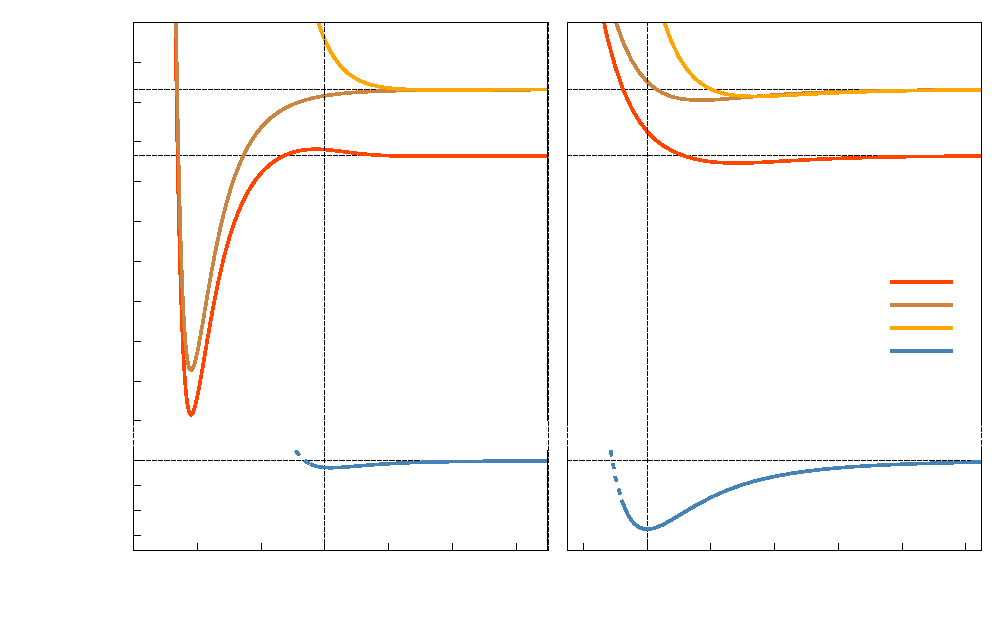
\includegraphics{DIM-p-pot}}%
    \gplfronttext
  \end{picture}%
\endgroup

    \vspace{-0.5\baselineskip}
    \caption{Pair potential (left) and averaged interaction over the droplet (right)}
    \label{fig:DIM-4p-pot}
\end{figure}

We present in \cittab{table:DIM-labels} the reasoning used to determine the true good quantum number $\Omega$ and the approximate ones: $\Lambda$ and $J$. 
We use the following label $\Lambda_\Omega$ for energy states. % (Hund's case (a) for coupling of angular momenta).
$J$ does not appear because in the excitation region the $\Sigma-\Pi$ splitting between electrostatic eigenvalues is larger that the atomic spin-orbit splitting, such that $\Lambda$ gives a better representation of the reality.\\

In the same way than for the ($5s$) state (\citfig{fig:DIM-5s-pot}), we plot both the pair interaction and the averaged potential in \citfig{fig:DIM-4p-pot}. Keep in mind that pair potential refers to the unrotated basis, for instance in a global $\Pi_{1/2}$ state, there are only the helium in the internuclear axis that interact with $\Pi_{1/2}$ potential. Note also that the averaged potential corresponds to one of the $\xi$ value labeled according to the previous discussion.

\subsection{Writing energy contribution to doped helium droplet}

In order to describe the electronic degree of freedom, we introduce the electronic wave function $\ket{\lambda}$
\begin{align}
\ket{\lambda} = \sum_{\underset{i\in \{nl \, \text{orbitals}\}}{\alpha=\{+,-\}}} \lambda_{i\alpha} \ket{i,\alpha}
\label{eq:DIM-lambda-state}
\end{align}

Let us consider the interaction Hamiltonian for $H^{nl}_\KHEN(\vb{r}_\K)$ (\citeq{eq:DIM-hamtot}), we will write the corresponding interaction in the continuum formalism. 
We first describe the total energy for a point-like interaction, \textit{id est} a classical particle
\begin{align}
E[\rho] \rightarrow E[\rho, \vb{r}_\K,\lambda] &= E[\rho]  + \bra{\Psi,\lambda}H^{nl}_\KHEN(\vb{r}_\K)\ket{\Psi,\lambda} \label{eq:DIM-C-nrj-correction}
\end{align}
The interaction part is given by
\begin{align}
\bra{\Psi,\lambda}H^{nl}_\KHEN\ket{\Psi,\lambda} &= \int \dd{\vb{r}} \, \rho(\vb{r}+\vb{r}_\K) \bra{\lambda} \mathcal{R}^{-1}(\vb{r}) H^{nl/\DIM}_\KHE(\vb{r}) \, \mathcal{R}(\vb{r})\ket{\lambda} + \bra{\lambda}H^{nl/\SO} \ket{\lambda}\\
&\equiv \int \dd{\vb{r}} \, \rho(\vb{r}) \, V_\KHE^{nl\lambda}(\vb{r}-\vb{r}_\K) +  \bra{\lambda}H^{nl/\SO} \ket{\lambda}
\end{align}
where the time evolution of the \emph{effective} potential is given by that of the electronic wave packet $\ket{\lambda}$, using notation of \citeq{eq:DIM-udef}
\begin{align}
V_\KHE^{nl\lambda}(\vb{r}) &= \bra{\lambda} \mathcal{R}^{-1}(\vb{r}) H^{nl/\DIM}_\KHE(\vb{r}) \, \mathcal{R}(\vb{r})\ket{\lambda} =  \sum_{ij\alpha\beta} \lambda_{i\alpha}^* \, U^{nl/\DIM}_{ij\alpha\beta}(\vb{r}) \, \lambda_{j\beta}
\end{align}

For a quantum particle described by a wave function $\phi$, \citeq{eq:DIM-C-nrj-correction} becomes
\begin{align}
E[\rho] \rightarrow E[\rho, \phi,\lambda] &= E[\rho]  + \bra{\Psi,\lambda, \phi}H^{nl}_\KHEN(\vb{r}_\K)\ket{\Psi,\lambda, \phi}
\end{align}

In the classical case, variation of the total energy with respect to the effective helium wave function (order parameter) $\Psi$ gives the \textsc{Euler-Lagrange} equations.

\begin{align}
&E[\rho,\vb{r}_\K,\lambda] = E[\rho] + \int \dd{\vb{r}} \, \rho(\vb{r}) V^{nl\lambda}_\KHE(\vb{r}-\vb{r}_\K) + \bra{\lambda}H^{nl/\SO}\ket{\lambda} \\
&\Rightarrow \left( -\frac{\hbar^2}{2m_\K} \grad{}^2 + \frac{\delta \mathcal{E}_c}{\delta \rho} + V^{nl\lambda}_\KHE(\vb{r}-\vb{r}_\K)\right)\Psi(\vb{r})=\mu \Psi(\vb{r})
\end{align}

In the quantum case one adds variation with respect to the alkali wave function, which yields two coupled equations
\begin{align*}
&E[\rho,\phi,\lambda] = E[\rho] + \iint \dd{\vb{r}}\dd{\vb{r}_\K} \, \rho(\vb{r}) V^{nl\lambda}_\KHE(\vb{r}-\vb{r}_\K) |\phi(\vb{r}_\K)|^2 \\
& \qquad \qquad \qquad \qquad \qquad \qquad \qquad + \frac{\hbar^2}{2m_\K} \int \dd{\vb{r}_\K} |\grad{}_{\vb{r}_\K}\phi(\vb{r}_\K)|^2 + \bra{\lambda}H^{nl/\SO}\ket{\lambda} \num \\
&\Rightarrow \left\{
\begin{array}{l}
  \left( -\frac{\hbar^2}{2m_\HE} \grad{}_{\vb{r}}^2 + \frac{\delta \mathcal{E}_c}{\delta \rho} + \int \dd{\vb{r}_\K} \,V^{nl\lambda}_\KHE(\vb{r}-\vb{r}_\K)|\phi(\vb{r}_\K)|^2 \right)\Psi(\vb{r})=\mu \Psi(\vb{r})\\
\left( -\frac{\hbar^2}{2m_\K} \grad{}_{\vb{r}_\K}^2 + \int \dd{\vb{r}} \,V^{nl\lambda}_\KHE(\vb{r}-\vb{r}_\K)\rho(\vb{r}) \right)\phi(\vb{r}_\K)=\varepsilon \phi(\vb{r}_\K)
\end{array}
\right. \num 
\end{align*}

We see that thanks to the introduction of the \textit{order parameter} these equations look like \textsc{Schrodinger} equations.
Technical details on how to solve these equations are given in the \citanx{sec:ANX-itp}.

\section{TDDFT}

The purpose of this work is to study the dynamic evolution of our system under absorption of a photon. 
Hence in this section we describe the method used for the dynamics.
It is based on the \textsc{Runge-Gross} theorem \cite{Run1984} which extends the DFT formalism to time dependent studies (TD-DFT).

\subsection{Excitation process}

We assume that the exciting laser pulse is very short, so that the nuclei do not have time to move (``vertical transition'').
This amounts to considering that the initial conditions for the dynamics are the ground equilibrium helium density and alkali position for the nuclei, and that the electronic state is suddenly switched to the excited state $(4p)$ or $(5s)$. In other words, we start a dynamic study with a new interaction Hamiltonian but with the ground state density, this is equivalent to the \textsc{Franck-Condon} approximation with a constant transition dipole moment.

\subsection{Classical dynamics}

TD-DFT is based on the variation of the action $\mathcal{A}$ (instead of energy in DFT) with respect to all its parameters
\begin{align}
\mathcal{A}[\Psi,\vb{r}_\K,\lambda] = \int \dd{t} \left( E[\Psi,\vb{r}_\K,\lambda] - i\hbar \int \dd{\vb{r}} \Psi^*(\vb{r},t) \pdv{t} \Psi(\vb{r},t) - i\hbar \bra{\lambda} \pdv{t} \ket{\lambda} - \frac{1}{2} m_\K \vb{\dot{r}}_\K^2\right)
\end{align}

This procedure yields to a set of three coupled equations that govern the dynamics (computational details are described in the \citanx{sec:ANX-rtp}).
\begin{align}
i\hbar \pdv{t} \Psi(\vb{r},t)  &= \left(-\frac{\hbar^2}{2m_\HE} \grad{}^2_{\vb{r}} + \frac{\delta \mathcal{E}_c}{\delta \rho(\vb{r})}  + V_\KHE^{nl\lambda} (\vb{r}-\vb{r}_\K)\right) \Psi(\vb{r},t) \\
i\hbar \pdv{t} \ket{\lambda} &= H_\KHEN^{nl}(\vb{r}_\K) \ket{\lambda} \\
m_\K \vb{\ddot{r}}_\K &= -\grad{}_{\vb{r}_\K} \left(\int \dd{\vb{r}} \rho(\vb{r}) V_\KHE^{nl\lambda}(\vb{r}-\vb{r}_\K) \right) = - \left(\int \dd{\vb{r}}  V_\KHE^{nl\lambda}(\vb{r}-\vb{r}_\K)\grad{}_{\vb{r}}\rho(\vb{r}) \right)
\end{align}

\subsection{Test particles and quantum dynamics in an isotrotropic state}

We could use the same procedure as for treating K quantum mechanically in the statics. However, the potassium atom can acquire a rather high kinetic energy when dissociating, and this is impossible to describe with the same grid as that of the helium density.
Instead we used a test particles method based on Bohmian dynamics, as proposed by Hernando \textit{et al.} \cite{Her2012} for Li and Na photodissociation from a helium droplet. \\

The starting point is to write the impurity complex wave function in the exponential with modulus $\psi(\vb{r},t)$ and phase $\mathcal{S}(\vb{r},t)$, $\psi$ and $\mathcal{S}$ being two real and positive functions
\begin{align}
\phi(\vb{r},t) &= \psi(\vb{r},t)\, \e^{i\mathcal{S}(\vb{r},t)/\hbar} 
\end{align}

We set $\vb{v}= \frac{1}{m_\K} \grad{} \mathcal{S}$, then the current density $\vb{j} = \frac{\hbar}{2m_\K} \left(\phi^* \grad{} \phi - \phi \grad \phi^* \right)$ becomes $\vb{j} = \psi^2 \, \vb{v}$. Finally the \textsc{Schrödinger} equation gives a coupled system of equations
\begin{align}
\pdv{\psi^2(\vb{r},t)}{t} &= - \grad{} \cdot \vb{j}(\vb{r},t) \label{eq:TDDFT-cont} \\
- \pdv{\mathcal{S}(\vb{r},t)}{t} &= \frac{1}{2} m_\K \vb{v}^2(\vb{r},t) + \mathcal{Q}(\vb{r},t) + V(\vb{r}) \with \mathcal{Q} = -\frac{\hbar^2}{2m_\K} \frac{\grad{}^2 \psi}{\psi} \label{eq:TDDFT-HJ} 
\end{align}

Then, we consider a set of $M$ particles with trajectories $\{\vb{R_j}(t)\}$ with $\vb{R}_i(t)=\vb{R}(\vb{r}_i,t)$ and $\vb{R}_i(0)=\vb{r}_i$ such that
\begin{align}
\psi(\vb{r},t)&=\underset{M \rightarrow \infty}{\text{lim}}\sum_{i=1}^M \delta [\vb{r}-\vb{R}_i(t)] \\
\vb{j}(\vb{r},t)&=\underset{M \rightarrow \infty}{\text{lim}}\sum_{i=1}^M \vb{v}[\vb{R_i}(t)]\delta [\vb{r}-\vb{R}_i(t)]
\end{align}

It can be shown \cite{DFTguide} that \citeq{eq:TDDFT-cont} is equivalent to $\dot{\vb{R}}_i(t) = \vb{v}[\vb{R}_i(t)]$. Then by taking the gradient of \citeq{eq:TDDFT-HJ} and rewriting it in the Lagrangian reference frame ($\mathrm{d}/\mathrm{d}t = \partial/\partial t + \vb{v} \cdot \vb{\nabla{}}$) one obtains the \textit{quantum} \textsc{Newton} equation
\begin{align}
m\, \ddot{\vb{R}}_i(t) = - \nabla[\mathcal{Q}(\vb{r},t)+V(\vb{r},t)]|_{\vb{r}=\vb{R}_i(t)}
\end{align}

In practical, we use $M=2\times 10^5$ test particles, we randomly generate their initial position using the ground state wave function and then we solve for each its \textsc{Newton} equation (in the same way as in the previous dynamics equations, see the \citanx{sec:ANX-rtp}). In order to compute physical quantities and the so-called quantum potential $\mathcal{Q}$, one builds a 3D histogram based on our simulation grid with test particle positions at the given time. In particulary one can show \cite{DFTguide} the following equations for potassium position, velocity and kinetic energy expected values
\begin{align}
\bra{\phi}\vb{r}\ket{\phi}&= \int \dd{\vb{r}} \vb{r} \, \psi^2(\vb{r},t)\\
\bra{\phi}\vb{v}\ket{\phi} &= \frac{1}{m} \int \dd{\vb{r}} \vb{j}(\vb{r},t)\\
\bra{\phi}-\frac{\hbar^2 \vb{\nabla}^2}{2m_\K} \ket{\phi} &=\int \dd{\vb{r}} \left[\frac{1}{2}m\vb{v}^2(\vb{r},t) + \mathcal{Q}(\vb{r},t) \right] \, \psi^2(\vb{r},t)
\end{align}


\newpage\null\thispagestyle{empty}\newpage

% = SIMULATION ============================= %
\chapter{Simulation} 

We will now describe and discuss the results of our simulations. For the whole study we used a number  $N=1000$ of helium atoms. It is a compromise between realistic size to compare with experiments (typical droplet sizes between $\sim$ 500 and $\sim$ 10000 atoms for this type of measurements) and computational cost.

\section{Finding ground state properties}

($4s$) state is the ground state of our system. 
Thanks to the moderate computational cost of its simulation we can examine several important factors.
The first one is the comparison of a classical \textit{vs} quantum treatment of the potassium atom.
The second one is the version of the functional used, the original OT one or a modification designed to deal with high values of the density described as solid functional in \citsec{sec:DFT-func-analytics}.

\subsection{Quantum versus classical potassium}
\label{sec:4S-dia}

The ground state K wave function is expected to be smooth.
Hence it can be described using the same grid as the helium one. 
As can be seen in \citfig{fig:4S-Q-C-lsolid}, a quantum treatment of the potassium atom leads to a slightly displaced atom from center of mass of the droplet (around 1\AA) compared to the position given by a classical description.
In addition, the droplet radius is slightly increased and the surface region slightly more diffuse.
This phenomenon can be understood by considering the spatial extension of the impurity wave-function compared to the classical point-like position.
\begin{figure}[h]
	\centering
	% GNUPLOT: LaTeX picture with Postscript
\begingroup
  \makeatletter
  \providecommand\color[2][]{%
    \GenericError{(gnuplot) \space\space\space\@spaces}{%
      Package color not loaded in conjunction with
      terminal option `colourtext'%
    }{See the gnuplot documentation for explanation.%
    }{Either use 'blacktext' in gnuplot or load the package
      color.sty in LaTeX.}%
    \renewcommand\color[2][]{}%
  }%
  \providecommand\includegraphics[2][]{%
    \GenericError{(gnuplot) \space\space\space\@spaces}{%
      Package graphicx or graphics not loaded%
    }{See the gnuplot documentation for explanation.%
    }{The gnuplot epslatex terminal needs graphicx.sty or graphics.sty.}%
    \renewcommand\includegraphics[2][]{}%
  }%
  \providecommand\rotatebox[2]{#2}%
  \@ifundefined{ifGPcolor}{%
    \newif\ifGPcolor
    \GPcolortrue
  }{}%
  \@ifundefined{ifGPblacktext}{%
    \newif\ifGPblacktext
    \GPblacktextfalse
  }{}%
  % define a \g@addto@macro without @ in the name:
  \let\gplgaddtomacro\g@addto@macro
  % define empty templates for all commands taking text:
  \gdef\gplbacktext{}%
  \gdef\gplfronttext{}%
  \makeatother
  \ifGPblacktext
    % no textcolor at all
    \def\colorrgb#1{}%
    \def\colorgray#1{}%
  \else
    % gray or color?
    \ifGPcolor
      \def\colorrgb#1{\color[rgb]{#1}}%
      \def\colorgray#1{\color[gray]{#1}}%
      \expandafter\def\csname LTw\endcsname{\color{white}}%
      \expandafter\def\csname LTb\endcsname{\color{black}}%
      \expandafter\def\csname LTa\endcsname{\color{black}}%
      \expandafter\def\csname LT0\endcsname{\color[rgb]{1,0,0}}%
      \expandafter\def\csname LT1\endcsname{\color[rgb]{0,1,0}}%
      \expandafter\def\csname LT2\endcsname{\color[rgb]{0,0,1}}%
      \expandafter\def\csname LT3\endcsname{\color[rgb]{1,0,1}}%
      \expandafter\def\csname LT4\endcsname{\color[rgb]{0,1,1}}%
      \expandafter\def\csname LT5\endcsname{\color[rgb]{1,1,0}}%
      \expandafter\def\csname LT6\endcsname{\color[rgb]{0,0,0}}%
      \expandafter\def\csname LT7\endcsname{\color[rgb]{1,0.3,0}}%
      \expandafter\def\csname LT8\endcsname{\color[rgb]{0.5,0.5,0.5}}%
    \else
      % gray
      \def\colorrgb#1{\color{black}}%
      \def\colorgray#1{\color[gray]{#1}}%
      \expandafter\def\csname LTw\endcsname{\color{white}}%
      \expandafter\def\csname LTb\endcsname{\color{black}}%
      \expandafter\def\csname LTa\endcsname{\color{black}}%
      \expandafter\def\csname LT0\endcsname{\color{black}}%
      \expandafter\def\csname LT1\endcsname{\color{black}}%
      \expandafter\def\csname LT2\endcsname{\color{black}}%
      \expandafter\def\csname LT3\endcsname{\color{black}}%
      \expandafter\def\csname LT4\endcsname{\color{black}}%
      \expandafter\def\csname LT5\endcsname{\color{black}}%
      \expandafter\def\csname LT6\endcsname{\color{black}}%
      \expandafter\def\csname LT7\endcsname{\color{black}}%
      \expandafter\def\csname LT8\endcsname{\color{black}}%
    \fi
  \fi
    \setlength{\unitlength}{0.0500bp}%
    \ifx\gptboxheight\undefined%
      \newlength{\gptboxheight}%
      \newlength{\gptboxwidth}%
      \newsavebox{\gptboxtext}%
    \fi%
    \setlength{\fboxrule}{0.5pt}%
    \setlength{\fboxsep}{1pt}%
\begin{picture}(10080.00,2880.00)%
    \gplgaddtomacro\gplbacktext{%
      \csname LTb\endcsname%
      \put(1078,704){\makebox(0,0)[r]{\strut{}$0$}}%
      \csname LTb\endcsname%
      \put(1078,1086){\makebox(0,0)[r]{\strut{}$0.005$}}%
      \csname LTb\endcsname%
      \put(1078,1468){\makebox(0,0)[r]{\strut{}$0.01$}}%
      \csname LTb\endcsname%
      \put(1078,1851){\makebox(0,0)[r]{\strut{}$0.015$}}%
      \csname LTb\endcsname%
      \put(1078,2233){\makebox(0,0)[r]{\strut{}$0.02$}}%
      \csname LTb\endcsname%
      \put(1078,2615){\makebox(0,0)[r]{\strut{}$0.025$}}%
      \csname LTb\endcsname%
      \put(1210,484){\makebox(0,0){\strut{}$0$}}%
      \csname LTb\endcsname%
      \put(1832,484){\makebox(0,0){\strut{}$5$}}%
      \csname LTb\endcsname%
      \put(2454,484){\makebox(0,0){\strut{}$10$}}%
      \csname LTb\endcsname%
      \put(3075,484){\makebox(0,0){\strut{}$15$}}%
      \csname LTb\endcsname%
      \put(3697,484){\makebox(0,0){\strut{}$20$}}%
      \csname LTb\endcsname%
      \put(4319,484){\makebox(0,0){\strut{}$25$}}%
      \csname LTb\endcsname%
      \put(4941,484){\makebox(0,0){\strut{}$30$}}%
      \csname LTb\endcsname%
      \put(5562,484){\makebox(0,0){\strut{}$35$}}%
      \csname LTb\endcsname%
      \put(6184,484){\makebox(0,0){\strut{}$40$}}%
      \csname LTb\endcsname%
      \put(6806,484){\makebox(0,0){\strut{}$45$}}%
      \csname LTb\endcsname%
      \put(7428,484){\makebox(0,0){\strut{}$50$}}%
      \csname LTb\endcsname%
      \put(8049,484){\makebox(0,0){\strut{}$55$}}%
      \csname LTb\endcsname%
      \put(8671,484){\makebox(0,0){\strut{}$60$}}%
      \put(8803,704){\makebox(0,0)[l]{\strut{}$0$}}%
      \put(8803,1086){\makebox(0,0)[l]{\strut{}$0.25$}}%
      \put(8803,1468){\makebox(0,0)[l]{\strut{}$0.5$}}%
      \put(8803,1851){\makebox(0,0)[l]{\strut{}$0.75$}}%
      \put(8803,2233){\makebox(0,0)[l]{\strut{}$1$}}%
      \put(8803,2615){\makebox(0,0)[l]{\strut{}$1.25$}}%
    }%
    \gplgaddtomacro\gplfronttext{%
      \csname LTb\endcsname%
      \put(176,1659){\rotatebox{-270}{\makebox(0,0){\strut{}Helium density (\AA$^{-3}$)}}}%
      \put(9572,1659){\rotatebox{-270}{\makebox(0,0){\strut{}K wave function (\AA$^{-3/2}$)}}}%
      \put(4940,154){\makebox(0,0){\strut{}Position (\AA)}}%
      \csname LTb\endcsname%
      \put(5107,1769){\makebox(0,0)[r]{\strut{}Classical}}%
      \csname LTb\endcsname%
      \put(5107,1549){\makebox(0,0)[r]{\strut{}Quantum}}%
    }%
    \gplbacktext
    \put(0,0){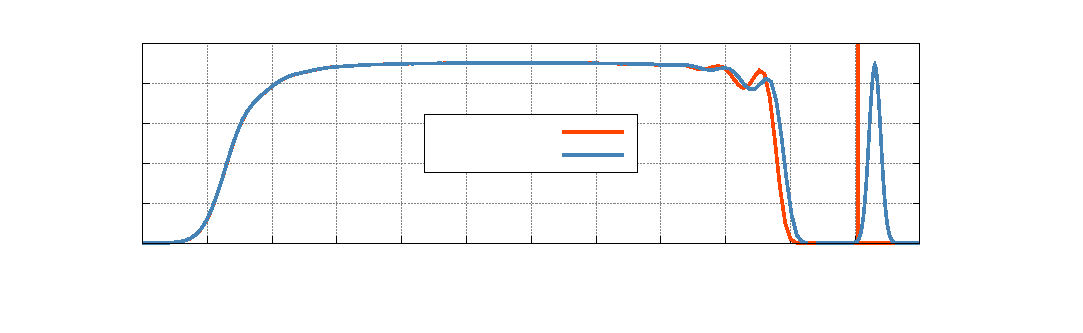
\includegraphics{4S-Q-C-lsolid}}%
    \gplfronttext
  \end{picture}%
\endgroup

	\vspace{-0.5\baselineskip}
	\caption{Density profile in a plane containing the center of mass of the droplet and the potassium atom, for a quantum or a classical description of K}
	\label{fig:4S-Q-C-lsolid}
\end{figure}

\subsection{Quick discussion on the influence of the version of the functional}

We already discussed the fact that the OTC functional could become unstable during a dynamics simulation due to the fact that it cannot handle sharp features appearing around attractive dopants. 
This can occur in the excited ($4p$) states because of the attractive $\Pi$ well. 
The two versions can be compared in the static study of the ground ($4s$) state.
We see in \citfig{fig:4S-C-otc-lsolid} that the two functionals give nearly the same helium density, except near the dopant where the solid version gives a smoother profile, as expected.
\begin{figure}[h]
	\centering
	% GNUPLOT: LaTeX picture with Postscript
\begingroup
  \makeatletter
  \providecommand\color[2][]{%
    \GenericError{(gnuplot) \space\space\space\@spaces}{%
      Package color not loaded in conjunction with
      terminal option `colourtext'%
    }{See the gnuplot documentation for explanation.%
    }{Either use 'blacktext' in gnuplot or load the package
      color.sty in LaTeX.}%
    \renewcommand\color[2][]{}%
  }%
  \providecommand\includegraphics[2][]{%
    \GenericError{(gnuplot) \space\space\space\@spaces}{%
      Package graphicx or graphics not loaded%
    }{See the gnuplot documentation for explanation.%
    }{The gnuplot epslatex terminal needs graphicx.sty or graphics.sty.}%
    \renewcommand\includegraphics[2][]{}%
  }%
  \providecommand\rotatebox[2]{#2}%
  \@ifundefined{ifGPcolor}{%
    \newif\ifGPcolor
    \GPcolortrue
  }{}%
  \@ifundefined{ifGPblacktext}{%
    \newif\ifGPblacktext
    \GPblacktextfalse
  }{}%
  % define a \g@addto@macro without @ in the name:
  \let\gplgaddtomacro\g@addto@macro
  % define empty templates for all commands taking text:
  \gdef\gplbacktext{}%
  \gdef\gplfronttext{}%
  \makeatother
  \ifGPblacktext
    % no textcolor at all
    \def\colorrgb#1{}%
    \def\colorgray#1{}%
  \else
    % gray or color?
    \ifGPcolor
      \def\colorrgb#1{\color[rgb]{#1}}%
      \def\colorgray#1{\color[gray]{#1}}%
      \expandafter\def\csname LTw\endcsname{\color{white}}%
      \expandafter\def\csname LTb\endcsname{\color{black}}%
      \expandafter\def\csname LTa\endcsname{\color{black}}%
      \expandafter\def\csname LT0\endcsname{\color[rgb]{1,0,0}}%
      \expandafter\def\csname LT1\endcsname{\color[rgb]{0,1,0}}%
      \expandafter\def\csname LT2\endcsname{\color[rgb]{0,0,1}}%
      \expandafter\def\csname LT3\endcsname{\color[rgb]{1,0,1}}%
      \expandafter\def\csname LT4\endcsname{\color[rgb]{0,1,1}}%
      \expandafter\def\csname LT5\endcsname{\color[rgb]{1,1,0}}%
      \expandafter\def\csname LT6\endcsname{\color[rgb]{0,0,0}}%
      \expandafter\def\csname LT7\endcsname{\color[rgb]{1,0.3,0}}%
      \expandafter\def\csname LT8\endcsname{\color[rgb]{0.5,0.5,0.5}}%
    \else
      % gray
      \def\colorrgb#1{\color{black}}%
      \def\colorgray#1{\color[gray]{#1}}%
      \expandafter\def\csname LTw\endcsname{\color{white}}%
      \expandafter\def\csname LTb\endcsname{\color{black}}%
      \expandafter\def\csname LTa\endcsname{\color{black}}%
      \expandafter\def\csname LT0\endcsname{\color{black}}%
      \expandafter\def\csname LT1\endcsname{\color{black}}%
      \expandafter\def\csname LT2\endcsname{\color{black}}%
      \expandafter\def\csname LT3\endcsname{\color{black}}%
      \expandafter\def\csname LT4\endcsname{\color{black}}%
      \expandafter\def\csname LT5\endcsname{\color{black}}%
      \expandafter\def\csname LT6\endcsname{\color{black}}%
      \expandafter\def\csname LT7\endcsname{\color{black}}%
      \expandafter\def\csname LT8\endcsname{\color{black}}%
    \fi
  \fi
    \setlength{\unitlength}{0.0500bp}%
    \ifx\gptboxheight\undefined%
      \newlength{\gptboxheight}%
      \newlength{\gptboxwidth}%
      \newsavebox{\gptboxtext}%
    \fi%
    \setlength{\fboxrule}{0.5pt}%
    \setlength{\fboxsep}{1pt}%
\begin{picture}(10080.00,2880.00)%
    \gplgaddtomacro\gplbacktext{%
      \csname LTb\endcsname%
      \put(1078,704){\makebox(0,0)[r]{\strut{}$0$}}%
      \csname LTb\endcsname%
      \put(1078,1086){\makebox(0,0)[r]{\strut{}$0.005$}}%
      \csname LTb\endcsname%
      \put(1078,1468){\makebox(0,0)[r]{\strut{}$0.01$}}%
      \csname LTb\endcsname%
      \put(1078,1851){\makebox(0,0)[r]{\strut{}$0.015$}}%
      \csname LTb\endcsname%
      \put(1078,2233){\makebox(0,0)[r]{\strut{}$0.02$}}%
      \csname LTb\endcsname%
      \put(1078,2615){\makebox(0,0)[r]{\strut{}$0.025$}}%
      \csname LTb\endcsname%
      \put(1210,484){\makebox(0,0){\strut{}$0$}}%
      \csname LTb\endcsname%
      \put(1916,484){\makebox(0,0){\strut{}$5$}}%
      \csname LTb\endcsname%
      \put(2622,484){\makebox(0,0){\strut{}$10$}}%
      \csname LTb\endcsname%
      \put(3328,484){\makebox(0,0){\strut{}$15$}}%
      \csname LTb\endcsname%
      \put(4034,484){\makebox(0,0){\strut{}$20$}}%
      \csname LTb\endcsname%
      \put(4740,484){\makebox(0,0){\strut{}$25$}}%
      \csname LTb\endcsname%
      \put(5447,484){\makebox(0,0){\strut{}$30$}}%
      \csname LTb\endcsname%
      \put(6153,484){\makebox(0,0){\strut{}$35$}}%
      \csname LTb\endcsname%
      \put(6859,484){\makebox(0,0){\strut{}$40$}}%
      \csname LTb\endcsname%
      \put(7565,484){\makebox(0,0){\strut{}$45$}}%
      \csname LTb\endcsname%
      \put(8271,484){\makebox(0,0){\strut{}$50$}}%
      \csname LTb\endcsname%
      \put(8977,484){\makebox(0,0){\strut{}$55$}}%
      \csname LTb\endcsname%
      \put(9683,484){\makebox(0,0){\strut{}$60$}}%
    }%
    \gplgaddtomacro\gplfronttext{%
      \csname LTb\endcsname%
      \put(176,1659){\rotatebox{-270}{\makebox(0,0){\strut{}Helium density (\AA$^{-3}$)}}}%
      \put(5446,154){\makebox(0,0){\strut{}Position (\AA)}}%
      \csname LTb\endcsname%
      \put(5349,1769){\makebox(0,0)[r]{\strut{}Solid}}%
      \csname LTb\endcsname%
      \put(5349,1549){\makebox(0,0)[r]{\strut{}OTC}}%
    }%
    \gplbacktext
    \put(0,0){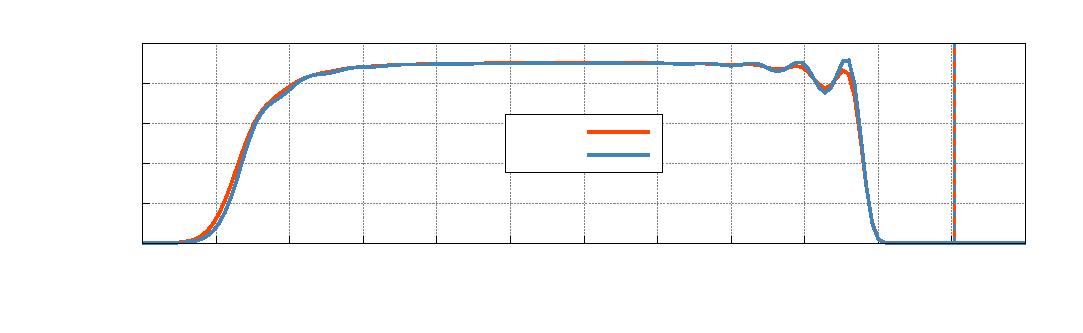
\includegraphics{4S-C-otc-lsolid}}%
    \gplfronttext
  \end{picture}%
\endgroup

	\vspace{-0.5\baselineskip}
	\caption{Density profile in a plane containing the center of mass of the droplet and the potassium atom, for the solid or the OTC functional}
	\label{fig:4S-C-otc-lsolid}
\end{figure}

\subsection{Justifying diabatic hypothesis}

One model that has been very much used to interpret experimental spectra of alkali atoms bound to helium droplets or even some of the dynamics aspects of their photodissociation is the so-called \emph{pseudo-diatomic model}.
In this model the system is represented as a diatomic molecule in which the helium droplet plays the role of a pseudo-atom.
The potential energy curves for this model are then taken by averaging the pair potentials over the (static) helium density. \\

There are two ways of choosing which density to use for this convolution.
The first one is what we call the \textit{diabatic} hypothesis: the motion of K is supposed to be much faster than the droplet one. 
The second one, which will be called \textit{adiabatic}, optimizes the helium density for each value of the position of the dopant, which is equivalent to assuming that the helium density can adapt instantly to a new position of the potassium.
We use here the simple case of the ground ($4s$) study to get an idea of which hypothesis is closer to reality.
Let us stress that both models imply that there is no energy exchange between the dopant and the droplet during the dynamics, whereas in the TDDFT description the whole dynamics is described, albeit in a mean-field way.\\

Our formalism (minimization of a functional with respect to all its parameters) makes it possible to add constraints to our minimization.
We can thus impose a given distance $\mathcal{Z}_0$ between the dopant and the helium center of mass (the actual distance is noted $\mathcal{Z}$)
\begin{align}
E[\rho]\rightarrow E[\rho,\mathcal{Z}_0] = E[\rho] + \frac{\alpha}{2}(\mathcal{Z}-\mathcal{Z}_0)^2 \quad \text{with $\alpha$ an arbitrary constant}
\end{align}

Then we proceed in the following way: we start simulations with different $\mathcal{Z}_0$ value and we register the first and last energy balance. 
The first one give the system energy without relaxation (diabatic approximation) while the final one gives the energy after minimization (adiabatic approximation). In order to decide which of the two approximations is better to describe our system we can compare the results to the DFT simulation with a quantum description of K, which is expected to be more accurate. 
The idea is to consider that in the ground state the particle is locally feeling a harmonic potential, so we can use the well known ground state wave function and associated energy.
\begin{align}
\psi_0(z) = \left(\frac{\alpha}{\pi}\right)^{1/4} \mathrm{e}^{-\alpha \, z^2/2} \quad \text{and} \quad E_0 = \frac{\hbar\omega}{2} \quad \text{with} \quad \alpha = \frac{m\omega}{\hbar}
\label{eq:4S-oh}
\end{align}

The results are shown in \citfig{fig:4S-potentials}.
First we can note that the diabatic and adiabatic potentials do not reach the same asymptotic energy.
This is because in the adiabatic approximation the helium droplet is a pure, relaxed helium droplet while in the diabatic one it has the same density as when the potassium was at equilibrium distance.
Second, we observe that the quantum case (DFT with quantum description of K) seems to be closer to the diabatic approximation. 

\begin{figure}[h]
\centering
    % GNUPLOT: LaTeX picture with Postscript
\begingroup
  \makeatletter
  \providecommand\color[2][]{%
    \GenericError{(gnuplot) \space\space\space\@spaces}{%
      Package color not loaded in conjunction with
      terminal option `colourtext'%
    }{See the gnuplot documentation for explanation.%
    }{Either use 'blacktext' in gnuplot or load the package
      color.sty in LaTeX.}%
    \renewcommand\color[2][]{}%
  }%
  \providecommand\includegraphics[2][]{%
    \GenericError{(gnuplot) \space\space\space\@spaces}{%
      Package graphicx or graphics not loaded%
    }{See the gnuplot documentation for explanation.%
    }{The gnuplot epslatex terminal needs graphicx.sty or graphics.sty.}%
    \renewcommand\includegraphics[2][]{}%
  }%
  \providecommand\rotatebox[2]{#2}%
  \@ifundefined{ifGPcolor}{%
    \newif\ifGPcolor
    \GPcolortrue
  }{}%
  \@ifundefined{ifGPblacktext}{%
    \newif\ifGPblacktext
    \GPblacktextfalse
  }{}%
  % define a \g@addto@macro without @ in the name:
  \let\gplgaddtomacro\g@addto@macro
  % define empty templates for all commands taking text:
  \gdef\gplbacktext{}%
  \gdef\gplfronttext{}%
  \makeatother
  \ifGPblacktext
    % no textcolor at all
    \def\colorrgb#1{}%
    \def\colorgray#1{}%
  \else
    % gray or color?
    \ifGPcolor
      \def\colorrgb#1{\color[rgb]{#1}}%
      \def\colorgray#1{\color[gray]{#1}}%
      \expandafter\def\csname LTw\endcsname{\color{white}}%
      \expandafter\def\csname LTb\endcsname{\color{black}}%
      \expandafter\def\csname LTa\endcsname{\color{black}}%
      \expandafter\def\csname LT0\endcsname{\color[rgb]{1,0,0}}%
      \expandafter\def\csname LT1\endcsname{\color[rgb]{0,1,0}}%
      \expandafter\def\csname LT2\endcsname{\color[rgb]{0,0,1}}%
      \expandafter\def\csname LT3\endcsname{\color[rgb]{1,0,1}}%
      \expandafter\def\csname LT4\endcsname{\color[rgb]{0,1,1}}%
      \expandafter\def\csname LT5\endcsname{\color[rgb]{1,1,0}}%
      \expandafter\def\csname LT6\endcsname{\color[rgb]{0,0,0}}%
      \expandafter\def\csname LT7\endcsname{\color[rgb]{1,0.3,0}}%
      \expandafter\def\csname LT8\endcsname{\color[rgb]{0.5,0.5,0.5}}%
    \else
      % gray
      \def\colorrgb#1{\color{black}}%
      \def\colorgray#1{\color[gray]{#1}}%
      \expandafter\def\csname LTw\endcsname{\color{white}}%
      \expandafter\def\csname LTb\endcsname{\color{black}}%
      \expandafter\def\csname LTa\endcsname{\color{black}}%
      \expandafter\def\csname LT0\endcsname{\color{black}}%
      \expandafter\def\csname LT1\endcsname{\color{black}}%
      \expandafter\def\csname LT2\endcsname{\color{black}}%
      \expandafter\def\csname LT3\endcsname{\color{black}}%
      \expandafter\def\csname LT4\endcsname{\color{black}}%
      \expandafter\def\csname LT5\endcsname{\color{black}}%
      \expandafter\def\csname LT6\endcsname{\color{black}}%
      \expandafter\def\csname LT7\endcsname{\color{black}}%
      \expandafter\def\csname LT8\endcsname{\color{black}}%
    \fi
  \fi
    \setlength{\unitlength}{0.0500bp}%
    \ifx\gptboxheight\undefined%
      \newlength{\gptboxheight}%
      \newlength{\gptboxwidth}%
      \newsavebox{\gptboxtext}%
    \fi%
    \setlength{\fboxrule}{0.5pt}%
    \setlength{\fboxsep}{1pt}%
\begin{picture}(10080.00,3600.00)%
    \gplgaddtomacro\gplbacktext{%
      \csname LTb\endcsname%
      \put(946,704){\makebox(0,0)[r]{\strut{}$-10$}}%
      \csname LTb\endcsname%
      \put(946,1080){\makebox(0,0)[r]{\strut{}$-7.5$}}%
      \csname LTb\endcsname%
      \put(946,1456){\makebox(0,0)[r]{\strut{}$-5$}}%
      \csname LTb\endcsname%
      \put(946,1832){\makebox(0,0)[r]{\strut{}$-2.5$}}%
      \csname LTb\endcsname%
      \put(946,2207){\makebox(0,0)[r]{\strut{}$0$}}%
      \csname LTb\endcsname%
      \put(946,2583){\makebox(0,0)[r]{\strut{}$2.5$}}%
      \csname LTb\endcsname%
      \put(946,2959){\makebox(0,0)[r]{\strut{}$5$}}%
      \csname LTb\endcsname%
      \put(946,3335){\makebox(0,0)[r]{\strut{}$7.5$}}%
      \csname LTb\endcsname%
      \put(1078,484){\makebox(0,0){\strut{}$-5$}}%
      \csname LTb\endcsname%
      \put(1740,484){\makebox(0,0){\strut{}$-4$}}%
      \csname LTb\endcsname%
      \put(2402,484){\makebox(0,0){\strut{}$-3$}}%
      \csname LTb\endcsname%
      \put(3064,484){\makebox(0,0){\strut{}$-2$}}%
      \csname LTb\endcsname%
      \put(3726,484){\makebox(0,0){\strut{}$-1$}}%
      \csname LTb\endcsname%
      \put(4388,484){\makebox(0,0){\strut{}$0$}}%
      \csname LTb\endcsname%
      \put(5050,484){\makebox(0,0){\strut{}$1$}}%
      \csname LTb\endcsname%
      \put(5711,484){\makebox(0,0){\strut{}$2$}}%
      \csname LTb\endcsname%
      \put(6373,484){\makebox(0,0){\strut{}$3$}}%
      \csname LTb\endcsname%
      \put(7035,484){\makebox(0,0){\strut{}$4$}}%
      \csname LTb\endcsname%
      \put(7697,484){\makebox(0,0){\strut{}$5$}}%
      \csname LTb\endcsname%
      \put(8359,484){\makebox(0,0){\strut{}$6$}}%
      \csname LTb\endcsname%
      \put(9021,484){\makebox(0,0){\strut{}$7$}}%
      \csname LTb\endcsname%
      \put(9683,484){\makebox(0,0){\strut{}$8$}}%
    }%
    \gplgaddtomacro\gplfronttext{%
      \csname LTb\endcsname%
      \put(176,2019){\rotatebox{-270}{\makebox(0,0){\strut{}Energy (K)}}}%
      \put(5380,154){\makebox(0,0){\strut{}Distance from equilibrium (\AA)}}%
      \csname LTb\endcsname%
      \put(8696,3107){\makebox(0,0)[r]{\strut{}Quantum}}%
      \csname LTb\endcsname%
      \put(8696,2887){\makebox(0,0)[r]{\strut{}Diabatic}}%
      \csname LTb\endcsname%
      \put(8696,2667){\makebox(0,0)[r]{\strut{}Adiabatic}}%
    }%
    \gplbacktext
    \put(0,0){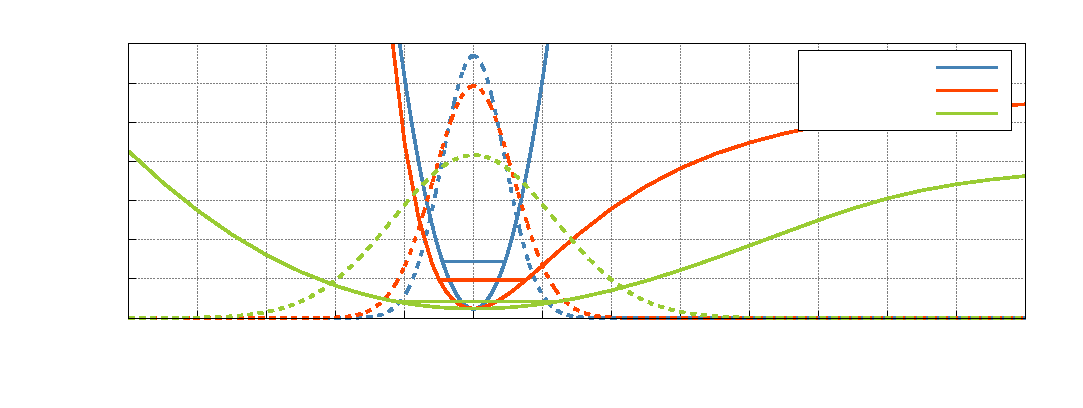
\includegraphics{4S-potentials}}%
    \gplfronttext
  \end{picture}%
\endgroup

    \vspace{-0.5\baselineskip}
    \caption{Diabatic, adiabatic and quantum potentials with associated wave functions and zero point energies in the harmonic approximation. The quantum potential is deduced from a harmonic fit of the wave function obtained from DFT with K treated quantum mechanically; the diabatic and adiabatic wave functions are obtained from a harmonic fit of the corresponding potentials}
    \label{fig:4S-potentials}
\end{figure}
\section{Classical dynamics towards ($4p$) states}

The ground state properties being established, we will now present the dynamics simulation of the KHe$_N$ system under a $4p\leftarrow 4s$ photo-excitation. 
As already discussed, the $4p$ state is split by interaction with helium and by spin-orbit coupling.
Hence we will present the dynamics following each of the three $\Pi_{1/2}$, $\Pi_{3/2}$ and $\Sigma_{1/2}$ excitations.

\subsection{Quantum versus classical spectra}
\label{sec:4P-spectra}

\begin{figure}[h!]
	\centering
	\begin{minipage}[c]{0.48\linewidth}
		% GNUPLOT: LaTeX picture with Postscript
\begingroup
  \makeatletter
  \providecommand\color[2][]{%
    \GenericError{(gnuplot) \space\space\space\@spaces}{%
      Package color not loaded in conjunction with
      terminal option `colourtext'%
    }{See the gnuplot documentation for explanation.%
    }{Either use 'blacktext' in gnuplot or load the package
      color.sty in LaTeX.}%
    \renewcommand\color[2][]{}%
  }%
  \providecommand\includegraphics[2][]{%
    \GenericError{(gnuplot) \space\space\space\@spaces}{%
      Package graphicx or graphics not loaded%
    }{See the gnuplot documentation for explanation.%
    }{The gnuplot epslatex terminal needs graphicx.sty or graphics.sty.}%
    \renewcommand\includegraphics[2][]{}%
  }%
  \providecommand\rotatebox[2]{#2}%
  \@ifundefined{ifGPcolor}{%
    \newif\ifGPcolor
    \GPcolortrue
  }{}%
  \@ifundefined{ifGPblacktext}{%
    \newif\ifGPblacktext
    \GPblacktextfalse
  }{}%
  % define a \g@addto@macro without @ in the name:
  \let\gplgaddtomacro\g@addto@macro
  % define empty templates for all commands taking text:
  \gdef\gplbacktext{}%
  \gdef\gplfronttext{}%
  \makeatother
  \ifGPblacktext
    % no textcolor at all
    \def\colorrgb#1{}%
    \def\colorgray#1{}%
  \else
    % gray or color?
    \ifGPcolor
      \def\colorrgb#1{\color[rgb]{#1}}%
      \def\colorgray#1{\color[gray]{#1}}%
      \expandafter\def\csname LTw\endcsname{\color{white}}%
      \expandafter\def\csname LTb\endcsname{\color{black}}%
      \expandafter\def\csname LTa\endcsname{\color{black}}%
      \expandafter\def\csname LT0\endcsname{\color[rgb]{1,0,0}}%
      \expandafter\def\csname LT1\endcsname{\color[rgb]{0,1,0}}%
      \expandafter\def\csname LT2\endcsname{\color[rgb]{0,0,1}}%
      \expandafter\def\csname LT3\endcsname{\color[rgb]{1,0,1}}%
      \expandafter\def\csname LT4\endcsname{\color[rgb]{0,1,1}}%
      \expandafter\def\csname LT5\endcsname{\color[rgb]{1,1,0}}%
      \expandafter\def\csname LT6\endcsname{\color[rgb]{0,0,0}}%
      \expandafter\def\csname LT7\endcsname{\color[rgb]{1,0.3,0}}%
      \expandafter\def\csname LT8\endcsname{\color[rgb]{0.5,0.5,0.5}}%
    \else
      % gray
      \def\colorrgb#1{\color{black}}%
      \def\colorgray#1{\color[gray]{#1}}%
      \expandafter\def\csname LTw\endcsname{\color{white}}%
      \expandafter\def\csname LTb\endcsname{\color{black}}%
      \expandafter\def\csname LTa\endcsname{\color{black}}%
      \expandafter\def\csname LT0\endcsname{\color{black}}%
      \expandafter\def\csname LT1\endcsname{\color{black}}%
      \expandafter\def\csname LT2\endcsname{\color{black}}%
      \expandafter\def\csname LT3\endcsname{\color{black}}%
      \expandafter\def\csname LT4\endcsname{\color{black}}%
      \expandafter\def\csname LT5\endcsname{\color{black}}%
      \expandafter\def\csname LT6\endcsname{\color{black}}%
      \expandafter\def\csname LT7\endcsname{\color{black}}%
      \expandafter\def\csname LT8\endcsname{\color{black}}%
    \fi
  \fi
    \setlength{\unitlength}{0.0500bp}%
    \ifx\gptboxheight\undefined%
      \newlength{\gptboxheight}%
      \newlength{\gptboxwidth}%
      \newsavebox{\gptboxtext}%
    \fi%
    \setlength{\fboxrule}{0.5pt}%
    \setlength{\fboxsep}{1pt}%
\begin{picture}(4752.00,2880.00)%
    \gplgaddtomacro\gplbacktext{%
      \csname LTb\endcsname%
      \put(708,432){\makebox(0,0)[r]{\strut{}$0$}}%
      \csname LTb\endcsname%
      \put(708,921){\makebox(0,0)[r]{\strut{}$0.2$}}%
      \csname LTb\endcsname%
      \put(708,1411){\makebox(0,0)[r]{\strut{}$0.4$}}%
      \csname LTb\endcsname%
      \put(708,1900){\makebox(0,0)[r]{\strut{}$0.6$}}%
      \csname LTb\endcsname%
      \put(708,2390){\makebox(0,0)[r]{\strut{}$0.8$}}%
      \csname LTb\endcsname%
      \put(708,2879){\makebox(0,0)[r]{\strut{}$1$}}%
      \csname LTb\endcsname%
      \put(1299,212){\makebox(0,0){\strut{}$13000$}}%
      \csname LTb\endcsname%
      \put(2217,212){\makebox(0,0){\strut{}$13100$}}%
      \csname LTb\endcsname%
      \put(3136,212){\makebox(0,0){\strut{}$13200$}}%
      \csname LTb\endcsname%
      \put(4054,212){\makebox(0,0){\strut{}$13300$}}%
    }%
    \gplgaddtomacro\gplfronttext{%
      \csname LTb\endcsname%
      \put(176,1655){\rotatebox{-270}{\makebox(0,0){\strut{}Intensity (arb. unit)}}}%
      \put(2676,-74){\makebox(0,0){\strut{}Energy (cm$^{-1}$)}}%
      \csname LTb\endcsname%
      \put(3526,2651){\makebox(0,0)[r]{\strut{}$\Sigma_{1/2}$}}%
      \csname LTb\endcsname%
      \put(3526,2431){\makebox(0,0)[r]{\strut{}$\Pi_{3/2}$}}%
      \csname LTb\endcsname%
      \put(3526,2211){\makebox(0,0)[r]{\strut{}$\Pi_{1/2}$}}%
    }%
    \gplbacktext
    \put(0,0){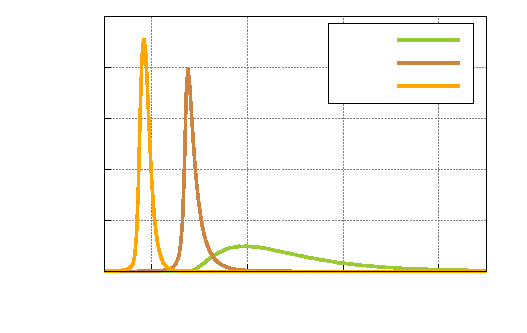
\includegraphics{4P-sp-Q}}%
    \gplfronttext
  \end{picture}%
\endgroup

		\label{fig:4P-sp-Q}
		\vspace{0.2\baselineskip}
		\caption{$4p\rightarrow 4s$ absorption spectra with different state contributions for quantum K}
	\end{minipage}
\hfill
	\begin{minipage}[c]{0.48\linewidth}
		% GNUPLOT: LaTeX picture with Postscript
\begingroup
  \makeatletter
  \providecommand\color[2][]{%
    \GenericError{(gnuplot) \space\space\space\@spaces}{%
      Package color not loaded in conjunction with
      terminal option `colourtext'%
    }{See the gnuplot documentation for explanation.%
    }{Either use 'blacktext' in gnuplot or load the package
      color.sty in LaTeX.}%
    \renewcommand\color[2][]{}%
  }%
  \providecommand\includegraphics[2][]{%
    \GenericError{(gnuplot) \space\space\space\@spaces}{%
      Package graphicx or graphics not loaded%
    }{See the gnuplot documentation for explanation.%
    }{The gnuplot epslatex terminal needs graphicx.sty or graphics.sty.}%
    \renewcommand\includegraphics[2][]{}%
  }%
  \providecommand\rotatebox[2]{#2}%
  \@ifundefined{ifGPcolor}{%
    \newif\ifGPcolor
    \GPcolortrue
  }{}%
  \@ifundefined{ifGPblacktext}{%
    \newif\ifGPblacktext
    \GPblacktextfalse
  }{}%
  % define a \g@addto@macro without @ in the name:
  \let\gplgaddtomacro\g@addto@macro
  % define empty templates for all commands taking text:
  \gdef\gplbacktext{}%
  \gdef\gplfronttext{}%
  \makeatother
  \ifGPblacktext
    % no textcolor at all
    \def\colorrgb#1{}%
    \def\colorgray#1{}%
  \else
    % gray or color?
    \ifGPcolor
      \def\colorrgb#1{\color[rgb]{#1}}%
      \def\colorgray#1{\color[gray]{#1}}%
      \expandafter\def\csname LTw\endcsname{\color{white}}%
      \expandafter\def\csname LTb\endcsname{\color{black}}%
      \expandafter\def\csname LTa\endcsname{\color{black}}%
      \expandafter\def\csname LT0\endcsname{\color[rgb]{1,0,0}}%
      \expandafter\def\csname LT1\endcsname{\color[rgb]{0,1,0}}%
      \expandafter\def\csname LT2\endcsname{\color[rgb]{0,0,1}}%
      \expandafter\def\csname LT3\endcsname{\color[rgb]{1,0,1}}%
      \expandafter\def\csname LT4\endcsname{\color[rgb]{0,1,1}}%
      \expandafter\def\csname LT5\endcsname{\color[rgb]{1,1,0}}%
      \expandafter\def\csname LT6\endcsname{\color[rgb]{0,0,0}}%
      \expandafter\def\csname LT7\endcsname{\color[rgb]{1,0.3,0}}%
      \expandafter\def\csname LT8\endcsname{\color[rgb]{0.5,0.5,0.5}}%
    \else
      % gray
      \def\colorrgb#1{\color{black}}%
      \def\colorgray#1{\color[gray]{#1}}%
      \expandafter\def\csname LTw\endcsname{\color{white}}%
      \expandafter\def\csname LTb\endcsname{\color{black}}%
      \expandafter\def\csname LTa\endcsname{\color{black}}%
      \expandafter\def\csname LT0\endcsname{\color{black}}%
      \expandafter\def\csname LT1\endcsname{\color{black}}%
      \expandafter\def\csname LT2\endcsname{\color{black}}%
      \expandafter\def\csname LT3\endcsname{\color{black}}%
      \expandafter\def\csname LT4\endcsname{\color{black}}%
      \expandafter\def\csname LT5\endcsname{\color{black}}%
      \expandafter\def\csname LT6\endcsname{\color{black}}%
      \expandafter\def\csname LT7\endcsname{\color{black}}%
      \expandafter\def\csname LT8\endcsname{\color{black}}%
    \fi
  \fi
    \setlength{\unitlength}{0.0500bp}%
    \ifx\gptboxheight\undefined%
      \newlength{\gptboxheight}%
      \newlength{\gptboxwidth}%
      \newsavebox{\gptboxtext}%
    \fi%
    \setlength{\fboxrule}{0.5pt}%
    \setlength{\fboxsep}{1pt}%
\begin{picture}(4752.00,2880.00)%
    \gplgaddtomacro\gplbacktext{%
      \csname LTb\endcsname%
      \put(708,432){\makebox(0,0)[r]{\strut{}$0$}}%
      \csname LTb\endcsname%
      \put(708,921){\makebox(0,0)[r]{\strut{}$0.2$}}%
      \csname LTb\endcsname%
      \put(708,1411){\makebox(0,0)[r]{\strut{}$0.4$}}%
      \csname LTb\endcsname%
      \put(708,1900){\makebox(0,0)[r]{\strut{}$0.6$}}%
      \csname LTb\endcsname%
      \put(708,2390){\makebox(0,0)[r]{\strut{}$0.8$}}%
      \csname LTb\endcsname%
      \put(708,2879){\makebox(0,0)[r]{\strut{}$1$}}%
      \csname LTb\endcsname%
      \put(1299,212){\makebox(0,0){\strut{}$13000$}}%
      \csname LTb\endcsname%
      \put(2217,212){\makebox(0,0){\strut{}$13100$}}%
      \csname LTb\endcsname%
      \put(3136,212){\makebox(0,0){\strut{}$13200$}}%
      \csname LTb\endcsname%
      \put(4054,212){\makebox(0,0){\strut{}$13300$}}%
    }%
    \gplgaddtomacro\gplfronttext{%
      \csname LTb\endcsname%
      \put(176,1655){\rotatebox{-270}{\makebox(0,0){\strut{}Intensity (arb. unit)}}}%
      \put(2676,-74){\makebox(0,0){\strut{}Energy (cm$^{-1}$)}}%
      \csname LTb\endcsname%
      \put(3526,2651){\makebox(0,0)[r]{\strut{}Classical}}%
      \csname LTb\endcsname%
      \put(3526,2431){\makebox(0,0)[r]{\strut{}Quantum}}%
      \csname LTb\endcsname%
      \put(3526,2211){\makebox(0,0)[r]{\strut{}Experiment}}%
    }%
    \gplbacktext
    \put(0,0){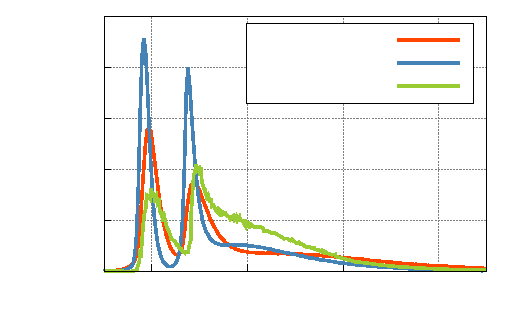
\includegraphics{4P-sp-QC}}%
    \gplfronttext
  \end{picture}%
\endgroup

		\label{fig:4P-sp-QC}
		\vspace{0.2\baselineskip}
		\caption{Comparisons between quantum, classical and experimental spectra \cite{Sti1996}}
	\end{minipage}
\end{figure}

The programs are not yet prepared to describe the quantum motion of K in an anisotropic state.
However, we can still use the quantum ground state density to simulate the spectra with the method described in the  \citanx{sec:ANX-spectra}.
This gives the only opportunity to judge the classical hypothesis for K motion by comparing this spectra to experimental data from \cite{Sti1996}.\\

We clearly see that both the classical and the quantum spectra give a very good agreement.
However,  they fail to describe the relative intensity of the two main peaks and they underestimate the $\Sigma_{1/2}$ component. 
We can conclude that the classical spectrum is really close to the quantum one and to the experimental data, which justifies our hypothesis and validates the potentials used.

\subsection{$\Sigma_{1/2}$ excitation: leaving free potassium}

\begin{figure}[h!]
	\begin{minipage}[c]{0.48\linewidth}
	\hspace{\oldindent} We start our dynamics study with the $\Sigma_{1/2}$ excitation. 
	We observe in \citfig{fig:4P-s12-pos} a fast ejection of the K atom in approximatively 0.2 ps. This behavior could be predicted from \citfig{fig:DIM-4p-pot}, because the averaged interaction is repulsive, however we have to be cautious because this only gives a snapshot of the energy profile at $t=0$ since the droplet is not rigid and can absorb energy from K.\\
	
	 \hspace{\oldindent} We note in \citfig{fig:4P-s12-snap} the global deformation of the droplet during ejection and the creation of density waves in the droplet.\\
	\end{minipage}
\hfill
	\begin{minipage}[c]{0.48\linewidth}
		\fbox{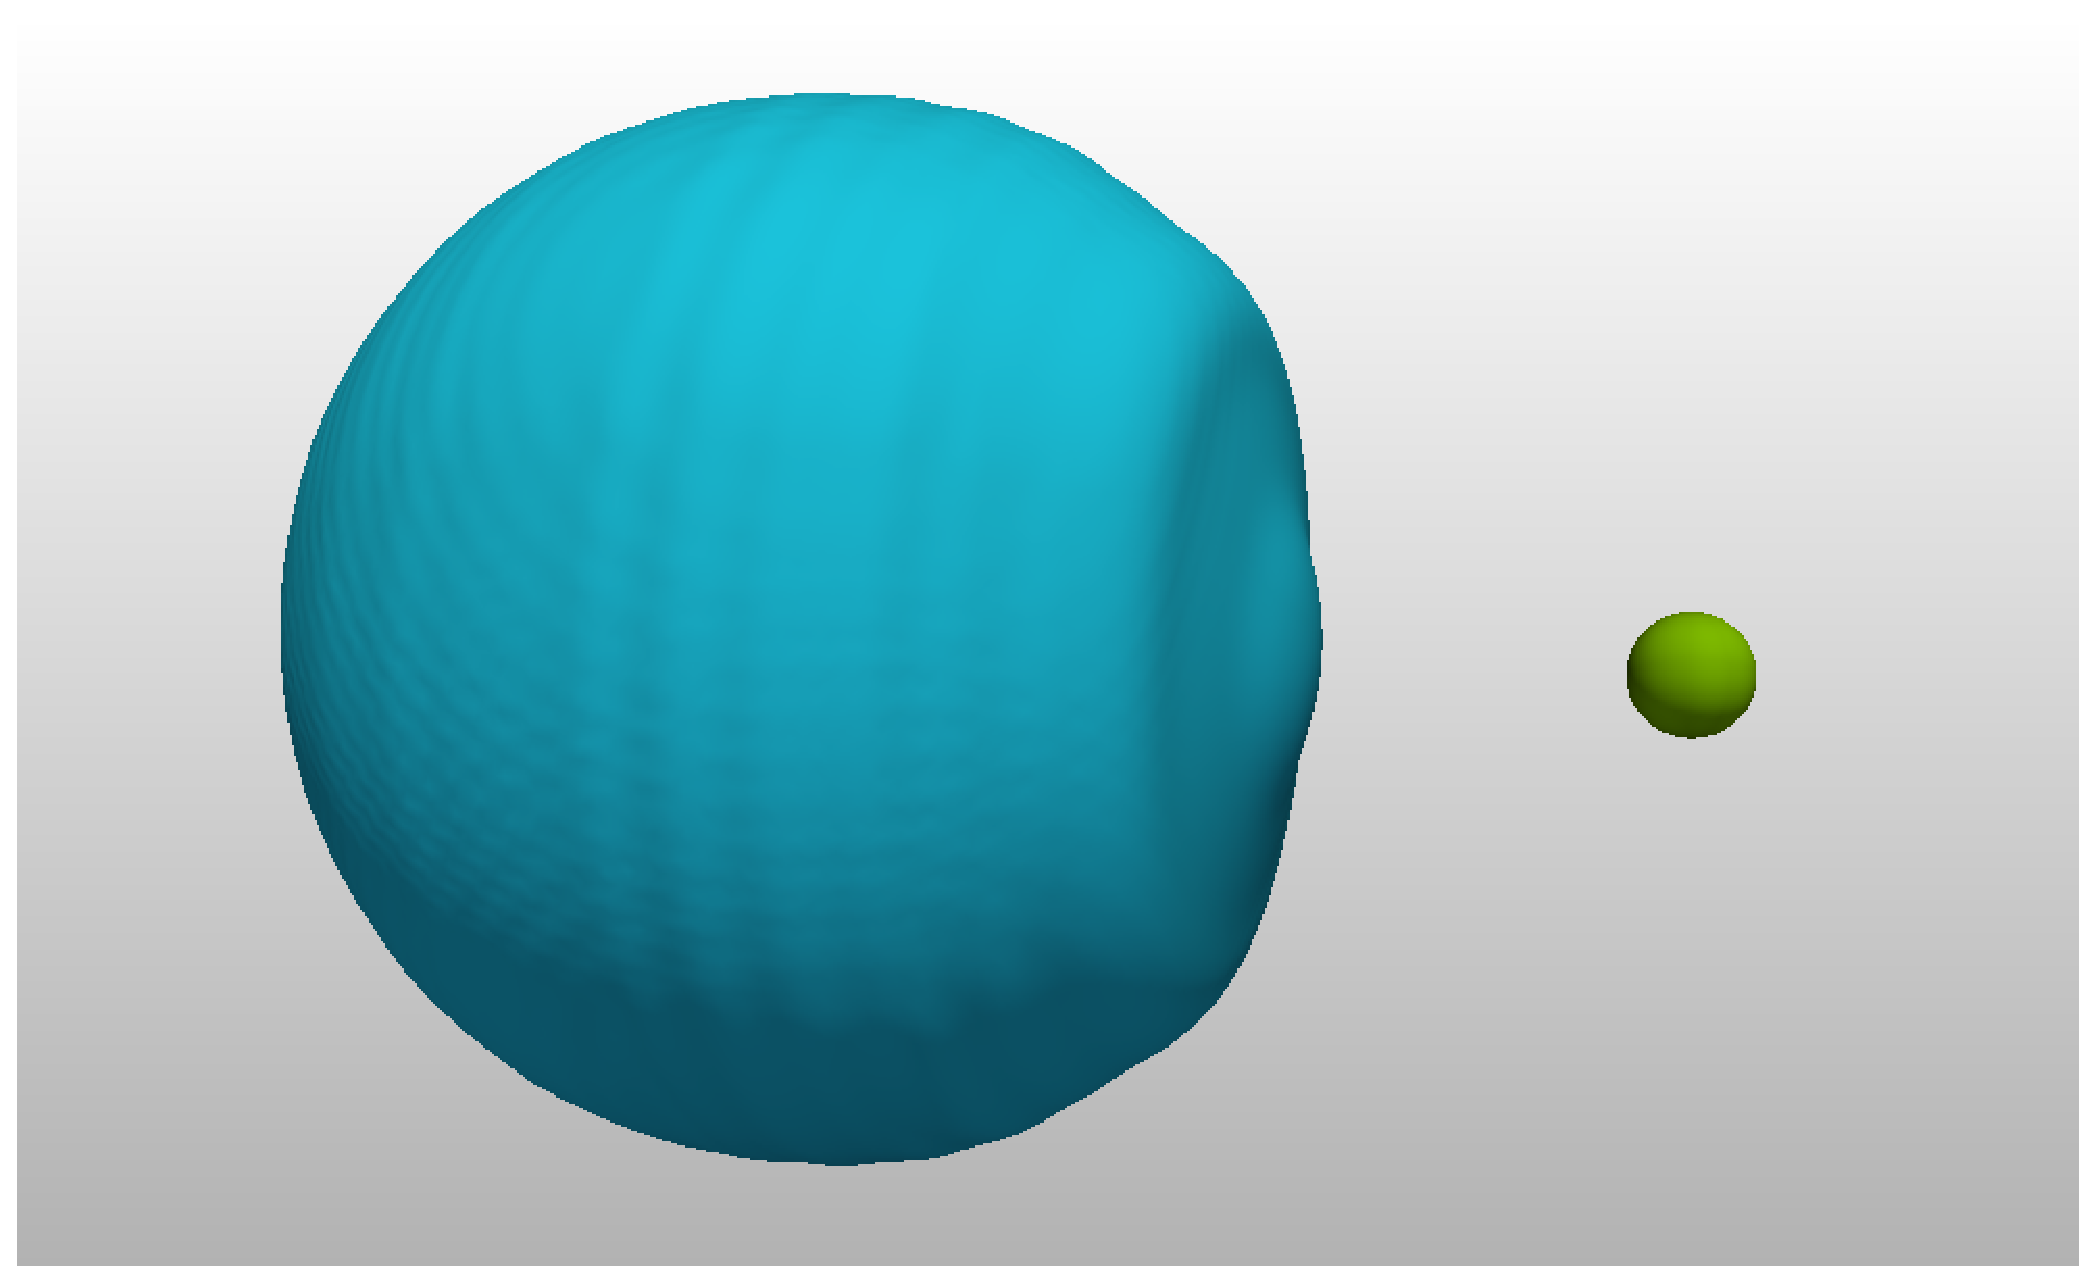
\includegraphics[scale=0.234]{4P-s12-snap}}
		\caption{Snapshot of He$_N$ density and leaving K at $t=8.5$ ps\label{fig:4P-s12-snap}}
	\end{minipage}
\end{figure}

\begin{figure}[h!]
	\centering
	\begin{minipage}[c]{0.48\linewidth}
		% GNUPLOT: LaTeX picture with Postscript
\begingroup
  \makeatletter
  \providecommand\color[2][]{%
    \GenericError{(gnuplot) \space\space\space\@spaces}{%
      Package color not loaded in conjunction with
      terminal option `colourtext'%
    }{See the gnuplot documentation for explanation.%
    }{Either use 'blacktext' in gnuplot or load the package
      color.sty in LaTeX.}%
    \renewcommand\color[2][]{}%
  }%
  \providecommand\includegraphics[2][]{%
    \GenericError{(gnuplot) \space\space\space\@spaces}{%
      Package graphicx or graphics not loaded%
    }{See the gnuplot documentation for explanation.%
    }{The gnuplot epslatex terminal needs graphicx.sty or graphics.sty.}%
    \renewcommand\includegraphics[2][]{}%
  }%
  \providecommand\rotatebox[2]{#2}%
  \@ifundefined{ifGPcolor}{%
    \newif\ifGPcolor
    \GPcolortrue
  }{}%
  \@ifundefined{ifGPblacktext}{%
    \newif\ifGPblacktext
    \GPblacktextfalse
  }{}%
  % define a \g@addto@macro without @ in the name:
  \let\gplgaddtomacro\g@addto@macro
  % define empty templates for all commands taking text:
  \gdef\gplbacktext{}%
  \gdef\gplfronttext{}%
  \makeatother
  \ifGPblacktext
    % no textcolor at all
    \def\colorrgb#1{}%
    \def\colorgray#1{}%
  \else
    % gray or color?
    \ifGPcolor
      \def\colorrgb#1{\color[rgb]{#1}}%
      \def\colorgray#1{\color[gray]{#1}}%
      \expandafter\def\csname LTw\endcsname{\color{white}}%
      \expandafter\def\csname LTb\endcsname{\color{black}}%
      \expandafter\def\csname LTa\endcsname{\color{black}}%
      \expandafter\def\csname LT0\endcsname{\color[rgb]{1,0,0}}%
      \expandafter\def\csname LT1\endcsname{\color[rgb]{0,1,0}}%
      \expandafter\def\csname LT2\endcsname{\color[rgb]{0,0,1}}%
      \expandafter\def\csname LT3\endcsname{\color[rgb]{1,0,1}}%
      \expandafter\def\csname LT4\endcsname{\color[rgb]{0,1,1}}%
      \expandafter\def\csname LT5\endcsname{\color[rgb]{1,1,0}}%
      \expandafter\def\csname LT6\endcsname{\color[rgb]{0,0,0}}%
      \expandafter\def\csname LT7\endcsname{\color[rgb]{1,0.3,0}}%
      \expandafter\def\csname LT8\endcsname{\color[rgb]{0.5,0.5,0.5}}%
    \else
      % gray
      \def\colorrgb#1{\color{black}}%
      \def\colorgray#1{\color[gray]{#1}}%
      \expandafter\def\csname LTw\endcsname{\color{white}}%
      \expandafter\def\csname LTb\endcsname{\color{black}}%
      \expandafter\def\csname LTa\endcsname{\color{black}}%
      \expandafter\def\csname LT0\endcsname{\color{black}}%
      \expandafter\def\csname LT1\endcsname{\color{black}}%
      \expandafter\def\csname LT2\endcsname{\color{black}}%
      \expandafter\def\csname LT3\endcsname{\color{black}}%
      \expandafter\def\csname LT4\endcsname{\color{black}}%
      \expandafter\def\csname LT5\endcsname{\color{black}}%
      \expandafter\def\csname LT6\endcsname{\color{black}}%
      \expandafter\def\csname LT7\endcsname{\color{black}}%
      \expandafter\def\csname LT8\endcsname{\color{black}}%
    \fi
  \fi
    \setlength{\unitlength}{0.0500bp}%
    \ifx\gptboxheight\undefined%
      \newlength{\gptboxheight}%
      \newlength{\gptboxwidth}%
      \newsavebox{\gptboxtext}%
    \fi%
    \setlength{\fboxrule}{0.5pt}%
    \setlength{\fboxsep}{1pt}%
\begin{picture}(4752.00,2880.00)%
    \gplgaddtomacro\gplbacktext{%
      \csname LTb\endcsname%
      \put(708,432){\makebox(0,0)[r]{\strut{}$0$}}%
      \csname LTb\endcsname%
      \put(708,921){\makebox(0,0)[r]{\strut{}$0.2$}}%
      \csname LTb\endcsname%
      \put(708,1411){\makebox(0,0)[r]{\strut{}$0.4$}}%
      \csname LTb\endcsname%
      \put(708,1900){\makebox(0,0)[r]{\strut{}$0.6$}}%
      \csname LTb\endcsname%
      \put(708,2390){\makebox(0,0)[r]{\strut{}$0.8$}}%
      \csname LTb\endcsname%
      \put(708,2879){\makebox(0,0)[r]{\strut{}$1$}}%
      \csname LTb\endcsname%
      \put(840,212){\makebox(0,0){\strut{}$0$}}%
      \csname LTb\endcsname%
      \put(1452,212){\makebox(0,0){\strut{}$2$}}%
      \csname LTb\endcsname%
      \put(2064,212){\makebox(0,0){\strut{}$4$}}%
      \csname LTb\endcsname%
      \put(2677,212){\makebox(0,0){\strut{}$6$}}%
      \csname LTb\endcsname%
      \put(3289,212){\makebox(0,0){\strut{}$8$}}%
      \csname LTb\endcsname%
      \put(3901,212){\makebox(0,0){\strut{}$10$}}%
      \csname LTb\endcsname%
      \put(4513,212){\makebox(0,0){\strut{}$12$}}%
    }%
    \gplgaddtomacro\gplfronttext{%
      \csname LTb\endcsname%
      \put(176,1655){\rotatebox{-270}{\makebox(0,0){\strut{}$|\langle p, s|\lambda\rangle|^2$}}}%
      \put(2676,-74){\makebox(0,0){\strut{}Time (ps)}}%
      \csname LTb\endcsname%
      \put(2837,1766){\makebox(0,0)[r]{\strut{}$\langle p_{1},- |$}}%
      \csname LTb\endcsname%
      \put(2837,1546){\makebox(0,0)[r]{\strut{}$\langle p_{0},+ |$}}%
    }%
    \gplbacktext
    \put(0,0){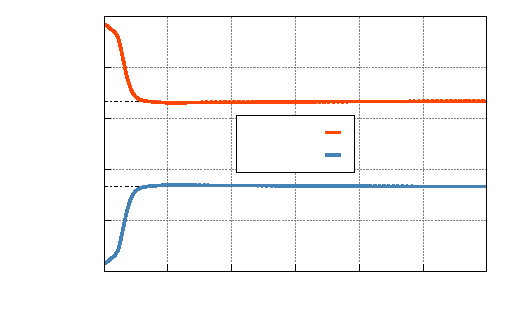
\includegraphics{4P-s12-proj}}%
    \gplfronttext
  \end{picture}%
\endgroup

		\vspace{0.2\baselineskip}
		\caption{Evolution of the electronic state as a function of time\label{fig:4P-s12-proj}}
	\end{minipage}
\hfill
	\begin{minipage}[c]{0.48\linewidth}
		% GNUPLOT: LaTeX picture with Postscript
\begingroup
  \makeatletter
  \providecommand\color[2][]{%
    \GenericError{(gnuplot) \space\space\space\@spaces}{%
      Package color not loaded in conjunction with
      terminal option `colourtext'%
    }{See the gnuplot documentation for explanation.%
    }{Either use 'blacktext' in gnuplot or load the package
      color.sty in LaTeX.}%
    \renewcommand\color[2][]{}%
  }%
  \providecommand\includegraphics[2][]{%
    \GenericError{(gnuplot) \space\space\space\@spaces}{%
      Package graphicx or graphics not loaded%
    }{See the gnuplot documentation for explanation.%
    }{The gnuplot epslatex terminal needs graphicx.sty or graphics.sty.}%
    \renewcommand\includegraphics[2][]{}%
  }%
  \providecommand\rotatebox[2]{#2}%
  \@ifundefined{ifGPcolor}{%
    \newif\ifGPcolor
    \GPcolortrue
  }{}%
  \@ifundefined{ifGPblacktext}{%
    \newif\ifGPblacktext
    \GPblacktextfalse
  }{}%
  % define a \g@addto@macro without @ in the name:
  \let\gplgaddtomacro\g@addto@macro
  % define empty templates for all commands taking text:
  \gdef\gplbacktext{}%
  \gdef\gplfronttext{}%
  \makeatother
  \ifGPblacktext
    % no textcolor at all
    \def\colorrgb#1{}%
    \def\colorgray#1{}%
  \else
    % gray or color?
    \ifGPcolor
      \def\colorrgb#1{\color[rgb]{#1}}%
      \def\colorgray#1{\color[gray]{#1}}%
      \expandafter\def\csname LTw\endcsname{\color{white}}%
      \expandafter\def\csname LTb\endcsname{\color{black}}%
      \expandafter\def\csname LTa\endcsname{\color{black}}%
      \expandafter\def\csname LT0\endcsname{\color[rgb]{1,0,0}}%
      \expandafter\def\csname LT1\endcsname{\color[rgb]{0,1,0}}%
      \expandafter\def\csname LT2\endcsname{\color[rgb]{0,0,1}}%
      \expandafter\def\csname LT3\endcsname{\color[rgb]{1,0,1}}%
      \expandafter\def\csname LT4\endcsname{\color[rgb]{0,1,1}}%
      \expandafter\def\csname LT5\endcsname{\color[rgb]{1,1,0}}%
      \expandafter\def\csname LT6\endcsname{\color[rgb]{0,0,0}}%
      \expandafter\def\csname LT7\endcsname{\color[rgb]{1,0.3,0}}%
      \expandafter\def\csname LT8\endcsname{\color[rgb]{0.5,0.5,0.5}}%
    \else
      % gray
      \def\colorrgb#1{\color{black}}%
      \def\colorgray#1{\color[gray]{#1}}%
      \expandafter\def\csname LTw\endcsname{\color{white}}%
      \expandafter\def\csname LTb\endcsname{\color{black}}%
      \expandafter\def\csname LTa\endcsname{\color{black}}%
      \expandafter\def\csname LT0\endcsname{\color{black}}%
      \expandafter\def\csname LT1\endcsname{\color{black}}%
      \expandafter\def\csname LT2\endcsname{\color{black}}%
      \expandafter\def\csname LT3\endcsname{\color{black}}%
      \expandafter\def\csname LT4\endcsname{\color{black}}%
      \expandafter\def\csname LT5\endcsname{\color{black}}%
      \expandafter\def\csname LT6\endcsname{\color{black}}%
      \expandafter\def\csname LT7\endcsname{\color{black}}%
      \expandafter\def\csname LT8\endcsname{\color{black}}%
    \fi
  \fi
    \setlength{\unitlength}{0.0500bp}%
    \ifx\gptboxheight\undefined%
      \newlength{\gptboxheight}%
      \newlength{\gptboxwidth}%
      \newsavebox{\gptboxtext}%
    \fi%
    \setlength{\fboxrule}{0.5pt}%
    \setlength{\fboxsep}{1pt}%
\begin{picture}(4752.00,2880.00)%
    \gplgaddtomacro\gplbacktext{%
      \csname LTb\endcsname%
      \put(946,432){\makebox(0,0)[r]{\strut{}$26.1$}}%
      \csname LTb\endcsname%
      \put(946,921){\makebox(0,0)[r]{\strut{}$26.4$}}%
      \csname LTb\endcsname%
      \put(946,1411){\makebox(0,0)[r]{\strut{}$26.7$}}%
      \csname LTb\endcsname%
      \put(946,1900){\makebox(0,0)[r]{\strut{}$27$}}%
      \csname LTb\endcsname%
      \put(946,2390){\makebox(0,0)[r]{\strut{}$27.3$}}%
      \csname LTb\endcsname%
      \put(946,2879){\makebox(0,0)[r]{\strut{}$27.6$}}%
      \csname LTb\endcsname%
      \put(1078,212){\makebox(0,0){\strut{}$0$}}%
      \csname LTb\endcsname%
      \put(1651,212){\makebox(0,0){\strut{}$0.2$}}%
      \csname LTb\endcsname%
      \put(2223,212){\makebox(0,0){\strut{}$0.4$}}%
      \csname LTb\endcsname%
      \put(2796,212){\makebox(0,0){\strut{}$0.6$}}%
      \csname LTb\endcsname%
      \put(3368,212){\makebox(0,0){\strut{}$0.8$}}%
      \csname LTb\endcsname%
      \put(3941,212){\makebox(0,0){\strut{}$1$}}%
      \csname LTb\endcsname%
      \put(4513,212){\makebox(0,0){\strut{}$1.2$}}%
    }%
    \gplgaddtomacro\gplfronttext{%
      \csname LTb\endcsname%
      \put(176,1655){\rotatebox{-270}{\makebox(0,0){\strut{}K relative position (\AA)}}}%
      \put(2795,-74){\makebox(0,0){\strut{}Time (ps)}}%
    }%
    \gplbacktext
    \put(0,0){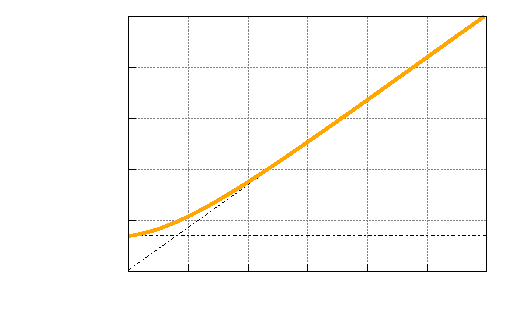
\includegraphics{4P-s12-pos}}%
    \gplfronttext
  \end{picture}%
\endgroup

		\vspace{0.2\baselineskip}
		\caption{Distance between K and He$_N$ centers of mass as a function of time\label{fig:4P-s12-pos}}
	\end{minipage}
\end{figure}

The study of the evolution of the internal electronic state will be important in following discussions, this is why we start discussing it for $\Sigma_{1/2}$ as a simple case. 
We saw in \citsec{sec:DIM-dia} that $\Omega$ is the only true good quantum number.
Here we have $\Omega=1/2$\footnote{We only discuss the positive case but the reasoning is the same for $\Omega=-1/2$ since they are degenerate}.
This can be checked in \citfig{fig:4P-s12-proj} since it is a linear combination of $\ket{p_1,-}$ and $\ket{p_0,+}$.
In addition we have seen that $\Lambda$ should be a good quantum number in the excitation region (\citsec{sec:DIM-dia}).
For the  $\Sigma_{1/2}$  state $\Lambda\approx 0$, which is why $\ket{p_0,+}$ is dominant at $t=0$.
Finally we can see that once K is far from droplet, its internal state becomes an eigenvector of $\vb{J}^2$ with eigenvalue $J=3/2$.
This is also expected because $J$ is a good quantum number in this region and the  $\Sigma_{1/2}$ state connects asymptotically to $J=3/2$  (\citsec{sec:DIM-4p})
\begin{align}
\ket{\lambda} \underset{t\rightarrow \infty}{\longrightarrow} \ket{J=3/2,\Omega=1/2} = \sqrt{\frac{1}{3}} \ket{p_1,-} + \sqrt{\frac{2}{3}} \ket{p_0,+}
\end{align}

\subsection{$\Pi_{1/2}$ excitation: complexity arises}

\subsubsection{Bouncing potassium}

\begin{figure}[h!]
	\centering
	\begin{minipage}[c]{0.48\linewidth}
		% GNUPLOT: LaTeX picture with Postscript
\begingroup
  \makeatletter
  \providecommand\color[2][]{%
    \GenericError{(gnuplot) \space\space\space\@spaces}{%
      Package color not loaded in conjunction with
      terminal option `colourtext'%
    }{See the gnuplot documentation for explanation.%
    }{Either use 'blacktext' in gnuplot or load the package
      color.sty in LaTeX.}%
    \renewcommand\color[2][]{}%
  }%
  \providecommand\includegraphics[2][]{%
    \GenericError{(gnuplot) \space\space\space\@spaces}{%
      Package graphicx or graphics not loaded%
    }{See the gnuplot documentation for explanation.%
    }{The gnuplot epslatex terminal needs graphicx.sty or graphics.sty.}%
    \renewcommand\includegraphics[2][]{}%
  }%
  \providecommand\rotatebox[2]{#2}%
  \@ifundefined{ifGPcolor}{%
    \newif\ifGPcolor
    \GPcolortrue
  }{}%
  \@ifundefined{ifGPblacktext}{%
    \newif\ifGPblacktext
    \GPblacktextfalse
  }{}%
  % define a \g@addto@macro without @ in the name:
  \let\gplgaddtomacro\g@addto@macro
  % define empty templates for all commands taking text:
  \gdef\gplbacktext{}%
  \gdef\gplfronttext{}%
  \makeatother
  \ifGPblacktext
    % no textcolor at all
    \def\colorrgb#1{}%
    \def\colorgray#1{}%
  \else
    % gray or color?
    \ifGPcolor
      \def\colorrgb#1{\color[rgb]{#1}}%
      \def\colorgray#1{\color[gray]{#1}}%
      \expandafter\def\csname LTw\endcsname{\color{white}}%
      \expandafter\def\csname LTb\endcsname{\color{black}}%
      \expandafter\def\csname LTa\endcsname{\color{black}}%
      \expandafter\def\csname LT0\endcsname{\color[rgb]{1,0,0}}%
      \expandafter\def\csname LT1\endcsname{\color[rgb]{0,1,0}}%
      \expandafter\def\csname LT2\endcsname{\color[rgb]{0,0,1}}%
      \expandafter\def\csname LT3\endcsname{\color[rgb]{1,0,1}}%
      \expandafter\def\csname LT4\endcsname{\color[rgb]{0,1,1}}%
      \expandafter\def\csname LT5\endcsname{\color[rgb]{1,1,0}}%
      \expandafter\def\csname LT6\endcsname{\color[rgb]{0,0,0}}%
      \expandafter\def\csname LT7\endcsname{\color[rgb]{1,0.3,0}}%
      \expandafter\def\csname LT8\endcsname{\color[rgb]{0.5,0.5,0.5}}%
    \else
      % gray
      \def\colorrgb#1{\color{black}}%
      \def\colorgray#1{\color[gray]{#1}}%
      \expandafter\def\csname LTw\endcsname{\color{white}}%
      \expandafter\def\csname LTb\endcsname{\color{black}}%
      \expandafter\def\csname LTa\endcsname{\color{black}}%
      \expandafter\def\csname LT0\endcsname{\color{black}}%
      \expandafter\def\csname LT1\endcsname{\color{black}}%
      \expandafter\def\csname LT2\endcsname{\color{black}}%
      \expandafter\def\csname LT3\endcsname{\color{black}}%
      \expandafter\def\csname LT4\endcsname{\color{black}}%
      \expandafter\def\csname LT5\endcsname{\color{black}}%
      \expandafter\def\csname LT6\endcsname{\color{black}}%
      \expandafter\def\csname LT7\endcsname{\color{black}}%
      \expandafter\def\csname LT8\endcsname{\color{black}}%
    \fi
  \fi
    \setlength{\unitlength}{0.0500bp}%
    \ifx\gptboxheight\undefined%
      \newlength{\gptboxheight}%
      \newlength{\gptboxwidth}%
      \newsavebox{\gptboxtext}%
    \fi%
    \setlength{\fboxrule}{0.5pt}%
    \setlength{\fboxsep}{1pt}%
\begin{picture}(4752.00,2880.00)%
    \gplgaddtomacro\gplbacktext{%
      \csname LTb\endcsname%
      \put(682,432){\makebox(0,0)[r]{\strut{}$26$}}%
      \csname LTb\endcsname%
      \put(682,782){\makebox(0,0)[r]{\strut{}$28$}}%
      \csname LTb\endcsname%
      \put(682,1131){\makebox(0,0)[r]{\strut{}$30$}}%
      \csname LTb\endcsname%
      \put(682,1481){\makebox(0,0)[r]{\strut{}$32$}}%
      \csname LTb\endcsname%
      \put(682,1830){\makebox(0,0)[r]{\strut{}$34$}}%
      \csname LTb\endcsname%
      \put(682,2180){\makebox(0,0)[r]{\strut{}$36$}}%
      \csname LTb\endcsname%
      \put(682,2529){\makebox(0,0)[r]{\strut{}$38$}}%
      \csname LTb\endcsname%
      \put(682,2879){\makebox(0,0)[r]{\strut{}$40$}}%
      \csname LTb\endcsname%
      \put(814,212){\makebox(0,0){\strut{}$0$}}%
      \csname LTb\endcsname%
      \put(1431,212){\makebox(0,0){\strut{}$40$}}%
      \csname LTb\endcsname%
      \put(2047,212){\makebox(0,0){\strut{}$80$}}%
      \csname LTb\endcsname%
      \put(2664,212){\makebox(0,0){\strut{}$120$}}%
      \csname LTb\endcsname%
      \put(3280,212){\makebox(0,0){\strut{}$160$}}%
      \csname LTb\endcsname%
      \put(3897,212){\makebox(0,0){\strut{}$200$}}%
      \csname LTb\endcsname%
      \put(4513,212){\makebox(0,0){\strut{}$240$}}%
    }%
    \gplgaddtomacro\gplfronttext{%
      \csname LTb\endcsname%
      \put(176,1655){\rotatebox{-270}{\makebox(0,0){\strut{}K relative position (\AA)}}}%
      \put(2663,-74){\makebox(0,0){\strut{}Time (ps)}}%
    }%
    \gplbacktext
    \put(0,0){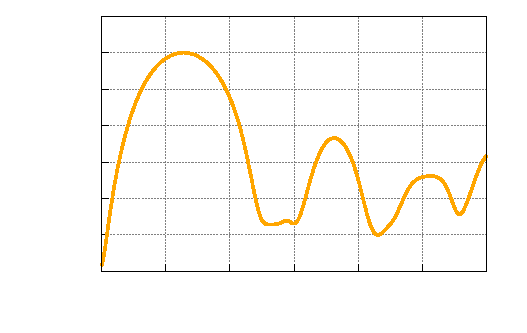
\includegraphics{4P-p12-pos}}%
    \gplfronttext
  \end{picture}%
\endgroup

		\vspace{0.2\baselineskip}
		\caption{Distance between K and He$_N$ centers of mass as a function of time\label{fig:4P-p12-n-pos}}
	\end{minipage}
\hfill
	\begin{minipage}[c]{0.48\linewidth}
		\fbox{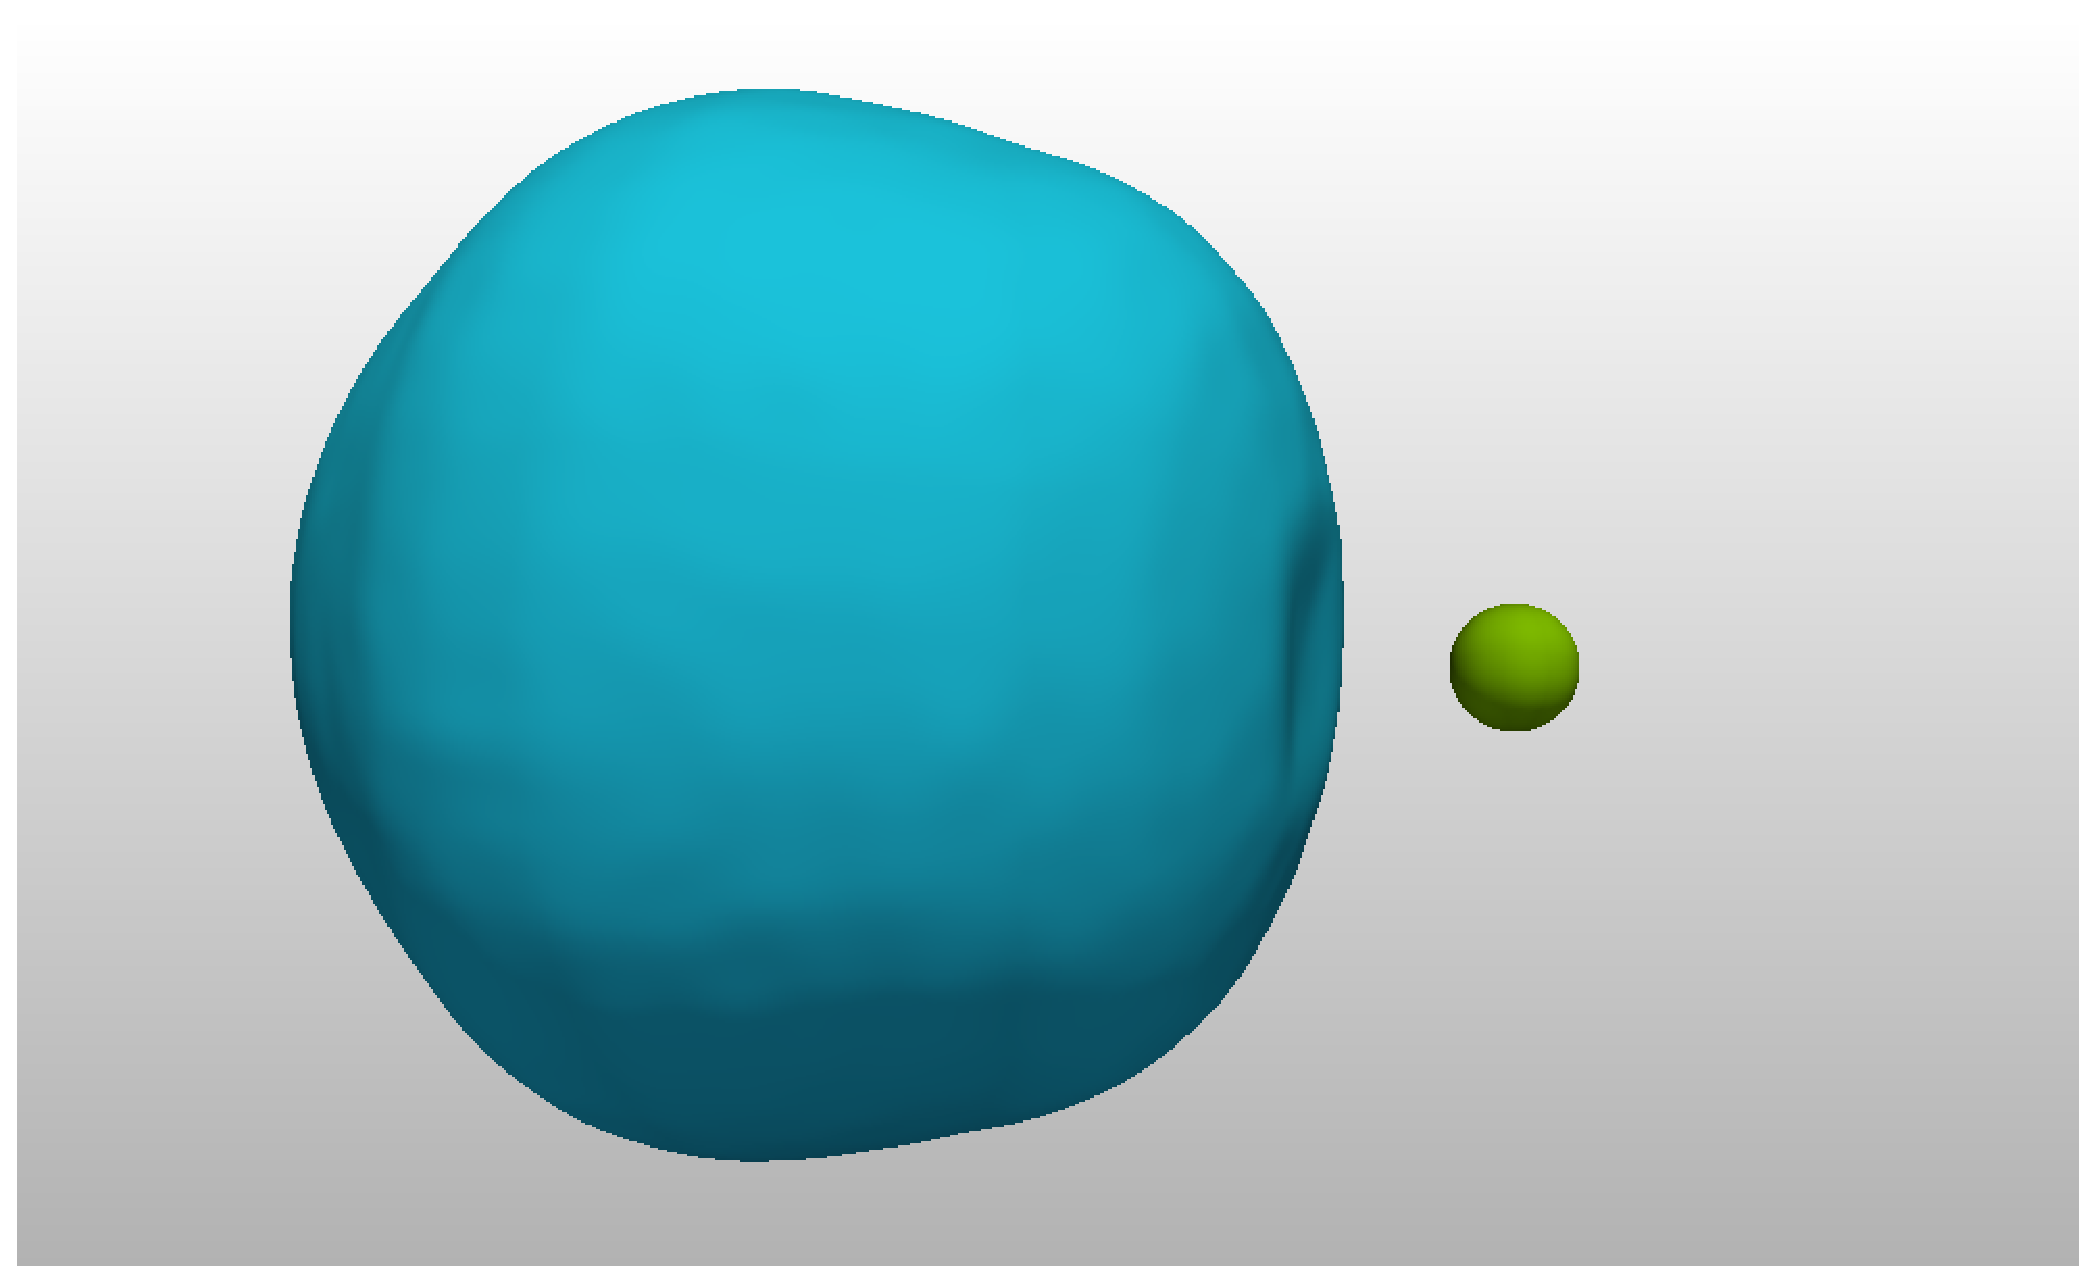
\includegraphics[scale=0.234]{4P-p12-n-snap}}
		\caption{Snapshot of He$_N$ density and bouncing K at $t=182$ ps \label{fig:4P-p12-n-snap}}
	\end{minipage}
\end{figure}

\begin{figure}[h!]
\centering
	\begin{minipage}[c]{0.48\linewidth}
		% GNUPLOT: LaTeX picture with Postscript
\begingroup
  \makeatletter
  \providecommand\color[2][]{%
    \GenericError{(gnuplot) \space\space\space\@spaces}{%
      Package color not loaded in conjunction with
      terminal option `colourtext'%
    }{See the gnuplot documentation for explanation.%
    }{Either use 'blacktext' in gnuplot or load the package
      color.sty in LaTeX.}%
    \renewcommand\color[2][]{}%
  }%
  \providecommand\includegraphics[2][]{%
    \GenericError{(gnuplot) \space\space\space\@spaces}{%
      Package graphicx or graphics not loaded%
    }{See the gnuplot documentation for explanation.%
    }{The gnuplot epslatex terminal needs graphicx.sty or graphics.sty.}%
    \renewcommand\includegraphics[2][]{}%
  }%
  \providecommand\rotatebox[2]{#2}%
  \@ifundefined{ifGPcolor}{%
    \newif\ifGPcolor
    \GPcolortrue
  }{}%
  \@ifundefined{ifGPblacktext}{%
    \newif\ifGPblacktext
    \GPblacktextfalse
  }{}%
  % define a \g@addto@macro without @ in the name:
  \let\gplgaddtomacro\g@addto@macro
  % define empty templates for all commands taking text:
  \gdef\gplbacktext{}%
  \gdef\gplfronttext{}%
  \makeatother
  \ifGPblacktext
    % no textcolor at all
    \def\colorrgb#1{}%
    \def\colorgray#1{}%
  \else
    % gray or color?
    \ifGPcolor
      \def\colorrgb#1{\color[rgb]{#1}}%
      \def\colorgray#1{\color[gray]{#1}}%
      \expandafter\def\csname LTw\endcsname{\color{white}}%
      \expandafter\def\csname LTb\endcsname{\color{black}}%
      \expandafter\def\csname LTa\endcsname{\color{black}}%
      \expandafter\def\csname LT0\endcsname{\color[rgb]{1,0,0}}%
      \expandafter\def\csname LT1\endcsname{\color[rgb]{0,1,0}}%
      \expandafter\def\csname LT2\endcsname{\color[rgb]{0,0,1}}%
      \expandafter\def\csname LT3\endcsname{\color[rgb]{1,0,1}}%
      \expandafter\def\csname LT4\endcsname{\color[rgb]{0,1,1}}%
      \expandafter\def\csname LT5\endcsname{\color[rgb]{1,1,0}}%
      \expandafter\def\csname LT6\endcsname{\color[rgb]{0,0,0}}%
      \expandafter\def\csname LT7\endcsname{\color[rgb]{1,0.3,0}}%
      \expandafter\def\csname LT8\endcsname{\color[rgb]{0.5,0.5,0.5}}%
    \else
      % gray
      \def\colorrgb#1{\color{black}}%
      \def\colorgray#1{\color[gray]{#1}}%
      \expandafter\def\csname LTw\endcsname{\color{white}}%
      \expandafter\def\csname LTb\endcsname{\color{black}}%
      \expandafter\def\csname LTa\endcsname{\color{black}}%
      \expandafter\def\csname LT0\endcsname{\color{black}}%
      \expandafter\def\csname LT1\endcsname{\color{black}}%
      \expandafter\def\csname LT2\endcsname{\color{black}}%
      \expandafter\def\csname LT3\endcsname{\color{black}}%
      \expandafter\def\csname LT4\endcsname{\color{black}}%
      \expandafter\def\csname LT5\endcsname{\color{black}}%
      \expandafter\def\csname LT6\endcsname{\color{black}}%
      \expandafter\def\csname LT7\endcsname{\color{black}}%
      \expandafter\def\csname LT8\endcsname{\color{black}}%
    \fi
  \fi
    \setlength{\unitlength}{0.0500bp}%
    \ifx\gptboxheight\undefined%
      \newlength{\gptboxheight}%
      \newlength{\gptboxwidth}%
      \newsavebox{\gptboxtext}%
    \fi%
    \setlength{\fboxrule}{0.5pt}%
    \setlength{\fboxsep}{1pt}%
\begin{picture}(4752.00,2880.00)%
    \gplgaddtomacro\gplbacktext{%
      \csname LTb\endcsname%
      \put(708,432){\makebox(0,0)[r]{\strut{}$0$}}%
      \csname LTb\endcsname%
      \put(708,921){\makebox(0,0)[r]{\strut{}$0.2$}}%
      \csname LTb\endcsname%
      \put(708,1411){\makebox(0,0)[r]{\strut{}$0.4$}}%
      \csname LTb\endcsname%
      \put(708,1900){\makebox(0,0)[r]{\strut{}$0.6$}}%
      \csname LTb\endcsname%
      \put(708,2390){\makebox(0,0)[r]{\strut{}$0.8$}}%
      \csname LTb\endcsname%
      \put(708,2879){\makebox(0,0)[r]{\strut{}$1$}}%
      \csname LTb\endcsname%
      \put(840,212){\makebox(0,0){\strut{}$0$}}%
      \csname LTb\endcsname%
      \put(1452,212){\makebox(0,0){\strut{}$40$}}%
      \csname LTb\endcsname%
      \put(2064,212){\makebox(0,0){\strut{}$80$}}%
      \csname LTb\endcsname%
      \put(2677,212){\makebox(0,0){\strut{}$120$}}%
      \csname LTb\endcsname%
      \put(3289,212){\makebox(0,0){\strut{}$160$}}%
      \csname LTb\endcsname%
      \put(3901,212){\makebox(0,0){\strut{}$200$}}%
      \csname LTb\endcsname%
      \put(4513,212){\makebox(0,0){\strut{}$240$}}%
    }%
    \gplgaddtomacro\gplfronttext{%
      \csname LTb\endcsname%
      \put(176,1655){\rotatebox{-270}{\makebox(0,0){\strut{}$|\langle p, s|\lambda\rangle|^2$}}}%
      \put(2676,-74){\makebox(0,0){\strut{}Time (ps)}}%
      \csname LTb\endcsname%
      \put(2837,1766){\makebox(0,0)[r]{\strut{}$\langle p_{1},- |$}}%
      \csname LTb\endcsname%
      \put(2837,1546){\makebox(0,0)[r]{\strut{}$\langle p_{0},+ |$}}%
    }%
    \gplbacktext
    \put(0,0){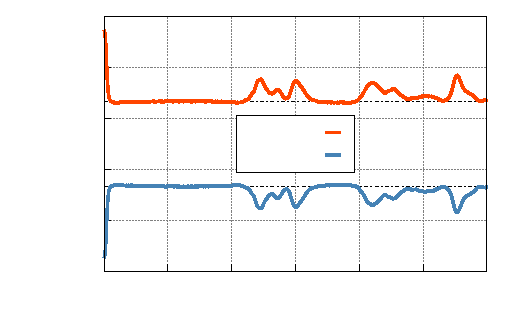
\includegraphics{4P-p12-n-proj}}%
    \gplfronttext
  \end{picture}%
\endgroup

		\vspace{0.2\baselineskip}
		\caption{Evolution of the electronic state as a function of time\label{fig:4P-p12-n-proj}}
	\end{minipage}
\hfill
	\begin{minipage}[c]{0.48\linewidth}
		% GNUPLOT: LaTeX picture with Postscript
\begingroup
  \makeatletter
  \providecommand\color[2][]{%
    \GenericError{(gnuplot) \space\space\space\@spaces}{%
      Package color not loaded in conjunction with
      terminal option `colourtext'%
    }{See the gnuplot documentation for explanation.%
    }{Either use 'blacktext' in gnuplot or load the package
      color.sty in LaTeX.}%
    \renewcommand\color[2][]{}%
  }%
  \providecommand\includegraphics[2][]{%
    \GenericError{(gnuplot) \space\space\space\@spaces}{%
      Package graphicx or graphics not loaded%
    }{See the gnuplot documentation for explanation.%
    }{The gnuplot epslatex terminal needs graphicx.sty or graphics.sty.}%
    \renewcommand\includegraphics[2][]{}%
  }%
  \providecommand\rotatebox[2]{#2}%
  \@ifundefined{ifGPcolor}{%
    \newif\ifGPcolor
    \GPcolortrue
  }{}%
  \@ifundefined{ifGPblacktext}{%
    \newif\ifGPblacktext
    \GPblacktextfalse
  }{}%
  % define a \g@addto@macro without @ in the name:
  \let\gplgaddtomacro\g@addto@macro
  % define empty templates for all commands taking text:
  \gdef\gplbacktext{}%
  \gdef\gplfronttext{}%
  \makeatother
  \ifGPblacktext
    % no textcolor at all
    \def\colorrgb#1{}%
    \def\colorgray#1{}%
  \else
    % gray or color?
    \ifGPcolor
      \def\colorrgb#1{\color[rgb]{#1}}%
      \def\colorgray#1{\color[gray]{#1}}%
      \expandafter\def\csname LTw\endcsname{\color{white}}%
      \expandafter\def\csname LTb\endcsname{\color{black}}%
      \expandafter\def\csname LTa\endcsname{\color{black}}%
      \expandafter\def\csname LT0\endcsname{\color[rgb]{1,0,0}}%
      \expandafter\def\csname LT1\endcsname{\color[rgb]{0,1,0}}%
      \expandafter\def\csname LT2\endcsname{\color[rgb]{0,0,1}}%
      \expandafter\def\csname LT3\endcsname{\color[rgb]{1,0,1}}%
      \expandafter\def\csname LT4\endcsname{\color[rgb]{0,1,1}}%
      \expandafter\def\csname LT5\endcsname{\color[rgb]{1,1,0}}%
      \expandafter\def\csname LT6\endcsname{\color[rgb]{0,0,0}}%
      \expandafter\def\csname LT7\endcsname{\color[rgb]{1,0.3,0}}%
      \expandafter\def\csname LT8\endcsname{\color[rgb]{0.5,0.5,0.5}}%
    \else
      % gray
      \def\colorrgb#1{\color{black}}%
      \def\colorgray#1{\color[gray]{#1}}%
      \expandafter\def\csname LTw\endcsname{\color{white}}%
      \expandafter\def\csname LTb\endcsname{\color{black}}%
      \expandafter\def\csname LTa\endcsname{\color{black}}%
      \expandafter\def\csname LT0\endcsname{\color{black}}%
      \expandafter\def\csname LT1\endcsname{\color{black}}%
      \expandafter\def\csname LT2\endcsname{\color{black}}%
      \expandafter\def\csname LT3\endcsname{\color{black}}%
      \expandafter\def\csname LT4\endcsname{\color{black}}%
      \expandafter\def\csname LT5\endcsname{\color{black}}%
      \expandafter\def\csname LT6\endcsname{\color{black}}%
      \expandafter\def\csname LT7\endcsname{\color{black}}%
      \expandafter\def\csname LT8\endcsname{\color{black}}%
    \fi
  \fi
    \setlength{\unitlength}{0.0500bp}%
    \ifx\gptboxheight\undefined%
      \newlength{\gptboxheight}%
      \newlength{\gptboxwidth}%
      \newsavebox{\gptboxtext}%
    \fi%
    \setlength{\fboxrule}{0.5pt}%
    \setlength{\fboxsep}{1pt}%
\begin{picture}(4752.00,2880.00)%
    \gplgaddtomacro\gplbacktext{%
      \csname LTb\endcsname%
      \put(814,432){\makebox(0,0)[r]{\strut{}$-60$}}%
      \csname LTb\endcsname%
      \put(814,782){\makebox(0,0)[r]{\strut{}$-55$}}%
      \csname LTb\endcsname%
      \put(814,1131){\makebox(0,0)[r]{\strut{}$-50$}}%
      \csname LTb\endcsname%
      \put(814,1481){\makebox(0,0)[r]{\strut{}$-45$}}%
      \csname LTb\endcsname%
      \put(814,1830){\makebox(0,0)[r]{\strut{}$-40$}}%
      \csname LTb\endcsname%
      \put(814,2180){\makebox(0,0)[r]{\strut{}$-35$}}%
      \csname LTb\endcsname%
      \put(814,2529){\makebox(0,0)[r]{\strut{}$-30$}}%
      \csname LTb\endcsname%
      \put(814,2879){\makebox(0,0)[r]{\strut{}$-25$}}%
      \csname LTb\endcsname%
      \put(946,212){\makebox(0,0){\strut{}$0$}}%
      \csname LTb\endcsname%
      \put(1541,212){\makebox(0,0){\strut{}$1$}}%
      \csname LTb\endcsname%
      \put(2135,212){\makebox(0,0){\strut{}$2$}}%
      \csname LTb\endcsname%
      \put(2730,212){\makebox(0,0){\strut{}$3$}}%
      \csname LTb\endcsname%
      \put(3324,212){\makebox(0,0){\strut{}$4$}}%
      \csname LTb\endcsname%
      \put(3919,212){\makebox(0,0){\strut{}$5$}}%
      \csname LTb\endcsname%
      \put(4513,212){\makebox(0,0){\strut{}$6$}}%
    }%
    \gplgaddtomacro\gplfronttext{%
      \csname LTb\endcsname%
      \put(176,1655){\rotatebox{-270}{\makebox(0,0){\strut{}Impurity energy (K)}}}%
      \put(2729,-74){\makebox(0,0){\strut{}Time (ps)}}%
    }%
    \gplbacktext
    \put(0,0){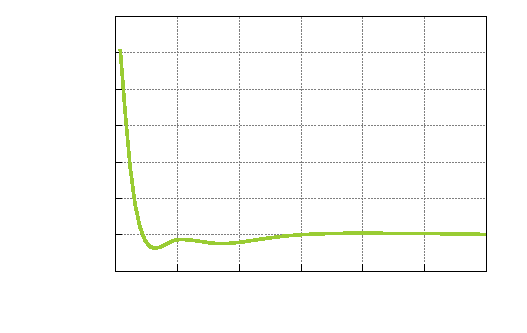
\includegraphics{4P-p12-energy}}%
    \gplfronttext
  \end{picture}%
\endgroup

		\vspace{0.2\baselineskip}
		\caption{Total potassium energy as a function of time\label{fig:4P-p12-n-energy}}
	\end{minipage}
\end{figure}
	
After excitation to the $\Pi_{1/2}$ state the potassium does not leave the droplet as can be seen in \citfig{fig:4P-p12-n-pos}.
Moreover the 3D snapshot \citfig{fig:4P-p12-n-snap} shows no exciplex formation. 
This behavior can look surprising at first  because  the pair potential is repulsive and the averaged potential shows that K has enough potential energy at $t=0$ to dissociate (cf \citfig{fig:DIM-4p-pot}). 
One can actually easily understand what is going on by plotting the total impurity energy as a function of time.
As shown in \citfig{fig:4P-p12-n-energy}, K is giving a lot of energy to the droplet: up to 25 K. 
On the other hand the $\Pi_{1/2}$ pair potential has a tiny well about +4.0 \AA{} away from the initial position, which creates both a long range attraction and a barrier when the particle is coming back. 
These two phenomena explain why we have a bouncing-bound K.
In particular we see that the bouncing occurs at around +2.5 \AA{}, which is consistent with the previous explanation. 
One can also understand why there is no exciplex formation: the deep well in the pair potential is not accessible due to the tiny barrier.\\

The electronic state evolution for $\Pi_{1/2}$ excitation is presented in \citfig{fig:4P-p12-n-proj}.
The situation is similar to that of $\Sigma_{1/2}$ excitation because $\Omega=1/2$, but here $\Lambda \approx 1$ and $J\approx 1/2$ so that $\ket{p_1,-}$ is dominant at small distance and we find $\ket{J=1/2,\Omega=1/2}$ at large distances.
In particular we note that when K is bouncing we are in an intermediate case.

\subsubsection{Displacing the excitation position}

The previous discussion showed that the tiny barrier close to the excitation region plays an important role. 
It is therefore interesting to see what happens when the initial position of K is slightly shifted.
This could occur either due to thermal excitation or to quantum delocalization.
One can use diabatic potentials and ground state K wave function (see \citfig{fig:4S-potentials}) to determine the order of magnitude of a reasonable shift.
It appears that both thermal (0.4~K) and quantum (half of the maximum of the wave function) fluctuations give a possible $\pm$0.5 \AA{} shift for the excitation position.
%
\begin{figure}[h!]
\centering
	\begin{minipage}[c]{0.48\linewidth}
		% GNUPLOT: LaTeX picture with Postscript
\begingroup
  \makeatletter
  \providecommand\color[2][]{%
    \GenericError{(gnuplot) \space\space\space\@spaces}{%
      Package color not loaded in conjunction with
      terminal option `colourtext'%
    }{See the gnuplot documentation for explanation.%
    }{Either use 'blacktext' in gnuplot or load the package
      color.sty in LaTeX.}%
    \renewcommand\color[2][]{}%
  }%
  \providecommand\includegraphics[2][]{%
    \GenericError{(gnuplot) \space\space\space\@spaces}{%
      Package graphicx or graphics not loaded%
    }{See the gnuplot documentation for explanation.%
    }{The gnuplot epslatex terminal needs graphicx.sty or graphics.sty.}%
    \renewcommand\includegraphics[2][]{}%
  }%
  \providecommand\rotatebox[2]{#2}%
  \@ifundefined{ifGPcolor}{%
    \newif\ifGPcolor
    \GPcolortrue
  }{}%
  \@ifundefined{ifGPblacktext}{%
    \newif\ifGPblacktext
    \GPblacktextfalse
  }{}%
  % define a \g@addto@macro without @ in the name:
  \let\gplgaddtomacro\g@addto@macro
  % define empty templates for all commands taking text:
  \gdef\gplbacktext{}%
  \gdef\gplfronttext{}%
  \makeatother
  \ifGPblacktext
    % no textcolor at all
    \def\colorrgb#1{}%
    \def\colorgray#1{}%
  \else
    % gray or color?
    \ifGPcolor
      \def\colorrgb#1{\color[rgb]{#1}}%
      \def\colorgray#1{\color[gray]{#1}}%
      \expandafter\def\csname LTw\endcsname{\color{white}}%
      \expandafter\def\csname LTb\endcsname{\color{black}}%
      \expandafter\def\csname LTa\endcsname{\color{black}}%
      \expandafter\def\csname LT0\endcsname{\color[rgb]{1,0,0}}%
      \expandafter\def\csname LT1\endcsname{\color[rgb]{0,1,0}}%
      \expandafter\def\csname LT2\endcsname{\color[rgb]{0,0,1}}%
      \expandafter\def\csname LT3\endcsname{\color[rgb]{1,0,1}}%
      \expandafter\def\csname LT4\endcsname{\color[rgb]{0,1,1}}%
      \expandafter\def\csname LT5\endcsname{\color[rgb]{1,1,0}}%
      \expandafter\def\csname LT6\endcsname{\color[rgb]{0,0,0}}%
      \expandafter\def\csname LT7\endcsname{\color[rgb]{1,0.3,0}}%
      \expandafter\def\csname LT8\endcsname{\color[rgb]{0.5,0.5,0.5}}%
    \else
      % gray
      \def\colorrgb#1{\color{black}}%
      \def\colorgray#1{\color[gray]{#1}}%
      \expandafter\def\csname LTw\endcsname{\color{white}}%
      \expandafter\def\csname LTb\endcsname{\color{black}}%
      \expandafter\def\csname LTa\endcsname{\color{black}}%
      \expandafter\def\csname LT0\endcsname{\color{black}}%
      \expandafter\def\csname LT1\endcsname{\color{black}}%
      \expandafter\def\csname LT2\endcsname{\color{black}}%
      \expandafter\def\csname LT3\endcsname{\color{black}}%
      \expandafter\def\csname LT4\endcsname{\color{black}}%
      \expandafter\def\csname LT5\endcsname{\color{black}}%
      \expandafter\def\csname LT6\endcsname{\color{black}}%
      \expandafter\def\csname LT7\endcsname{\color{black}}%
      \expandafter\def\csname LT8\endcsname{\color{black}}%
    \fi
  \fi
    \setlength{\unitlength}{0.0500bp}%
    \ifx\gptboxheight\undefined%
      \newlength{\gptboxheight}%
      \newlength{\gptboxwidth}%
      \newsavebox{\gptboxtext}%
    \fi%
    \setlength{\fboxrule}{0.5pt}%
    \setlength{\fboxsep}{1pt}%
\begin{picture}(4752.00,2880.00)%
    \gplgaddtomacro\gplbacktext{%
      \csname LTb\endcsname%
      \put(814,432){\makebox(0,0)[r]{\strut{}$0$}}%
      \csname LTb\endcsname%
      \put(814,921){\makebox(0,0)[r]{\strut{}$0.2$}}%
      \csname LTb\endcsname%
      \put(814,1411){\makebox(0,0)[r]{\strut{}$0.4$}}%
      \csname LTb\endcsname%
      \put(814,1900){\makebox(0,0)[r]{\strut{}$0.6$}}%
      \csname LTb\endcsname%
      \put(814,2390){\makebox(0,0)[r]{\strut{}$0.8$}}%
      \csname LTb\endcsname%
      \put(814,2879){\makebox(0,0)[r]{\strut{}$1$}}%
      \csname LTb\endcsname%
      \put(946,212){\makebox(0,0){\strut{}$0$}}%
      \csname LTb\endcsname%
      \put(1838,212){\makebox(0,0){\strut{}$4$}}%
      \csname LTb\endcsname%
      \put(2730,212){\makebox(0,0){\strut{}$8$}}%
      \csname LTb\endcsname%
      \put(3621,212){\makebox(0,0){\strut{}$12$}}%
      \csname LTb\endcsname%
      \put(4513,212){\makebox(0,0){\strut{}$16$}}%
    }%
    \gplgaddtomacro\gplfronttext{%
      \csname LTb\endcsname%
      \put(176,1655){\rotatebox{-270}{\makebox(0,0){\strut{}Intensity (arb. unit)}}}%
      \put(2729,-74){\makebox(0,0){\strut{}Energy (cm$^{-1}$)}}%
      \csname LTb\endcsname%
      \put(2209,2096){\makebox(0,0)[r]{\strut{}$\langle p_{+1},-|$}}%
      \csname LTb\endcsname%
      \put(2209,1876){\makebox(0,0)[r]{\strut{}$\langle p_{-1},-|$}}%
      \csname LTb\endcsname%
      \put(2209,1656){\makebox(0,0)[r]{\strut{}$\langle p_{0},+|$}}%
      \csname LTb\endcsname%
      \put(2209,1436){\makebox(0,0)[r]{\strut{}$\langle p_{x},-|$}}%
      \csname LTb\endcsname%
      \put(2209,1216){\makebox(0,0)[r]{\strut{}$\langle p_{y},-|$}}%
    }%
    \gplbacktext
    \put(0,0){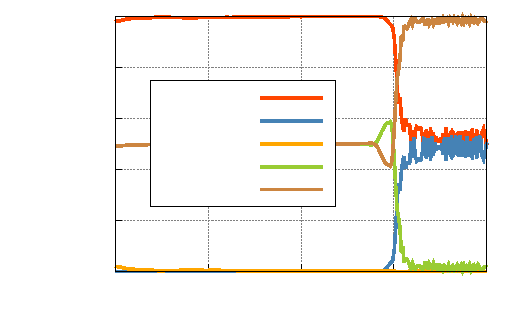
\includegraphics{4P-p12-d-proj}}%
    \gplfronttext
  \end{picture}%
\endgroup

		\vspace{0.2\baselineskip}
		\caption{Evolution of the electronic state as a function of time\label{fig:4P-p12-d-proj}}
	\end{minipage}
\hfill
	\begin{minipage}[c]{0.48\linewidth}
		% GNUPLOT: LaTeX picture with Postscript
\begingroup
  \makeatletter
  \providecommand\color[2][]{%
    \GenericError{(gnuplot) \space\space\space\@spaces}{%
      Package color not loaded in conjunction with
      terminal option `colourtext'%
    }{See the gnuplot documentation for explanation.%
    }{Either use 'blacktext' in gnuplot or load the package
      color.sty in LaTeX.}%
    \renewcommand\color[2][]{}%
  }%
  \providecommand\includegraphics[2][]{%
    \GenericError{(gnuplot) \space\space\space\@spaces}{%
      Package graphicx or graphics not loaded%
    }{See the gnuplot documentation for explanation.%
    }{The gnuplot epslatex terminal needs graphicx.sty or graphics.sty.}%
    \renewcommand\includegraphics[2][]{}%
  }%
  \providecommand\rotatebox[2]{#2}%
  \@ifundefined{ifGPcolor}{%
    \newif\ifGPcolor
    \GPcolortrue
  }{}%
  \@ifundefined{ifGPblacktext}{%
    \newif\ifGPblacktext
    \GPblacktextfalse
  }{}%
  % define a \g@addto@macro without @ in the name:
  \let\gplgaddtomacro\g@addto@macro
  % define empty templates for all commands taking text:
  \gdef\gplbacktext{}%
  \gdef\gplfronttext{}%
  \makeatother
  \ifGPblacktext
    % no textcolor at all
    \def\colorrgb#1{}%
    \def\colorgray#1{}%
  \else
    % gray or color?
    \ifGPcolor
      \def\colorrgb#1{\color[rgb]{#1}}%
      \def\colorgray#1{\color[gray]{#1}}%
      \expandafter\def\csname LTw\endcsname{\color{white}}%
      \expandafter\def\csname LTb\endcsname{\color{black}}%
      \expandafter\def\csname LTa\endcsname{\color{black}}%
      \expandafter\def\csname LT0\endcsname{\color[rgb]{1,0,0}}%
      \expandafter\def\csname LT1\endcsname{\color[rgb]{0,1,0}}%
      \expandafter\def\csname LT2\endcsname{\color[rgb]{0,0,1}}%
      \expandafter\def\csname LT3\endcsname{\color[rgb]{1,0,1}}%
      \expandafter\def\csname LT4\endcsname{\color[rgb]{0,1,1}}%
      \expandafter\def\csname LT5\endcsname{\color[rgb]{1,1,0}}%
      \expandafter\def\csname LT6\endcsname{\color[rgb]{0,0,0}}%
      \expandafter\def\csname LT7\endcsname{\color[rgb]{1,0.3,0}}%
      \expandafter\def\csname LT8\endcsname{\color[rgb]{0.5,0.5,0.5}}%
    \else
      % gray
      \def\colorrgb#1{\color{black}}%
      \def\colorgray#1{\color[gray]{#1}}%
      \expandafter\def\csname LTw\endcsname{\color{white}}%
      \expandafter\def\csname LTb\endcsname{\color{black}}%
      \expandafter\def\csname LTa\endcsname{\color{black}}%
      \expandafter\def\csname LT0\endcsname{\color{black}}%
      \expandafter\def\csname LT1\endcsname{\color{black}}%
      \expandafter\def\csname LT2\endcsname{\color{black}}%
      \expandafter\def\csname LT3\endcsname{\color{black}}%
      \expandafter\def\csname LT4\endcsname{\color{black}}%
      \expandafter\def\csname LT5\endcsname{\color{black}}%
      \expandafter\def\csname LT6\endcsname{\color{black}}%
      \expandafter\def\csname LT7\endcsname{\color{black}}%
      \expandafter\def\csname LT8\endcsname{\color{black}}%
    \fi
  \fi
    \setlength{\unitlength}{0.0500bp}%
    \ifx\gptboxheight\undefined%
      \newlength{\gptboxheight}%
      \newlength{\gptboxwidth}%
      \newsavebox{\gptboxtext}%
    \fi%
    \setlength{\fboxrule}{0.5pt}%
    \setlength{\fboxsep}{1pt}%
\begin{picture}(4752.00,2880.00)%
    \gplgaddtomacro\gplbacktext{%
      \csname LTb\endcsname%
      \put(682,432){\makebox(0,0)[r]{\strut{}$25$}}%
      \csname LTb\endcsname%
      \put(682,840){\makebox(0,0)[r]{\strut{}$26$}}%
      \csname LTb\endcsname%
      \put(682,1248){\makebox(0,0)[r]{\strut{}$27$}}%
      \csname LTb\endcsname%
      \put(682,1656){\makebox(0,0)[r]{\strut{}$28$}}%
      \csname LTb\endcsname%
      \put(682,2063){\makebox(0,0)[r]{\strut{}$29$}}%
      \csname LTb\endcsname%
      \put(682,2471){\makebox(0,0)[r]{\strut{}$30$}}%
      \csname LTb\endcsname%
      \put(682,2879){\makebox(0,0)[r]{\strut{}$31$}}%
      \csname LTb\endcsname%
      \put(814,212){\makebox(0,0){\strut{}$0$}}%
      \csname LTb\endcsname%
      \put(1431,212){\makebox(0,0){\strut{}$10$}}%
      \csname LTb\endcsname%
      \put(2047,212){\makebox(0,0){\strut{}$20$}}%
      \csname LTb\endcsname%
      \put(2664,212){\makebox(0,0){\strut{}$30$}}%
      \csname LTb\endcsname%
      \put(3280,212){\makebox(0,0){\strut{}$40$}}%
      \csname LTb\endcsname%
      \put(3897,212){\makebox(0,0){\strut{}$50$}}%
      \csname LTb\endcsname%
      \put(4513,212){\makebox(0,0){\strut{}$60$}}%
    }%
    \gplgaddtomacro\gplfronttext{%
      \csname LTb\endcsname%
      \put(176,1655){\rotatebox{-270}{\makebox(0,0){\strut{}K relative position (\AA)}}}%
      \put(2663,-74){\makebox(0,0){\strut{}Time (ps)}}%
    }%
    \gplbacktext
    \put(0,0){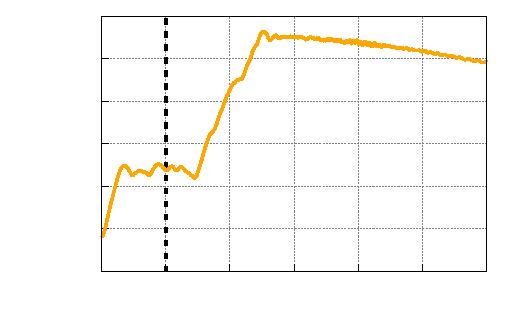
\includegraphics{4P-p12-d-pos}}%
    \gplfronttext
  \end{picture}%
\endgroup

		\vspace{0.2\baselineskip}
		\caption{Distance between K and He$_N$ centers of mass as a function of time\label{fig:4P-p12-d-pos}}
	\end{minipage}
\end{figure}

When the initial position of the potassium atom is shifted by $+$0.5 \AA{}, the dynamics is not affected.
On the opposite, when it is shifted by $-$0.5 \AA{} the situation is quite different.
At first, we observe a linear exciplex formation in 5 ps (\citfig{fig:4p-p12-d-snap-a}): helium atoms are attracted to K, and the internal state becomes a true eigenvector of $L_z$.
It it worth noting that this exciplex shape can be explained: indeed the $\ket{p_1}$ orbital has an apple shape with a tiny well at the helium position. 
One may refer to \cite{Zbi2005} to get more details about orbital shapes and their link to exciplex formation. \\

The linear exciplex lasts for 10 ps. 
After that we can clearly see a symmetry breaking: the system is violently projected into an asymmetric $\ket{p_y}$ state (\citfig{fig:4P-p12-d-proj}), and we see formation of a ring exciplexe around this orbital (\citfig{fig:4p-p12-d-snap-b}). 
This is clearly not expected, because our framework is of cylindrical symmetry and there is no physical reason to break it. 
It can be noted that this symmetry breaking happens along a well defined axis of our system. 
During the ring exciplex formation, we see  unexplained high helium density  between the droplet and the impurity in the ring plane that forces the exciplex to shift outward.  
This structure seems to disappear at long time and the exciplex is brought back closer (\citfig{fig:4P-p12-d-pos}). 
Our hypothesis is that this arises because we use a cubic grid with a step size of 0.4 \AA{} which is not small enough to describe a 1 \AA{}$^3$ exciplex in cylindrical symmetry. 
Unfortunately decreasing the  the spatial step size quickly becomes too expensive in computing time and  we cannot use a cylindrical grid (see the annex for detail).

\begin{figure}[h!]
\centering
	\begin{minipage}[c]{0.48\linewidth}
		\fbox{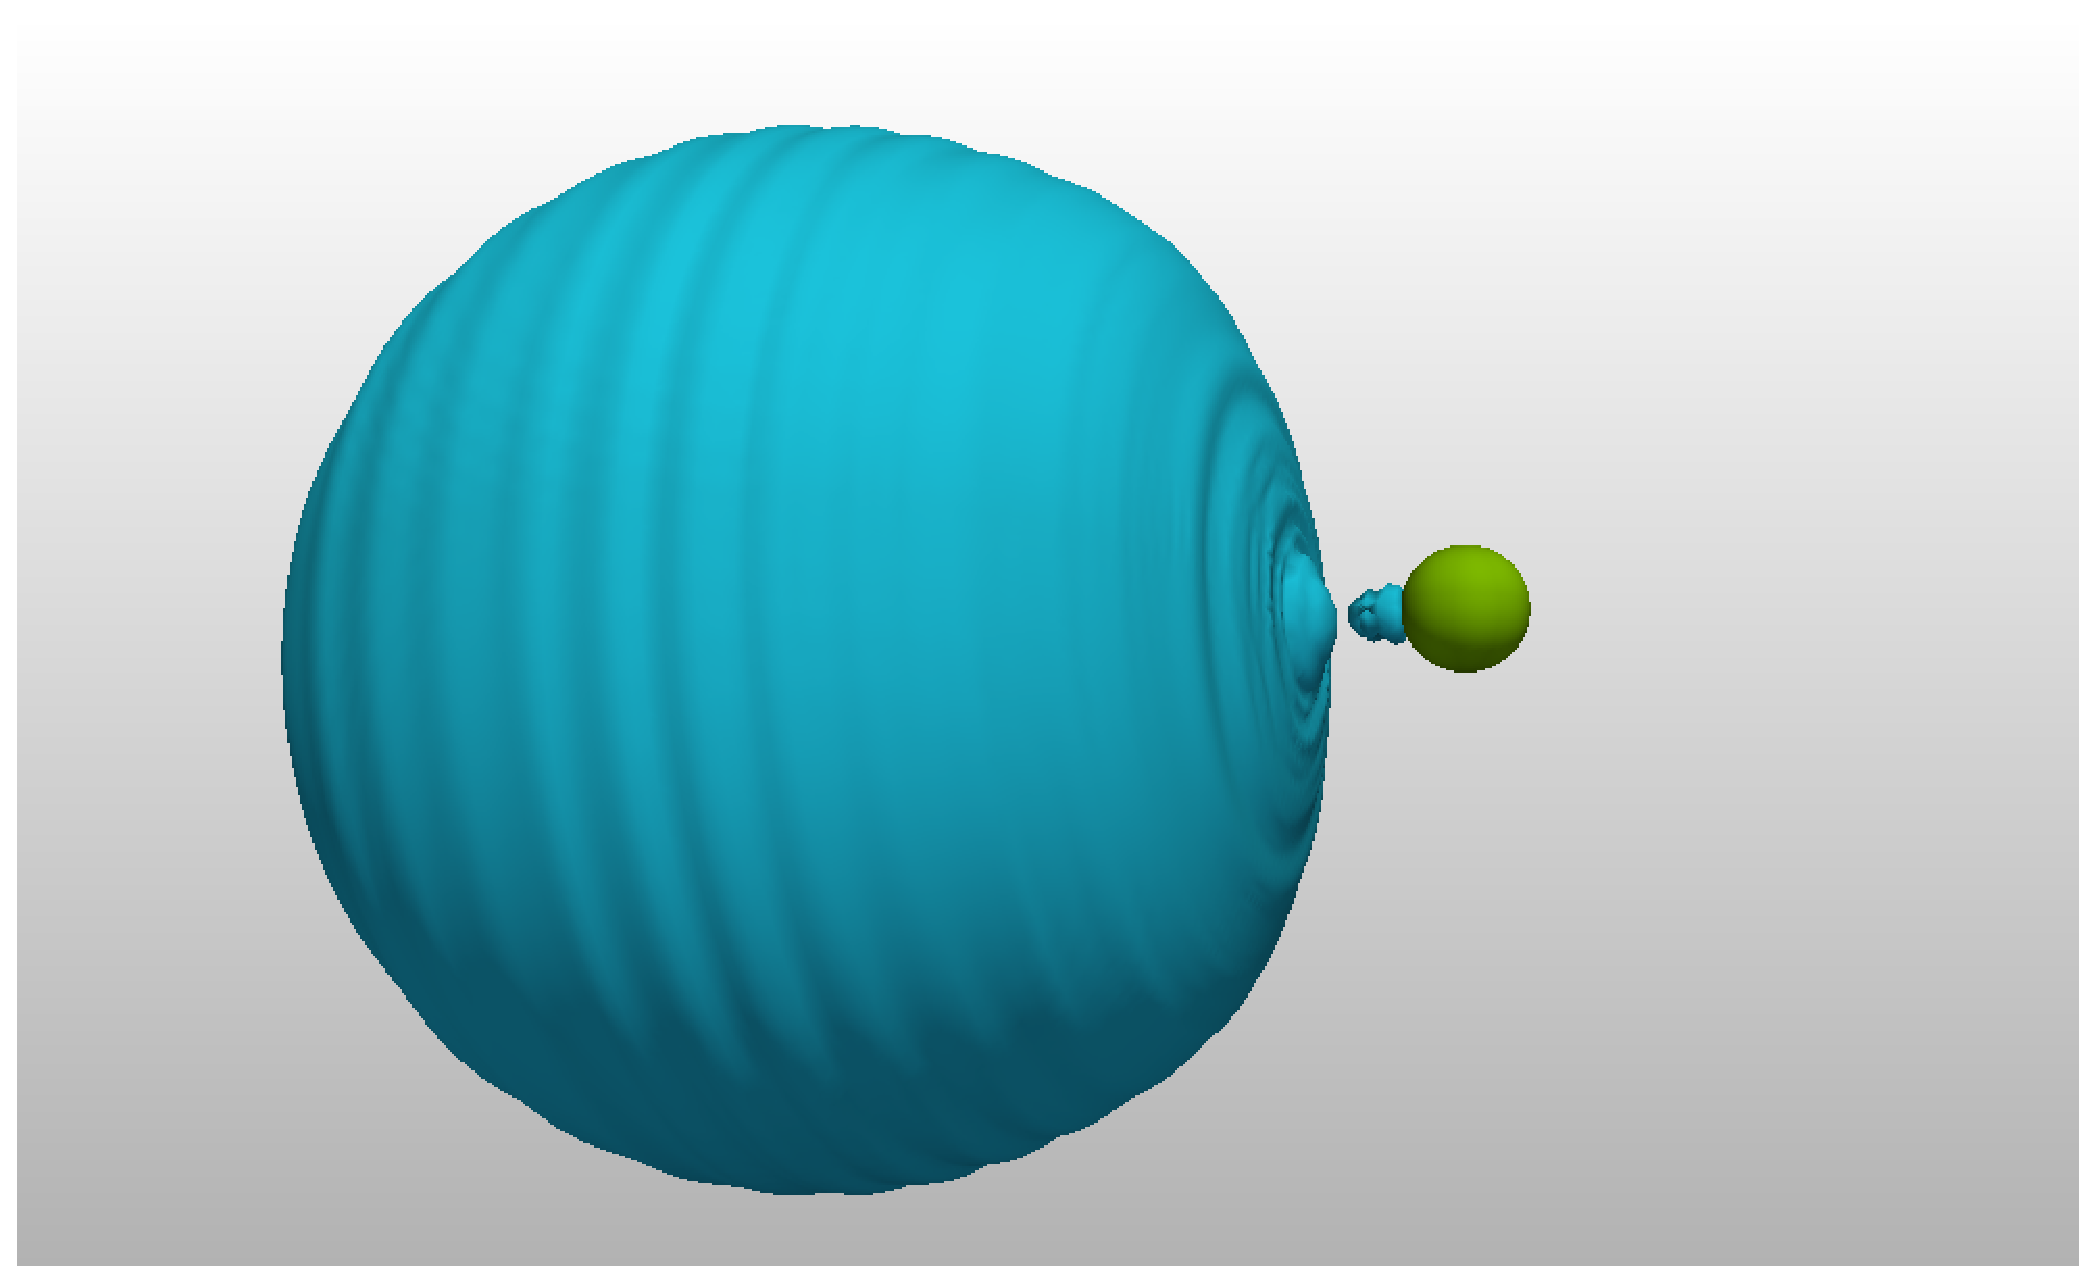
\includegraphics[scale=0.234]{4P-p12-d-snap-linear}}
		\subcaption{Linear exciplex at $t=7.5$ ps \label{fig:4p-p12-d-snap-a}}
	\end{minipage}
\hfill
	\begin{minipage}[c]{0.48\linewidth}
		\fbox{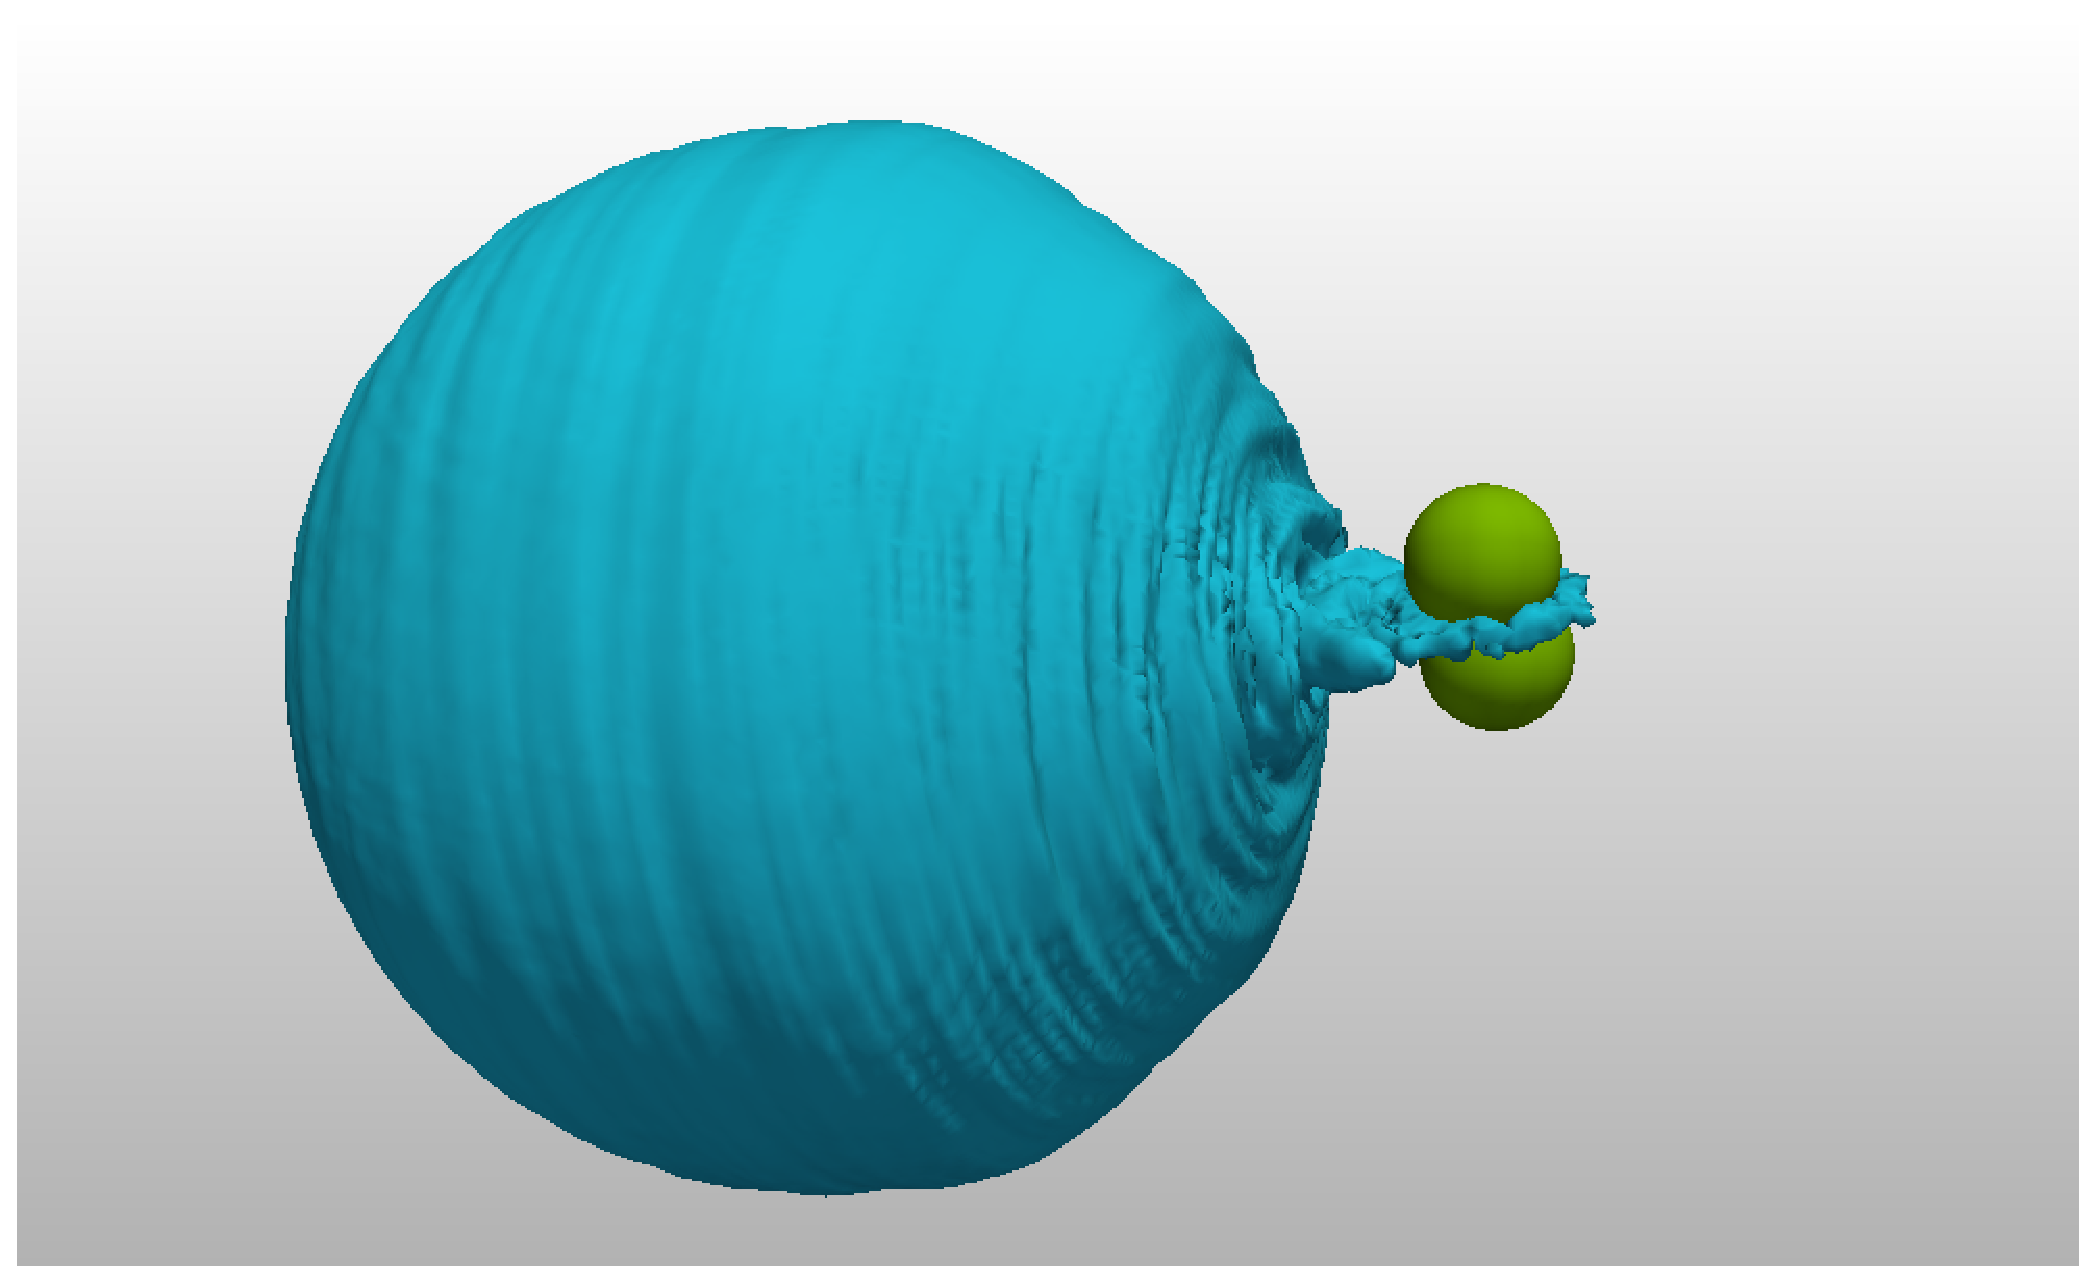
\includegraphics[scale=0.234]{4P-p12-d-snap-ring}}
		\subcaption{Ring exciplex at $t=19.5$ ps \label{fig:4p-p12-d-snap-b}}
	\end{minipage}
\vspace{-0.2\baselineskip}
\label{4P:p12-snap}
\caption{Snapshot of He$_N$ density and bound K exciplex before and after the symmetry breaking, K $p_y$ orbital is schematically represented in the second case to help the interpretation}
\end{figure}

\subsubsection{Investigations on symmetry breaking} 
\indent 
In order to test the hypothesis of the grid effect we worked with a smaller system (90 atoms) an studied the effect of grid size. 
As can be seen in \cittab{table:4P-symb}, the symmetry breaking occurs later and later as we reduce the mesh step size, which corroborates our hypothesis.
\begin{table}[h!]
\centering
\begin{tabular}{|c|c|c|c|c|}
  \hline
  Spatial step size $\delta r$ (\AA) & 0.42 & 0.28 & 0.21 & 0.14 \\
  \hline
  Appearance of the symmetry breaking (ps) & 3.2 & 5.6 & 9.0 & 10.8 \\
  \hline
\end{tabular}
\caption{Evolution of time before the occurrence of symmetry breaking  during a dynamic simulation of  $\Pi_{1/2}$ excitation for different spatial step sizes.}
\label{table:4P-symb}
\end{table}

Now we can understand what is happening: the exciplex formation creates a high density volume which is poorly described by our cubic mesh. This induces asymmetry in the density profile at the surface of the droplet near to K, which induces back an asymmetric interaction and  ends up in the projection of the internal state into an energetically more favorable configuration. 
This also explains why this projection occurs along a well defined axis of our simulation.
%
\subsection{$\Pi_{3/2}$ exciplex formation: beyond symmetry breaking investigations}

\subsubsection{Exciplex formation and symmetry breaking}

Exciting the $\Pi_{3/2}$ state leads without surprise to a linear exciplex (almost identical to \citfig{fig:4p-p12-d-snap-a}) in 4 ps, because we excite in a potential well (\citfig{fig:DIM-4p-pot}). However, in the exact same way as in the $\Pi_{1/2}$ we see that a symmetry breaking occurs. Looking at internal state projections (\citfig{fig:4P-p32-f-proj}) we see that before this symmetry breaking the internal state is actually pure in our basis, as it should, since the $\Omega=3/2$ state is  $\ket{\lambda}=\ket{p_1,+}$ (no other orbital can give $\Omega=3/2$). \\

Comparing trajectories in the $\Pi_{1/2}$  (\citfig{fig:4P-p12-d-pos}) and in the $\Pi_{3/2}$ (\citfig{fig:4P-p32-free-pos}) states shows a difference: in the $\Pi_{3/2}$ state  symmetry breaking occurs during an attempt to leave the droplet while in the $\Pi_{1/2}$ state it happens in a stationary position.

\begin{figure}[h!]
	\centering
	\begin{minipage}[c]{0.48\linewidth}
		% GNUPLOT: LaTeX picture with Postscript
\begingroup
  \makeatletter
  \providecommand\color[2][]{%
    \GenericError{(gnuplot) \space\space\space\@spaces}{%
      Package color not loaded in conjunction with
      terminal option `colourtext'%
    }{See the gnuplot documentation for explanation.%
    }{Either use 'blacktext' in gnuplot or load the package
      color.sty in LaTeX.}%
    \renewcommand\color[2][]{}%
  }%
  \providecommand\includegraphics[2][]{%
    \GenericError{(gnuplot) \space\space\space\@spaces}{%
      Package graphicx or graphics not loaded%
    }{See the gnuplot documentation for explanation.%
    }{The gnuplot epslatex terminal needs graphicx.sty or graphics.sty.}%
    \renewcommand\includegraphics[2][]{}%
  }%
  \providecommand\rotatebox[2]{#2}%
  \@ifundefined{ifGPcolor}{%
    \newif\ifGPcolor
    \GPcolortrue
  }{}%
  \@ifundefined{ifGPblacktext}{%
    \newif\ifGPblacktext
    \GPblacktextfalse
  }{}%
  % define a \g@addto@macro without @ in the name:
  \let\gplgaddtomacro\g@addto@macro
  % define empty templates for all commands taking text:
  \gdef\gplbacktext{}%
  \gdef\gplfronttext{}%
  \makeatother
  \ifGPblacktext
    % no textcolor at all
    \def\colorrgb#1{}%
    \def\colorgray#1{}%
  \else
    % gray or color?
    \ifGPcolor
      \def\colorrgb#1{\color[rgb]{#1}}%
      \def\colorgray#1{\color[gray]{#1}}%
      \expandafter\def\csname LTw\endcsname{\color{white}}%
      \expandafter\def\csname LTb\endcsname{\color{black}}%
      \expandafter\def\csname LTa\endcsname{\color{black}}%
      \expandafter\def\csname LT0\endcsname{\color[rgb]{1,0,0}}%
      \expandafter\def\csname LT1\endcsname{\color[rgb]{0,1,0}}%
      \expandafter\def\csname LT2\endcsname{\color[rgb]{0,0,1}}%
      \expandafter\def\csname LT3\endcsname{\color[rgb]{1,0,1}}%
      \expandafter\def\csname LT4\endcsname{\color[rgb]{0,1,1}}%
      \expandafter\def\csname LT5\endcsname{\color[rgb]{1,1,0}}%
      \expandafter\def\csname LT6\endcsname{\color[rgb]{0,0,0}}%
      \expandafter\def\csname LT7\endcsname{\color[rgb]{1,0.3,0}}%
      \expandafter\def\csname LT8\endcsname{\color[rgb]{0.5,0.5,0.5}}%
    \else
      % gray
      \def\colorrgb#1{\color{black}}%
      \def\colorgray#1{\color[gray]{#1}}%
      \expandafter\def\csname LTw\endcsname{\color{white}}%
      \expandafter\def\csname LTb\endcsname{\color{black}}%
      \expandafter\def\csname LTa\endcsname{\color{black}}%
      \expandafter\def\csname LT0\endcsname{\color{black}}%
      \expandafter\def\csname LT1\endcsname{\color{black}}%
      \expandafter\def\csname LT2\endcsname{\color{black}}%
      \expandafter\def\csname LT3\endcsname{\color{black}}%
      \expandafter\def\csname LT4\endcsname{\color{black}}%
      \expandafter\def\csname LT5\endcsname{\color{black}}%
      \expandafter\def\csname LT6\endcsname{\color{black}}%
      \expandafter\def\csname LT7\endcsname{\color{black}}%
      \expandafter\def\csname LT8\endcsname{\color{black}}%
    \fi
  \fi
    \setlength{\unitlength}{0.0500bp}%
    \ifx\gptboxheight\undefined%
      \newlength{\gptboxheight}%
      \newlength{\gptboxwidth}%
      \newsavebox{\gptboxtext}%
    \fi%
    \setlength{\fboxrule}{0.5pt}%
    \setlength{\fboxsep}{1pt}%
\begin{picture}(4752.00,2880.00)%
    \gplgaddtomacro\gplbacktext{%
      \csname LTb\endcsname%
      \put(708,432){\makebox(0,0)[r]{\strut{}$0$}}%
      \csname LTb\endcsname%
      \put(708,921){\makebox(0,0)[r]{\strut{}$0.2$}}%
      \csname LTb\endcsname%
      \put(708,1411){\makebox(0,0)[r]{\strut{}$0.4$}}%
      \csname LTb\endcsname%
      \put(708,1900){\makebox(0,0)[r]{\strut{}$0.6$}}%
      \csname LTb\endcsname%
      \put(708,2390){\makebox(0,0)[r]{\strut{}$0.8$}}%
      \csname LTb\endcsname%
      \put(708,2879){\makebox(0,0)[r]{\strut{}$1$}}%
      \csname LTb\endcsname%
      \put(840,212){\makebox(0,0){\strut{}$0$}}%
      \csname LTb\endcsname%
      \put(1452,212){\makebox(0,0){\strut{}$2$}}%
      \csname LTb\endcsname%
      \put(2064,212){\makebox(0,0){\strut{}$4$}}%
      \csname LTb\endcsname%
      \put(2677,212){\makebox(0,0){\strut{}$6$}}%
      \csname LTb\endcsname%
      \put(3289,212){\makebox(0,0){\strut{}$8$}}%
      \csname LTb\endcsname%
      \put(3901,212){\makebox(0,0){\strut{}$10$}}%
      \csname LTb\endcsname%
      \put(4513,212){\makebox(0,0){\strut{}$12$}}%
    }%
    \gplgaddtomacro\gplfronttext{%
      \csname LTb\endcsname%
      \put(176,1655){\rotatebox{-270}{\makebox(0,0){\strut{}Intensity (arb. unit)}}}%
      \put(2676,-74){\makebox(0,0){\strut{}Energy (cm$^{-1}$)}}%
      \csname LTb\endcsname%
      \put(1975,1986){\makebox(0,0)[r]{\strut{}$\langle p_{+1},+|$}}%
      \csname LTb\endcsname%
      \put(1975,1766){\makebox(0,0)[r]{\strut{}$\langle p_{-1},+|$}}%
      \csname LTb\endcsname%
      \put(1975,1546){\makebox(0,0)[r]{\strut{}$\langle p_{x},+|$}}%
      \csname LTb\endcsname%
      \put(1975,1326){\makebox(0,0)[r]{\strut{}$\langle p_{y},+|$}}%
    }%
    \gplbacktext
    \put(0,0){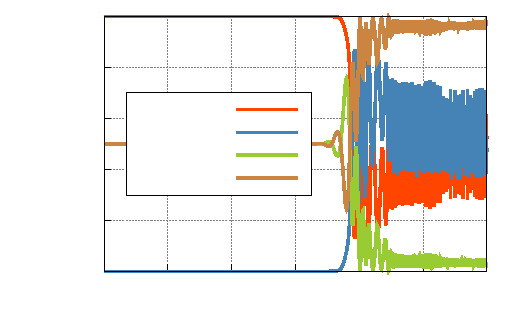
\includegraphics{4P-p32-f-proj}}%
    \gplfronttext
  \end{picture}%
\endgroup

		\vspace{0.2\baselineskip}
		\caption{Evolution of the electronic state as a function of time\label{fig:4P-p32-f-proj}}
	\end{minipage}
\hfill
	\begin{minipage}[c]{0.48\linewidth}
		% GNUPLOT: LaTeX picture with Postscript
\begingroup
  \makeatletter
  \providecommand\color[2][]{%
    \GenericError{(gnuplot) \space\space\space\@spaces}{%
      Package color not loaded in conjunction with
      terminal option `colourtext'%
    }{See the gnuplot documentation for explanation.%
    }{Either use 'blacktext' in gnuplot or load the package
      color.sty in LaTeX.}%
    \renewcommand\color[2][]{}%
  }%
  \providecommand\includegraphics[2][]{%
    \GenericError{(gnuplot) \space\space\space\@spaces}{%
      Package graphicx or graphics not loaded%
    }{See the gnuplot documentation for explanation.%
    }{The gnuplot epslatex terminal needs graphicx.sty or graphics.sty.}%
    \renewcommand\includegraphics[2][]{}%
  }%
  \providecommand\rotatebox[2]{#2}%
  \@ifundefined{ifGPcolor}{%
    \newif\ifGPcolor
    \GPcolortrue
  }{}%
  \@ifundefined{ifGPblacktext}{%
    \newif\ifGPblacktext
    \GPblacktextfalse
  }{}%
  % define a \g@addto@macro without @ in the name:
  \let\gplgaddtomacro\g@addto@macro
  % define empty templates for all commands taking text:
  \gdef\gplbacktext{}%
  \gdef\gplfronttext{}%
  \makeatother
  \ifGPblacktext
    % no textcolor at all
    \def\colorrgb#1{}%
    \def\colorgray#1{}%
  \else
    % gray or color?
    \ifGPcolor
      \def\colorrgb#1{\color[rgb]{#1}}%
      \def\colorgray#1{\color[gray]{#1}}%
      \expandafter\def\csname LTw\endcsname{\color{white}}%
      \expandafter\def\csname LTb\endcsname{\color{black}}%
      \expandafter\def\csname LTa\endcsname{\color{black}}%
      \expandafter\def\csname LT0\endcsname{\color[rgb]{1,0,0}}%
      \expandafter\def\csname LT1\endcsname{\color[rgb]{0,1,0}}%
      \expandafter\def\csname LT2\endcsname{\color[rgb]{0,0,1}}%
      \expandafter\def\csname LT3\endcsname{\color[rgb]{1,0,1}}%
      \expandafter\def\csname LT4\endcsname{\color[rgb]{0,1,1}}%
      \expandafter\def\csname LT5\endcsname{\color[rgb]{1,1,0}}%
      \expandafter\def\csname LT6\endcsname{\color[rgb]{0,0,0}}%
      \expandafter\def\csname LT7\endcsname{\color[rgb]{1,0.3,0}}%
      \expandafter\def\csname LT8\endcsname{\color[rgb]{0.5,0.5,0.5}}%
    \else
      % gray
      \def\colorrgb#1{\color{black}}%
      \def\colorgray#1{\color[gray]{#1}}%
      \expandafter\def\csname LTw\endcsname{\color{white}}%
      \expandafter\def\csname LTb\endcsname{\color{black}}%
      \expandafter\def\csname LTa\endcsname{\color{black}}%
      \expandafter\def\csname LT0\endcsname{\color{black}}%
      \expandafter\def\csname LT1\endcsname{\color{black}}%
      \expandafter\def\csname LT2\endcsname{\color{black}}%
      \expandafter\def\csname LT3\endcsname{\color{black}}%
      \expandafter\def\csname LT4\endcsname{\color{black}}%
      \expandafter\def\csname LT5\endcsname{\color{black}}%
      \expandafter\def\csname LT6\endcsname{\color{black}}%
      \expandafter\def\csname LT7\endcsname{\color{black}}%
      \expandafter\def\csname LT8\endcsname{\color{black}}%
    \fi
  \fi
    \setlength{\unitlength}{0.0500bp}%
    \ifx\gptboxheight\undefined%
      \newlength{\gptboxheight}%
      \newlength{\gptboxwidth}%
      \newsavebox{\gptboxtext}%
    \fi%
    \setlength{\fboxrule}{0.5pt}%
    \setlength{\fboxsep}{1pt}%
\begin{picture}(4752.00,2880.00)%
    \gplgaddtomacro\gplbacktext{%
      \csname LTb\endcsname%
      \put(682,432){\makebox(0,0)[r]{\strut{}$26$}}%
      \csname LTb\endcsname%
      \put(682,921){\makebox(0,0)[r]{\strut{}$27$}}%
      \csname LTb\endcsname%
      \put(682,1411){\makebox(0,0)[r]{\strut{}$28$}}%
      \csname LTb\endcsname%
      \put(682,1900){\makebox(0,0)[r]{\strut{}$29$}}%
      \csname LTb\endcsname%
      \put(682,2390){\makebox(0,0)[r]{\strut{}$30$}}%
      \csname LTb\endcsname%
      \put(682,2879){\makebox(0,0)[r]{\strut{}$31$}}%
      \csname LTb\endcsname%
      \put(814,212){\makebox(0,0){\strut{}$0$}}%
      \csname LTb\endcsname%
      \put(1554,212){\makebox(0,0){\strut{}$5$}}%
      \csname LTb\endcsname%
      \put(2294,212){\makebox(0,0){\strut{}$10$}}%
      \csname LTb\endcsname%
      \put(3033,212){\makebox(0,0){\strut{}$15$}}%
      \csname LTb\endcsname%
      \put(3773,212){\makebox(0,0){\strut{}$20$}}%
      \csname LTb\endcsname%
      \put(4513,212){\makebox(0,0){\strut{}$25$}}%
    }%
    \gplgaddtomacro\gplfronttext{%
      \csname LTb\endcsname%
      \put(176,1655){\rotatebox{-270}{\makebox(0,0){\strut{}K relative position (\AA)}}}%
      \put(2663,-74){\makebox(0,0){\strut{}Time (ps)}}%
    }%
    \gplbacktext
    \put(0,0){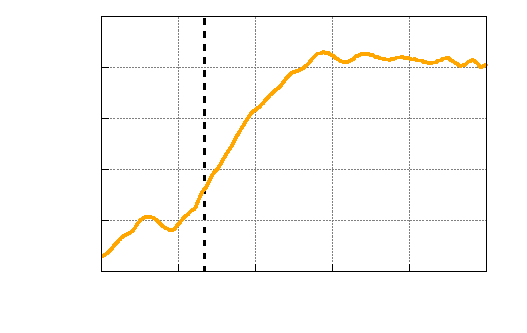
\includegraphics{4P-p32-free-pos}}%
    \gplfronttext
  \end{picture}%
\endgroup

		\vspace{0.2\baselineskip}
		\caption{Distance between K and He$_N$ centers of mass as a function of time\label{fig:4P-p32-free-pos}}
	\end{minipage}
\end{figure}

\subsubsection{Fixing internal state evolution}

We can use the fact that there is no possible evolution for the internal state\footnote{At least in our cylindrical framework} to fix it instead of let it freely evolve. 
As can be seen in \citfig{fig:4P-p32-fx-snap}, in that case the linear exciplex leaves the droplet after the symmetry breaking (\citfig{fig:4P-p32-fx-snap}).

\begin{figure}[h!]
\centering
	\begin{minipage}[c]{0.48\linewidth}
		\fbox{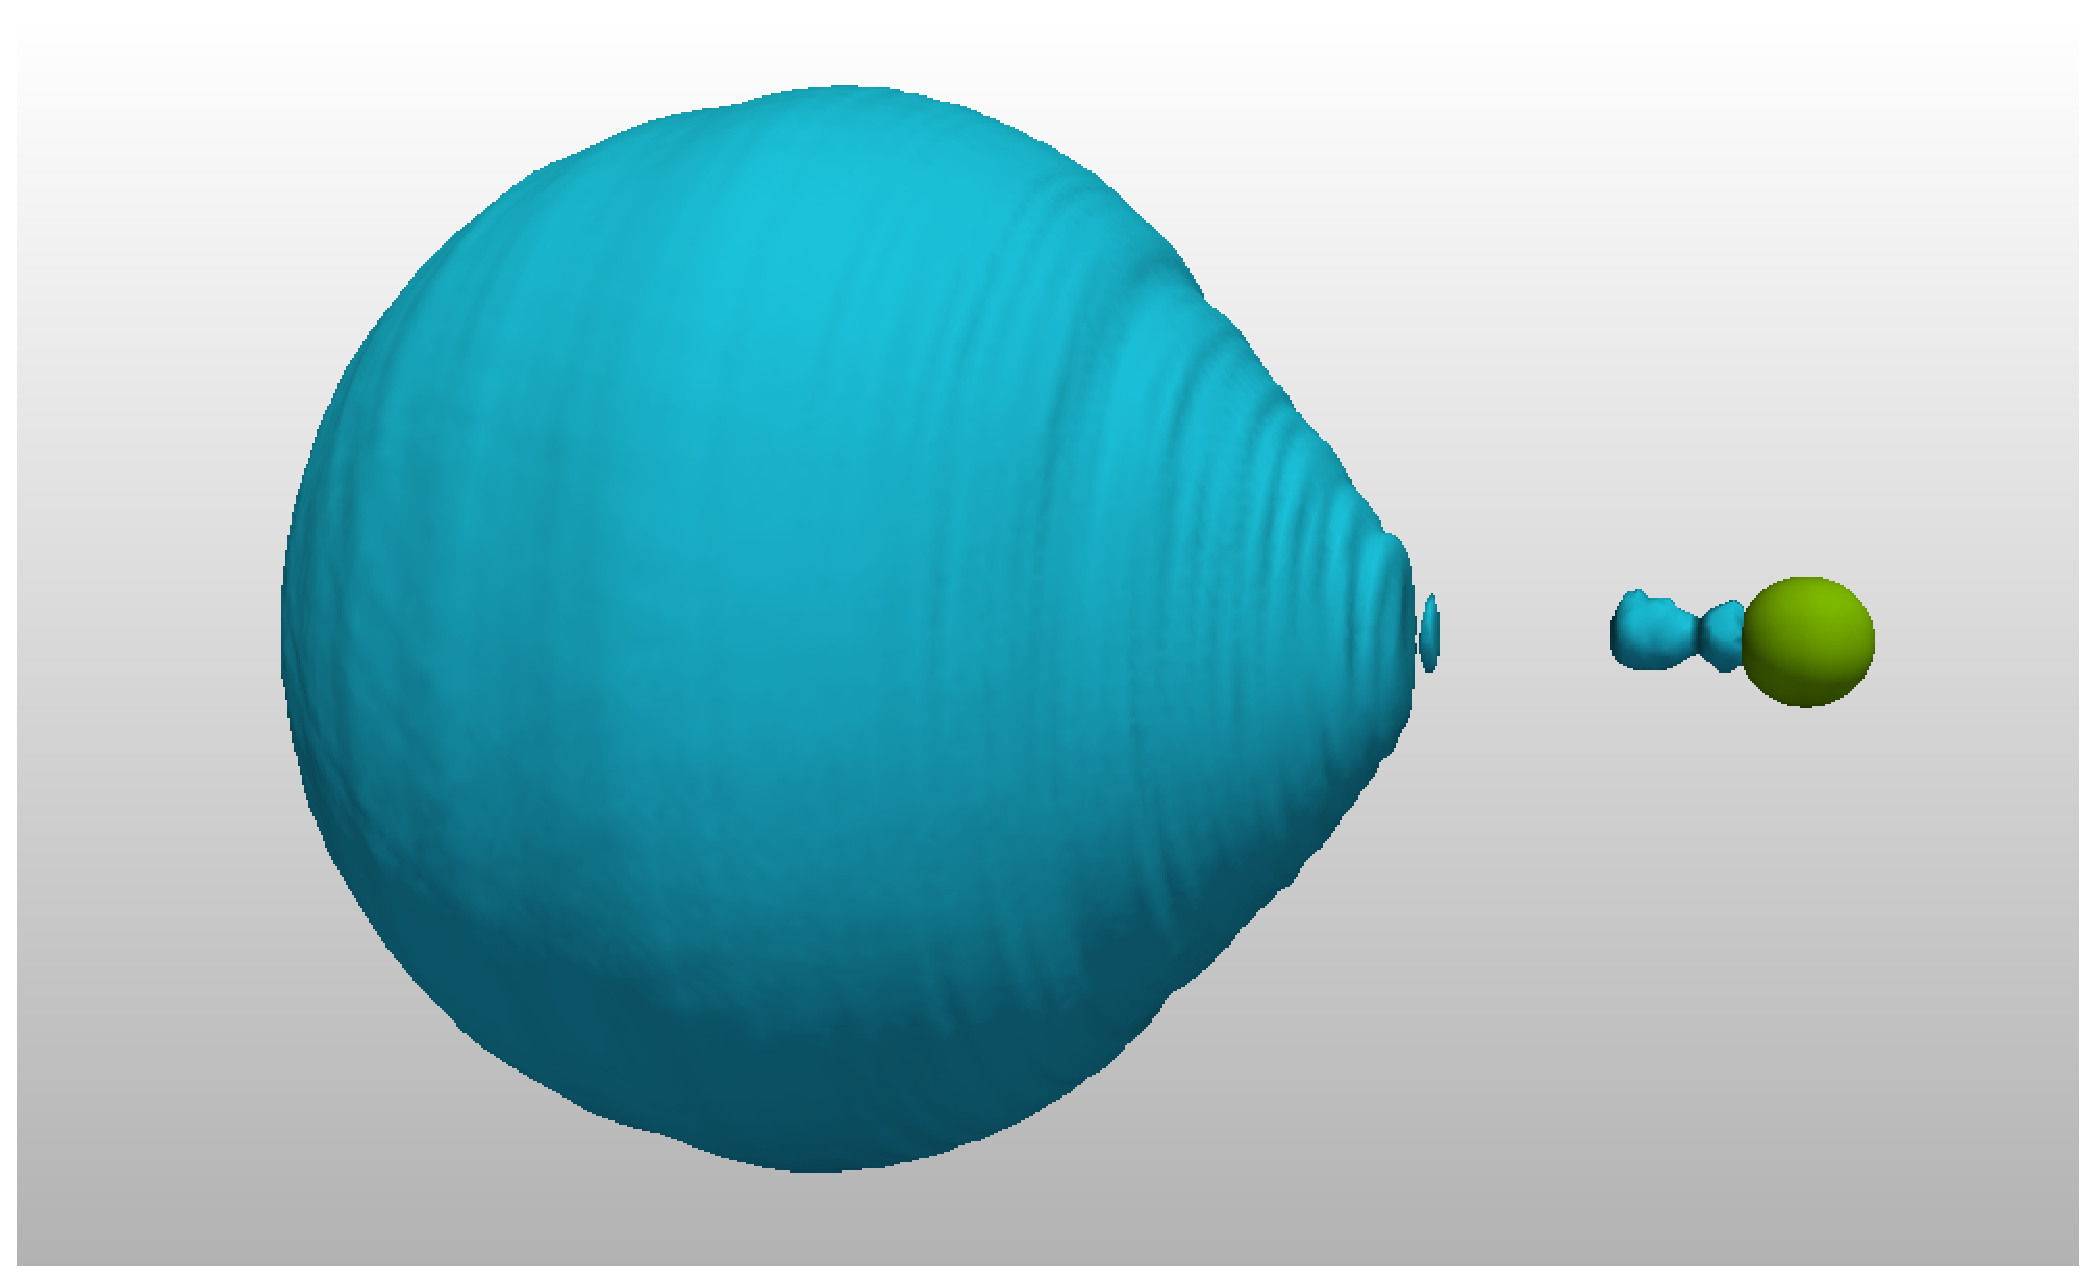
\includegraphics[scale=0.234]{4P-p32-fx-snap}}
		\caption{Snapshot of He$_N$ density with a linear KHe$_n$ exciplex leaving the droplet at $t=18.5$ ps\label{fig:4P-p32-fx-snap}}
	\end{minipage}
\hfill
	\begin{minipage}[c]{0.48\linewidth}
		% GNUPLOT: LaTeX picture with Postscript
\begingroup
  \makeatletter
  \providecommand\color[2][]{%
    \GenericError{(gnuplot) \space\space\space\@spaces}{%
      Package color not loaded in conjunction with
      terminal option `colourtext'%
    }{See the gnuplot documentation for explanation.%
    }{Either use 'blacktext' in gnuplot or load the package
      color.sty in LaTeX.}%
    \renewcommand\color[2][]{}%
  }%
  \providecommand\includegraphics[2][]{%
    \GenericError{(gnuplot) \space\space\space\@spaces}{%
      Package graphicx or graphics not loaded%
    }{See the gnuplot documentation for explanation.%
    }{The gnuplot epslatex terminal needs graphicx.sty or graphics.sty.}%
    \renewcommand\includegraphics[2][]{}%
  }%
  \providecommand\rotatebox[2]{#2}%
  \@ifundefined{ifGPcolor}{%
    \newif\ifGPcolor
    \GPcolortrue
  }{}%
  \@ifundefined{ifGPblacktext}{%
    \newif\ifGPblacktext
    \GPblacktextfalse
  }{}%
  % define a \g@addto@macro without @ in the name:
  \let\gplgaddtomacro\g@addto@macro
  % define empty templates for all commands taking text:
  \gdef\gplbacktext{}%
  \gdef\gplfronttext{}%
  \makeatother
  \ifGPblacktext
    % no textcolor at all
    \def\colorrgb#1{}%
    \def\colorgray#1{}%
  \else
    % gray or color?
    \ifGPcolor
      \def\colorrgb#1{\color[rgb]{#1}}%
      \def\colorgray#1{\color[gray]{#1}}%
      \expandafter\def\csname LTw\endcsname{\color{white}}%
      \expandafter\def\csname LTb\endcsname{\color{black}}%
      \expandafter\def\csname LTa\endcsname{\color{black}}%
      \expandafter\def\csname LT0\endcsname{\color[rgb]{1,0,0}}%
      \expandafter\def\csname LT1\endcsname{\color[rgb]{0,1,0}}%
      \expandafter\def\csname LT2\endcsname{\color[rgb]{0,0,1}}%
      \expandafter\def\csname LT3\endcsname{\color[rgb]{1,0,1}}%
      \expandafter\def\csname LT4\endcsname{\color[rgb]{0,1,1}}%
      \expandafter\def\csname LT5\endcsname{\color[rgb]{1,1,0}}%
      \expandafter\def\csname LT6\endcsname{\color[rgb]{0,0,0}}%
      \expandafter\def\csname LT7\endcsname{\color[rgb]{1,0.3,0}}%
      \expandafter\def\csname LT8\endcsname{\color[rgb]{0.5,0.5,0.5}}%
    \else
      % gray
      \def\colorrgb#1{\color{black}}%
      \def\colorgray#1{\color[gray]{#1}}%
      \expandafter\def\csname LTw\endcsname{\color{white}}%
      \expandafter\def\csname LTb\endcsname{\color{black}}%
      \expandafter\def\csname LTa\endcsname{\color{black}}%
      \expandafter\def\csname LT0\endcsname{\color{black}}%
      \expandafter\def\csname LT1\endcsname{\color{black}}%
      \expandafter\def\csname LT2\endcsname{\color{black}}%
      \expandafter\def\csname LT3\endcsname{\color{black}}%
      \expandafter\def\csname LT4\endcsname{\color{black}}%
      \expandafter\def\csname LT5\endcsname{\color{black}}%
      \expandafter\def\csname LT6\endcsname{\color{black}}%
      \expandafter\def\csname LT7\endcsname{\color{black}}%
      \expandafter\def\csname LT8\endcsname{\color{black}}%
    \fi
  \fi
    \setlength{\unitlength}{0.0500bp}%
    \ifx\gptboxheight\undefined%
      \newlength{\gptboxheight}%
      \newlength{\gptboxwidth}%
      \newsavebox{\gptboxtext}%
    \fi%
    \setlength{\fboxrule}{0.5pt}%
    \setlength{\fboxsep}{1pt}%
\begin{picture}(4752.00,2880.00)%
    \gplgaddtomacro\gplbacktext{%
      \csname LTb\endcsname%
      \put(682,432){\makebox(0,0)[r]{\strut{}$26$}}%
      \csname LTb\endcsname%
      \put(682,921){\makebox(0,0)[r]{\strut{}$27$}}%
      \csname LTb\endcsname%
      \put(682,1411){\makebox(0,0)[r]{\strut{}$28$}}%
      \csname LTb\endcsname%
      \put(682,1900){\makebox(0,0)[r]{\strut{}$29$}}%
      \csname LTb\endcsname%
      \put(682,2390){\makebox(0,0)[r]{\strut{}$30$}}%
      \csname LTb\endcsname%
      \put(682,2879){\makebox(0,0)[r]{\strut{}$31$}}%
      \csname LTb\endcsname%
      \put(814,212){\makebox(0,0){\strut{}$0$}}%
      \csname LTb\endcsname%
      \put(1554,212){\makebox(0,0){\strut{}$5$}}%
      \csname LTb\endcsname%
      \put(2294,212){\makebox(0,0){\strut{}$10$}}%
      \csname LTb\endcsname%
      \put(3033,212){\makebox(0,0){\strut{}$15$}}%
      \csname LTb\endcsname%
      \put(3773,212){\makebox(0,0){\strut{}$20$}}%
      \csname LTb\endcsname%
      \put(4513,212){\makebox(0,0){\strut{}$25$}}%
    }%
    \gplgaddtomacro\gplfronttext{%
      \csname LTb\endcsname%
      \put(176,1655){\rotatebox{-270}{\makebox(0,0){\strut{}K relative position (\AA)}}}%
      \put(2663,-74){\makebox(0,0){\strut{}Time (ps)}}%
      \csname LTb\endcsname%
      \put(3526,1765){\makebox(0,0)[r]{\strut{}Free}}%
      \csname LTb\endcsname%
      \put(3526,1545){\makebox(0,0)[r]{\strut{}Fixed}}%
    }%
    \gplbacktext
    \put(0,0){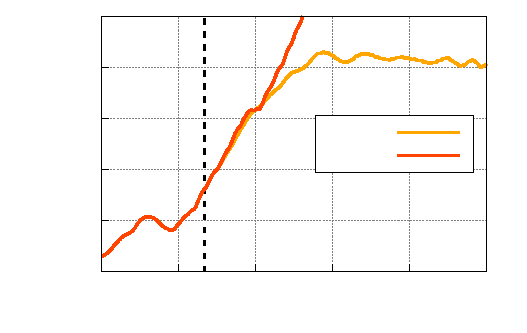
\includegraphics{4P-p32-fxd-pos}}%
    \gplfronttext
  \end{picture}%
\endgroup

		\vspace{0.2\baselineskip}
		\caption{Distance between K and He$_N$ centers of mass as a function of time, for fixed and free $\ket{\lambda}$\label{fig:4P-p32-fxd-pos}}
	\end{minipage}
\end{figure}

Comparing trajectories in the case of a free or fixed electronic state evolution (\citfig{fig:4P-p32-fxd-pos}) shows that the leaving exciplex seems to be the natural response of this system. 
Nevertheless when we let the internal state evolve, the system finds a way to handle a new symmetry which is the formation of a ring exciplex that is more cubic symmetry friendly.\\

We might be tempted to interpret these symmetry breakings as a possibility that could occur in a real experiment, due to spatial distortion of the droplet or any external perturbation. 
Hints for ring exciplex stability in the Cs case have been found \cite{Zbi2005}.
But this clearly remains an open question for potassium that requires further investigations.

\subsection{Comparison with exprimental data}

Alkali doped droplets have been studied extensively \cite{Sti1996,Lac2011,Lac2012,Bru2001,Her2012,Log2014,Log2015,Van2017}. 
Nevertheless there are only two articles that investigated the dynamics following $4p\leftarrow 4s$ excitation of a K-doped droplet: \cite{Reh2000A,Reh2000B} (single article split in two) and \cite{Sch2001}. 
\cite{Reh2000A,Reh2000B} collected dispersed emission spectra using reversed time-correlated single photon counting while \cite{Sch2001} used femtosecond pumb-probe spectroscopy. 
Both report the formation of exciplexes in the $\Pi$ states and desorption in the $\Sigma$ state. 
Both show that the most abundant product species is KHe.
They also report a $\sim$10\% KHe$_2$ production. \cite{Sch2001} even shows that KHe$_n$ exciplexes are formed with $n=3,4$ (2.3\% both) and $n=5$ (0.5\%). 
Nevertheless there is a huge discrepancy in the measured formation time scale. 
\cite{Reh2000A,Reh2000B} gives 50 $\pm$ 20 ps ($\Pi_{3/2}$) and 7.9 ns ($\Pi_{1/2}$),  whereas \cite{Sch2001} cannot resolve the two $\Pi$ states but gives 180 $\pm$ 60 fs (KHe) and 204$ \pm$ 60 fs (KHe$_2$).\\ 

After discussions with the authors of \cite{Sch2001} during a conference\footnote{Quantum Fluid Clusters conference, Obergurgl (Austria), June 7-9, 2017, where I presented a poster on my results}, it appears that their results on the time scale could be wrong due to a too high repetition rate of the exciting laser. 
They could have been exciting the $5p$ state (24701.382 cm$^{-1}$ and 24720.139 cm$^{-1}$ \cite{Nist}) trough a two-photon process. \\

We have seen that our simulation describes well the formation of exciplexes.
In particular the linear exciplex shape is consistent with the  K-He observed experimentally\footnote{He-TDDFT has been found to give non-integer numbers of atom in exciplexes, so we may only use qualitative arguments based on 3D representation} but no evidence for linear He-K-He (KHe$_2$) was found. The small proportion of higher $n$ exciplexes observed experimentally could be a hint for the existence of ring shaped configurations.\\

Concerning the time scale in our simulations, in $\Pi_{3/2}$ excitation the potassium trajectory shows that the exciplex starts to leave within 5 ps, the symmetry breaking occurs after the beginning of desorption. 
Fixing the electronic state demonstrates that this desorption is the physical answer of the system rather than bound configuration. 
In the $\Pi_{1/2}$ state we observe a bouncing free potassium (the simulation is still running but the time scale to reach a stationary state may be $\sim$ ns).
We could imagine that once in an equilibrium position, some tunneling effect may occur through the tiny barrier leading to exciplex formation within a few ns, see model presented in \cite{Reh2000A,Reh2000B}.
Finally, in the displaced $\Pi_{1/2}$ we cannot fix the internal state but during the formation of the linear exciplex the internal state goes to $\ket{p_1}$, which is the same than in $\Pi_{3/2}$.
This is why we can expect a departing exciplex (and not bound) within 15 ps.\\

These results are closer to the ones from \cite{Reh2000A,Reh2000B} which give 50 ps ($\Pi_{3/2}$) and 7.9 ns ($\Pi_{1/2}$) than \cite{Sch2001} which give 180 fs for both. 
This is probably explained by the setup dysfunctional described earlier.
The only true discrepancy that remains with \cite{Reh2000A,Reh2000B} is the $\Pi_{1/2}$ displaced excitation. We do not get a clear explanation, however as it is a turning point this could be a rare case in experiments. 
This could also be a limitation of our simulations.
\section{Excitation towards $5s$ state}

The last part of this study, which is still in progress, is the simulation of the $5s\leftarrow 4s$ photo-excitation. 
Since the ($5s$) state is isotropic, we could address this problem with both a classical and a quantum description for potassium.

\subsection{Qualitative behavior and time scale}

The first element that can be compared between the two approaches is the behavior of the potassium. 
In both cases it is ejected after excitation within 200 fs (\citfig{fig:5S-pos}). 
This was actually highly predictable looking at the pair potential (\citfig{fig:DIM-5s-pot}): it shows a potential energy of 700 K over the dissociation level (and in an isotropic state all helium-potassium pairs interact with the same potential). Nevertheless, we see that the asymptotic K velocity is not the same  in quantum and classical description (\citfig{fig:5S-vel}). We will investigate this point in the following paragraph.

\begin{figure}[h!]
	\centering
	\begin{minipage}[c]{0.48\linewidth}
		% GNUPLOT: LaTeX picture with Postscript
\begingroup
  \makeatletter
  \providecommand\color[2][]{%
    \GenericError{(gnuplot) \space\space\space\@spaces}{%
      Package color not loaded in conjunction with
      terminal option `colourtext'%
    }{See the gnuplot documentation for explanation.%
    }{Either use 'blacktext' in gnuplot or load the package
      color.sty in LaTeX.}%
    \renewcommand\color[2][]{}%
  }%
  \providecommand\includegraphics[2][]{%
    \GenericError{(gnuplot) \space\space\space\@spaces}{%
      Package graphicx or graphics not loaded%
    }{See the gnuplot documentation for explanation.%
    }{The gnuplot epslatex terminal needs graphicx.sty or graphics.sty.}%
    \renewcommand\includegraphics[2][]{}%
  }%
  \providecommand\rotatebox[2]{#2}%
  \@ifundefined{ifGPcolor}{%
    \newif\ifGPcolor
    \GPcolortrue
  }{}%
  \@ifundefined{ifGPblacktext}{%
    \newif\ifGPblacktext
    \GPblacktextfalse
  }{}%
  % define a \g@addto@macro without @ in the name:
  \let\gplgaddtomacro\g@addto@macro
  % define empty templates for all commands taking text:
  \gdef\gplbacktext{}%
  \gdef\gplfronttext{}%
  \makeatother
  \ifGPblacktext
    % no textcolor at all
    \def\colorrgb#1{}%
    \def\colorgray#1{}%
  \else
    % gray or color?
    \ifGPcolor
      \def\colorrgb#1{\color[rgb]{#1}}%
      \def\colorgray#1{\color[gray]{#1}}%
      \expandafter\def\csname LTw\endcsname{\color{white}}%
      \expandafter\def\csname LTb\endcsname{\color{black}}%
      \expandafter\def\csname LTa\endcsname{\color{black}}%
      \expandafter\def\csname LT0\endcsname{\color[rgb]{1,0,0}}%
      \expandafter\def\csname LT1\endcsname{\color[rgb]{0,1,0}}%
      \expandafter\def\csname LT2\endcsname{\color[rgb]{0,0,1}}%
      \expandafter\def\csname LT3\endcsname{\color[rgb]{1,0,1}}%
      \expandafter\def\csname LT4\endcsname{\color[rgb]{0,1,1}}%
      \expandafter\def\csname LT5\endcsname{\color[rgb]{1,1,0}}%
      \expandafter\def\csname LT6\endcsname{\color[rgb]{0,0,0}}%
      \expandafter\def\csname LT7\endcsname{\color[rgb]{1,0.3,0}}%
      \expandafter\def\csname LT8\endcsname{\color[rgb]{0.5,0.5,0.5}}%
    \else
      % gray
      \def\colorrgb#1{\color{black}}%
      \def\colorgray#1{\color[gray]{#1}}%
      \expandafter\def\csname LTw\endcsname{\color{white}}%
      \expandafter\def\csname LTb\endcsname{\color{black}}%
      \expandafter\def\csname LTa\endcsname{\color{black}}%
      \expandafter\def\csname LT0\endcsname{\color{black}}%
      \expandafter\def\csname LT1\endcsname{\color{black}}%
      \expandafter\def\csname LT2\endcsname{\color{black}}%
      \expandafter\def\csname LT3\endcsname{\color{black}}%
      \expandafter\def\csname LT4\endcsname{\color{black}}%
      \expandafter\def\csname LT5\endcsname{\color{black}}%
      \expandafter\def\csname LT6\endcsname{\color{black}}%
      \expandafter\def\csname LT7\endcsname{\color{black}}%
      \expandafter\def\csname LT8\endcsname{\color{black}}%
    \fi
  \fi
    \setlength{\unitlength}{0.0500bp}%
    \ifx\gptboxheight\undefined%
      \newlength{\gptboxheight}%
      \newlength{\gptboxwidth}%
      \newsavebox{\gptboxtext}%
    \fi%
    \setlength{\fboxrule}{0.5pt}%
    \setlength{\fboxsep}{1pt}%
\begin{picture}(4752.00,2880.00)%
    \gplgaddtomacro\gplbacktext{%
      \csname LTb\endcsname%
      \put(682,782){\makebox(0,0)[r]{\strut{}$26$}}%
      \csname LTb\endcsname%
      \put(682,1481){\makebox(0,0)[r]{\strut{}$27$}}%
      \csname LTb\endcsname%
      \put(682,2180){\makebox(0,0)[r]{\strut{}$28$}}%
      \csname LTb\endcsname%
      \put(682,2879){\makebox(0,0)[r]{\strut{}$29$}}%
      \csname LTb\endcsname%
      \put(814,212){\makebox(0,0){\strut{}$0$}}%
      \csname LTb\endcsname%
      \put(1554,212){\makebox(0,0){\strut{}$0.2$}}%
      \csname LTb\endcsname%
      \put(2294,212){\makebox(0,0){\strut{}$0.4$}}%
      \csname LTb\endcsname%
      \put(3033,212){\makebox(0,0){\strut{}$0.6$}}%
      \csname LTb\endcsname%
      \put(3773,212){\makebox(0,0){\strut{}$0.8$}}%
      \csname LTb\endcsname%
      \put(4513,212){\makebox(0,0){\strut{}$1$}}%
    }%
    \gplgaddtomacro\gplfronttext{%
      \csname LTb\endcsname%
      \put(176,1655){\rotatebox{-270}{\makebox(0,0){\strut{}K relative position (\AA)}}}%
      \put(2663,-74){\makebox(0,0){\strut{}Time (ps)}}%
      \csname LTb\endcsname%
      \put(3922,1031){\makebox(0,0)[r]{\strut{}Classical}}%
      \csname LTb\endcsname%
      \put(3922,811){\makebox(0,0)[r]{\strut{}Quantum}}%
    }%
    \gplbacktext
    \put(0,0){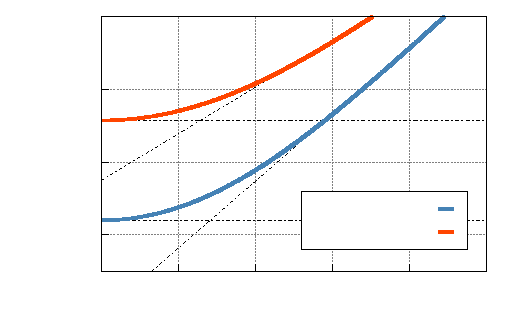
\includegraphics{5S-pos}}%
    \gplfronttext
  \end{picture}%
\endgroup

		\vspace{0.2\baselineskip}
		\caption{Distance between classical/quantum K and He$_N$ centers of mass as a function of time\label{fig:5S-pos}}
	\end{minipage}
\hfill
	\begin{minipage}[c]{0.48\linewidth}
		% GNUPLOT: LaTeX picture with Postscript
\begingroup
  \makeatletter
  \providecommand\color[2][]{%
    \GenericError{(gnuplot) \space\space\space\@spaces}{%
      Package color not loaded in conjunction with
      terminal option `colourtext'%
    }{See the gnuplot documentation for explanation.%
    }{Either use 'blacktext' in gnuplot or load the package
      color.sty in LaTeX.}%
    \renewcommand\color[2][]{}%
  }%
  \providecommand\includegraphics[2][]{%
    \GenericError{(gnuplot) \space\space\space\@spaces}{%
      Package graphicx or graphics not loaded%
    }{See the gnuplot documentation for explanation.%
    }{The gnuplot epslatex terminal needs graphicx.sty or graphics.sty.}%
    \renewcommand\includegraphics[2][]{}%
  }%
  \providecommand\rotatebox[2]{#2}%
  \@ifundefined{ifGPcolor}{%
    \newif\ifGPcolor
    \GPcolortrue
  }{}%
  \@ifundefined{ifGPblacktext}{%
    \newif\ifGPblacktext
    \GPblacktextfalse
  }{}%
  % define a \g@addto@macro without @ in the name:
  \let\gplgaddtomacro\g@addto@macro
  % define empty templates for all commands taking text:
  \gdef\gplbacktext{}%
  \gdef\gplfronttext{}%
  \makeatother
  \ifGPblacktext
    % no textcolor at all
    \def\colorrgb#1{}%
    \def\colorgray#1{}%
  \else
    % gray or color?
    \ifGPcolor
      \def\colorrgb#1{\color[rgb]{#1}}%
      \def\colorgray#1{\color[gray]{#1}}%
      \expandafter\def\csname LTw\endcsname{\color{white}}%
      \expandafter\def\csname LTb\endcsname{\color{black}}%
      \expandafter\def\csname LTa\endcsname{\color{black}}%
      \expandafter\def\csname LT0\endcsname{\color[rgb]{1,0,0}}%
      \expandafter\def\csname LT1\endcsname{\color[rgb]{0,1,0}}%
      \expandafter\def\csname LT2\endcsname{\color[rgb]{0,0,1}}%
      \expandafter\def\csname LT3\endcsname{\color[rgb]{1,0,1}}%
      \expandafter\def\csname LT4\endcsname{\color[rgb]{0,1,1}}%
      \expandafter\def\csname LT5\endcsname{\color[rgb]{1,1,0}}%
      \expandafter\def\csname LT6\endcsname{\color[rgb]{0,0,0}}%
      \expandafter\def\csname LT7\endcsname{\color[rgb]{1,0.3,0}}%
      \expandafter\def\csname LT8\endcsname{\color[rgb]{0.5,0.5,0.5}}%
    \else
      % gray
      \def\colorrgb#1{\color{black}}%
      \def\colorgray#1{\color[gray]{#1}}%
      \expandafter\def\csname LTw\endcsname{\color{white}}%
      \expandafter\def\csname LTb\endcsname{\color{black}}%
      \expandafter\def\csname LTa\endcsname{\color{black}}%
      \expandafter\def\csname LT0\endcsname{\color{black}}%
      \expandafter\def\csname LT1\endcsname{\color{black}}%
      \expandafter\def\csname LT2\endcsname{\color{black}}%
      \expandafter\def\csname LT3\endcsname{\color{black}}%
      \expandafter\def\csname LT4\endcsname{\color{black}}%
      \expandafter\def\csname LT5\endcsname{\color{black}}%
      \expandafter\def\csname LT6\endcsname{\color{black}}%
      \expandafter\def\csname LT7\endcsname{\color{black}}%
      \expandafter\def\csname LT8\endcsname{\color{black}}%
    \fi
  \fi
    \setlength{\unitlength}{0.0500bp}%
    \ifx\gptboxheight\undefined%
      \newlength{\gptboxheight}%
      \newlength{\gptboxwidth}%
      \newsavebox{\gptboxtext}%
    \fi%
    \setlength{\fboxrule}{0.5pt}%
    \setlength{\fboxsep}{1pt}%
\begin{picture}(4752.00,2880.00)%
    \gplgaddtomacro\gplbacktext{%
      \csname LTb\endcsname%
      \put(550,432){\makebox(0,0)[r]{\strut{}$0$}}%
      \csname LTb\endcsname%
      \put(550,840){\makebox(0,0)[r]{\strut{}$1$}}%
      \csname LTb\endcsname%
      \put(550,1248){\makebox(0,0)[r]{\strut{}$2$}}%
      \csname LTb\endcsname%
      \put(550,1656){\makebox(0,0)[r]{\strut{}$3$}}%
      \csname LTb\endcsname%
      \put(550,2063){\makebox(0,0)[r]{\strut{}$4$}}%
      \csname LTb\endcsname%
      \put(550,2471){\makebox(0,0)[r]{\strut{}$5$}}%
      \csname LTb\endcsname%
      \put(550,2879){\makebox(0,0)[r]{\strut{}$6$}}%
      \csname LTb\endcsname%
      \put(682,212){\makebox(0,0){\strut{}$0$}}%
      \csname LTb\endcsname%
      \put(1229,212){\makebox(0,0){\strut{}$2$}}%
      \csname LTb\endcsname%
      \put(1777,212){\makebox(0,0){\strut{}$4$}}%
      \csname LTb\endcsname%
      \put(2324,212){\makebox(0,0){\strut{}$6$}}%
      \csname LTb\endcsname%
      \put(2871,212){\makebox(0,0){\strut{}$8$}}%
      \csname LTb\endcsname%
      \put(3418,212){\makebox(0,0){\strut{}$10$}}%
      \csname LTb\endcsname%
      \put(3966,212){\makebox(0,0){\strut{}$12$}}%
      \csname LTb\endcsname%
      \put(4513,212){\makebox(0,0){\strut{}$14$}}%
    }%
    \gplgaddtomacro\gplfronttext{%
      \csname LTb\endcsname%
      \put(176,1655){\rotatebox{-270}{\makebox(0,0){\strut{}K velocity (\AA/ps)}}}%
      \put(2597,-74){\makebox(0,0){\strut{}Time (ps)}}%
      \csname LTb\endcsname%
      \put(3915,1031){\makebox(0,0)[r]{\strut{}Classical}}%
      \csname LTb\endcsname%
      \put(3915,811){\makebox(0,0)[r]{\strut{}Quantum}}%
    }%
    \gplbacktext
    \put(0,0){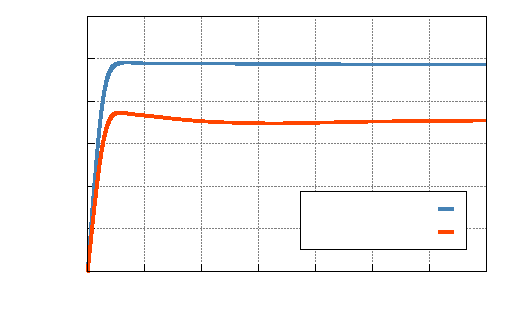
\includegraphics{5S-vel}}%
    \gplfronttext
  \end{picture}%
\endgroup

		\vspace{0.2\baselineskip}
		\caption{Velocity of classical/quantum K and He$_N$ as a function of time\newline{}\label{fig:5S-vel}}
	\end{minipage}
\end{figure}

\subsection{Strongly interacting neighbor helium atoms}

Let us consider a simple, impulsive  model, which has already been used in the past \cite{Her2012}. 
K interacts with $M$ neighboring He atoms. We assume that all the excitation energy $\Delta E$ (\textit{id est} excess energy with respect to the dissociation threshold) is converted into kinetic energy. 
We can write both energy and momentum conservation
\begin{align}
\frac{\vb{p}_\K^2}{2m\K}+\sum_\HE^M \cdot\frac{\vb{p}^2_{\HE}}{2m_\HE} &= \Delta E\\
\vb{p}_\K + \sum_\HE^M \cdot \vb{p}_\HE &= 0 
\end{align}
Then we make the following assumption: all He momentum are equal, this is quite a huge approximation but this model is simple. Then some basic algebra gives an expression for $M$
\begin{align}
\frac{\vb{p}_\K^2}{2m\K} &= \frac{M\cdot m_\HE}{m_K+M\cdot m_\HE} \Delta E \equiv \alpha \, \Delta E\\
M &= \frac{\alpha}{1-\alpha} \frac{m_\K}{m_\HE}
\end{align}

In order to probe different excitation energies we have to shift the initial position of the potassium at excitation time. 
In the classical description  of K we could study both diabatic or adiabatic helium density (\textit{with frozen or relaxed helium density for the new position)}, while the quantum case will only be discussed within the adiabatic approximation, but the diabatic one is being studied currently. 
\begin{figure}[h!]
\centering
\begin{minipage}[c]{0.48\linewidth}
\centering
		% GNUPLOT: LaTeX picture with Postscript
\begingroup
  \makeatletter
  \providecommand\color[2][]{%
    \GenericError{(gnuplot) \space\space\space\@spaces}{%
      Package color not loaded in conjunction with
      terminal option `colourtext'%
    }{See the gnuplot documentation for explanation.%
    }{Either use 'blacktext' in gnuplot or load the package
      color.sty in LaTeX.}%
    \renewcommand\color[2][]{}%
  }%
  \providecommand\includegraphics[2][]{%
    \GenericError{(gnuplot) \space\space\space\@spaces}{%
      Package graphicx or graphics not loaded%
    }{See the gnuplot documentation for explanation.%
    }{The gnuplot epslatex terminal needs graphicx.sty or graphics.sty.}%
    \renewcommand\includegraphics[2][]{}%
  }%
  \providecommand\rotatebox[2]{#2}%
  \@ifundefined{ifGPcolor}{%
    \newif\ifGPcolor
    \GPcolortrue
  }{}%
  \@ifundefined{ifGPblacktext}{%
    \newif\ifGPblacktext
    \GPblacktextfalse
  }{}%
  % define a \g@addto@macro without @ in the name:
  \let\gplgaddtomacro\g@addto@macro
  % define empty templates for all commands taking text:
  \gdef\gplbacktext{}%
  \gdef\gplfronttext{}%
  \makeatother
  \ifGPblacktext
    % no textcolor at all
    \def\colorrgb#1{}%
    \def\colorgray#1{}%
  \else
    % gray or color?
    \ifGPcolor
      \def\colorrgb#1{\color[rgb]{#1}}%
      \def\colorgray#1{\color[gray]{#1}}%
      \expandafter\def\csname LTw\endcsname{\color{white}}%
      \expandafter\def\csname LTb\endcsname{\color{black}}%
      \expandafter\def\csname LTa\endcsname{\color{black}}%
      \expandafter\def\csname LT0\endcsname{\color[rgb]{1,0,0}}%
      \expandafter\def\csname LT1\endcsname{\color[rgb]{0,1,0}}%
      \expandafter\def\csname LT2\endcsname{\color[rgb]{0,0,1}}%
      \expandafter\def\csname LT3\endcsname{\color[rgb]{1,0,1}}%
      \expandafter\def\csname LT4\endcsname{\color[rgb]{0,1,1}}%
      \expandafter\def\csname LT5\endcsname{\color[rgb]{1,1,0}}%
      \expandafter\def\csname LT6\endcsname{\color[rgb]{0,0,0}}%
      \expandafter\def\csname LT7\endcsname{\color[rgb]{1,0.3,0}}%
      \expandafter\def\csname LT8\endcsname{\color[rgb]{0.5,0.5,0.5}}%
    \else
      % gray
      \def\colorrgb#1{\color{black}}%
      \def\colorgray#1{\color[gray]{#1}}%
      \expandafter\def\csname LTw\endcsname{\color{white}}%
      \expandafter\def\csname LTb\endcsname{\color{black}}%
      \expandafter\def\csname LTa\endcsname{\color{black}}%
      \expandafter\def\csname LT0\endcsname{\color{black}}%
      \expandafter\def\csname LT1\endcsname{\color{black}}%
      \expandafter\def\csname LT2\endcsname{\color{black}}%
      \expandafter\def\csname LT3\endcsname{\color{black}}%
      \expandafter\def\csname LT4\endcsname{\color{black}}%
      \expandafter\def\csname LT5\endcsname{\color{black}}%
      \expandafter\def\csname LT6\endcsname{\color{black}}%
      \expandafter\def\csname LT7\endcsname{\color{black}}%
      \expandafter\def\csname LT8\endcsname{\color{black}}%
    \fi
  \fi
    \setlength{\unitlength}{0.0500bp}%
    \ifx\gptboxheight\undefined%
      \newlength{\gptboxheight}%
      \newlength{\gptboxwidth}%
      \newsavebox{\gptboxtext}%
    \fi%
    \setlength{\fboxrule}{0.5pt}%
    \setlength{\fboxsep}{1pt}%
\begin{picture}(4752.00,2880.00)%
    \gplgaddtomacro\gplbacktext{%
      \csname LTb\endcsname%
      \put(814,432){\makebox(0,0)[r]{\strut{}$0$}}%
      \csname LTb\endcsname%
      \put(814,1044){\makebox(0,0)[r]{\strut{}$200$}}%
      \csname LTb\endcsname%
      \put(814,1656){\makebox(0,0)[r]{\strut{}$400$}}%
      \csname LTb\endcsname%
      \put(814,2267){\makebox(0,0)[r]{\strut{}$600$}}%
      \csname LTb\endcsname%
      \put(814,2879){\makebox(0,0)[r]{\strut{}$800$}}%
      \csname LTb\endcsname%
      \put(946,212){\makebox(0,0){\strut{}$0$}}%
      \csname LTb\endcsname%
      \put(1838,212){\makebox(0,0){\strut{}$500$}}%
      \csname LTb\endcsname%
      \put(2730,212){\makebox(0,0){\strut{}$1000$}}%
      \csname LTb\endcsname%
      \put(3621,212){\makebox(0,0){\strut{}$1500$}}%
      \csname LTb\endcsname%
      \put(4513,212){\makebox(0,0){\strut{}$2000$}}%
    }%
    \gplgaddtomacro\gplfronttext{%
      \csname LTb\endcsname%
      \put(176,1655){\rotatebox{-270}{\makebox(0,0){\strut{}Kinetik energy (K)}}}%
      \put(2729,-118){\makebox(0,0){\strut{}Excitation energy (K)}}%
      \csname LTb\endcsname%
      \put(2266,2651){\makebox(0,0)[r]{\strut{}Quantum}}%
      \csname LTb\endcsname%
      \put(2266,2431){\makebox(0,0)[r]{\strut{}Adiabatic}}%
      \csname LTb\endcsname%
      \put(2266,2211){\makebox(0,0)[r]{\strut{}Diabatic}}%
    }%
    \gplbacktext
    \put(0,0){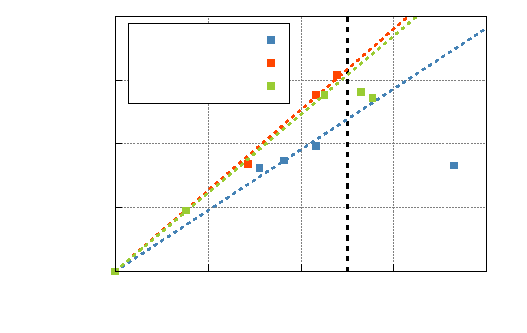
\includegraphics{5S-mass}}%
    \gplfronttext
  \end{picture}%
\endgroup

\end{minipage}
\hfill
\begin{minipage}[c]{0.48\linewidth}
\centering
\begin{tabular}{|c|c|c|c|}
\hline
K motion & Quantum	& \multicolumn{2}{c|}{Classical} \\
\hline
He density & Adiabatic	& Adiabatic & Diabatic \\
  \hline
	$\alpha$ & 0.38 & 0.50 & 0.49 \\
	\hline
	$M$ & 6.03 & 10.06 & 9.49 \\
  \hline
\end{tabular}
\end{minipage}
\vspace{0.5\baselineskip}
		\caption{Asymptotic kinetic energy as a function of excitation energy, comparison between diabatic/adiabatic classical and quantum description, and table of values for linear fit\label{fig:5S-mass}}
\end{figure}

Our model seems to work well up to 1250 K then we see some non linear effects. It is presumably due to a large amount of energy exchange with the droplet, which can no longer be described as impulsive, hard-sphere like dissociation.
We note that the classical description of K gives a higher number of neighboring helium atoms than the quantum one.
This can be surprising at first, but if we look at the ground state density profile (\citfig{fig:4S-Q-C-lsolid}), we note that the edge is smoother, so the density of neighboring atoms is lower. 
Nevertheless we are still investigating this point. 
Finally, adiabatic and diabatic descriptions seem to give similar results in classical case. 
This means that changes in density imposed by K fluctuation in equilibrium state has more or less no consequence on final kinetic energy, which is not really surprising as we are looking for asymptotic value.




\newpage\null\thispagestyle{empty}\newpage

% = CONCLUSION ============================= %
\chapter*{Conclusion}
\addcontentsline{toc}{chapter}{Conclusion}

The first goal of this study was to investigate the $4p \leftarrow 4s$ photo-excitation of a potassium doping a droplet in order to compare with experiments. 
We have shown that the qualitative behavior reported in both references \cite{Reh2000A,Reh2000B,Sch2001} was well described by our simulations.
In particularly, the formation of exciplexes was observed in $\Pi$ states and the ejection of a bare potassium atom in the $\Sigma$ state. 
We noted that the spatial resolution and the cubic grid were not optimal to describe the cylindrical symmetry underlying exciplexes formation.
This is why we only could make weak conclusions regarding the time scale, size and shape of exciplexes. 
Nevertheless, our results concerning their formation rate are clearly more consistent with \cite{Reh2000A,Reh2000B}.
This conclusion has been corroborated in a direct exchange with the authors of \cite{Sch2001}.
They told us that they could have failed in properly time-resolving the excitation dynamics because of the high repetition rate of their laser at the time. 
Finally, both references observed a dominant production of K$^*$He exciplexes and a significant proportion (10 \%) of K$^*$He$_2$ (and even larger exciplexes for \cite{Sch2001}), while our simulations tend to show only K-He exciplex (before symmetry breaking). 
The physical relevance of ring exciplex formation after symmetry breaking is not clear and need to be clarified.\\

The second point that is still under investigation at the moment, is the $5s \leftarrow 4s$ photo-excitation. 
There is no experimental literature on this transition, this study is then purely predictive. 
We have performed two different simulations, one with the potassium atom treated as a classical and one as a quantum particle.
 We observed that the potassium behavior is the same in both descriptions: it is ejected quickly from the droplet within 0.2 ps. 
 Nevertheless the asymptotic velocity is not the same.
This is why we focused our comparison on the study of an impulsive model giving an estimate of the number of closest atoms directly interacting with the potassium at the time of photoexcitation. 
We have shown that the quantum case gave a lower number than the classical one, which explains that there is less momentum given to K.\\

To conclude, this work demonstrates once again that He-TDDFT coupled with DIM model is a very powerful tool to address the dynamics of helium droplets doped by an alkali atom upon photo-excitation. 
We could give a theoretical contribution to choose between the two contradictory experimental results. 
However, we also underlined difficulty of the 4HeDFT-BCN-TLS code in describing exciplex formation due to a simulation grid unadapted to the cylindrical symmetry at small scale. 
Finally, we started to describe the potassium desorption upon excitation to the $5s$ state. 
We hope that our results will motivate experimentalists to work on both transitions.\\ 

In a close future, we would like to study the $4p \leftarrow 4s$ transition with test particles in order to evaluate the importance of quantum effects in this case.
We also want to address the question of the formation of a ring exciplex, and to finish our study of the $5s \leftarrow 4s$ transition. 
A long term motivation could be to rewrite part of the code to bypass the cubic limitation and get better results.



\newpage\null\thispagestyle{empty}\newpage

% = ANNEXES ================================ %
\chapter*{Annex: technical details on coding}
\addcontentsline{toc}{chapter}{Annexe: technical details on coding}

\setcounter{table}{0}
\setcounter{section}{0}
\renewcommand{\thetable}{\arabic{table}}
\renewcommand{\thechapter}{}
\renewcommand{\thesection}{\alph{section}}

\label{sec:ANX}
The code we used is the 4He-DFT BCN-TLS \cite{BCNcode}.
A detailed description is provided in \cite{DFTguide}. 
We give here the most important features about the computational approach. 
Equations are solved on a real space cubic grid.
In order to compute the convolution products involved in the functional, we also work in \textsc{Fourier}'s space, which is why we use a cubic mesh. 

\section{Imaginary time propagation}
\label{sec:ANX-itp}

In order to find ground state properties we have to minimize a \textsc{Schrödinger}-like equation. 
Let us consider that we know the eigenvectors $\{\phi_k\}$ of the given Hamiltonian with energies $\{\varepsilon_k\}$
\begin{align}
H \phi_k = \varepsilon_k \phi_k 
\end{align}

Since $H$ does not depend on time, one can formally write the propagation in time of a given $\psi$ as
\begin{align}
\label{eq:ITP}
i\hbar \pdv{t} \psi &= H\psi \Rightarrow \psi(t) = \e^{-i\frac{t}{\hbar} H} \, \psi(0)
\end{align}

Let us now introduce an \textit{imaginary time} as $\tau = i t/\hbar$ and rewrite (\citeq{eq:ITP}) as a function of $\tau$
\begin{align}
i\hbar \pdv{\tau} \dv{\tau}{t} \psi &= H \psi \Rightarrow \pdv{\tau} \psi = - H \psi \Rightarrow \psi(\tau) = \e^{- \tau H } \, \psi(0)
\end{align}

We expand $\psi(0)$ in the basis $H$ eigenvectors
\begin{align}
\psi(0) = \sum_{k=0}^{k=\infty} \alpha_k \phi_k \quad \text{and} \quad H \phi_k = \varepsilon_k \phi_k \Rightarrow \psi(\tau) = \sum_{k=0}^{k=\infty} \alpha_k \, \e^{-\tau \varepsilon_k }  \, \phi_k 
\label{eq:ITP-dead}
\end{align}

What we see in \citeq{eq:ITP-dead}, is that upon propagation with  imaginary time, only the ground state survives. In practice to compute $\psi(\tau)$ we use 
\begin{align}
\psi(\tau+\delta \tau) \approx (1-\delta \tau H) \, \psi(\tau) \equiv \psi(\tau) + \delta \psi(\tau)
\end{align}

This expression is iterated until convergence, which gives the ground state eigenvector and  its associated eigenvalue
\begin{align}
\varepsilon_0 = \frac{\bra{\Psi}H\ket{\Psi}}{\braket{\Psi}{\Psi}}
\end{align}



\section{Real time propagation}
\label{sec:ANX-rtp}

To solve time dependent equations we use \textsc{Hamming}'s predictor-modifier-corrector method which is detailed in \cite{B-Ral1960}. Let us consider a system of $N$ ordinary differential equations
\begin{align}
\dot{\vb{y}} \equiv \dv{\vb{y}}{x}=\vb{f}(x,\vb{y}) \with \vb{f}:\mathbb{R}^{N+1}\rightarrow\mathbb{R}^N \quad \text{and} \quad \vb{y} \in \mathbb{R}^N
\end{align}
We set $\vb{y}(x_0) = \vb{y}_0$ and we denote by $h$ the $x$ step. Higher order differential equations can be reduced to a system of coupled differential equations. We apply the following scheme whose error is $\mathcal{O}(h^5)$
\begin{align}
&\text{[Predictor]} \quad \vb{p}_{n+1} =\vb{y}_{n-3} + \frac{4h}{3}(2\dot{\vb{y}}_n-\dot{\vb{y}}_{n-1} + 2\dot{\vb{y}}_{n-2}) \label{eq:RTP-3} \\
&\text{[Modifier]} \quad \vb{m}_{n+1} = \vb{p}_{n+1} - \frac{112}{121}(\vb{p}_n-\vb{c}_n) \quad \text{and} \quad \dot{\vb{m}}_{n+1} =\vb{f}(x_{n+1},\vb{m}_{n+1}) \\
&\text{[Corrector]} \quad \vb{c}_{n+1} = \frac{1}{8}(9\vb{y}_n-\vb{y}_{n-2}+3h(\dot{\vb{m}}_{n+1} + 2 \dot{\vb{y}}_n-\dot{\vb{y}}_{n-1})) \\
&\text{[Final value]} \quad \vb{y}_{n+1} = \vb{c}_{n+1} + \frac{9}{121}(\vb{p}_{n+1}-\vb{c}_{n+1})
\end{align}

The main advantage of this algorithm is that it only requires two evaluations of $\vb{f}$ per step and this is the time consuming part of our calculation. 
Nevertheless note that is a not a self starting method, it requires values from three preceding steps (see \citeq{eq:RTP-3}). We need to be at least as accurate than $\mathcal{O}(h^5)$ this is why we initialize the computation by using \textsc{Runge-Kutta-Gill} method
\begin{align}
\vb{k}_1 &= h \, \vb{f} ( x_n,y_n) \\
\vb{k}_2 &= h \, \vb{f}\left(x_n+\frac{h}{2}, \vb{y}_n + \frac{1}{2}\,\vb{k}_1  \right)\\
\vb{k}_3 &= h \, \vb{f}\left(x_n+\frac{h}{2}, \vb{y}_n + (-1+\sqrt{2}) _, \vb{k}_1 + \left(1-\frac{\sqrt{2}}{2}\right)\vb{k}_2\right)\\
\vb{k}_4 &= h \, \vb{f}\left(x_n+h, \vb{y}_n -\frac{\sqrt{2}}{2} \, \vb{k}_2 + \left(1+\frac{\sqrt{2}}{2}\right)\vb{k}_3\right)\\
\vb{y}_{n+1} &= \vb{y}_n + \frac{1}{6} \left(\vb{k}_1 + (2-\sqrt{2}) \, \vb{k}_2 + (2+\sqrt{2}) \, \vb{k}_3 + \vb{k}_4\right) + \mathcal{O}(h^5)
\end{align}

We do not discuss here the boundary conditions, in particular how we can deal with helium leaving the droplet, because it is beyond the scope of this annex, this is explained in details in \cite{DFTguide}.
\section{Simulating spectra}
\label{sec:ANX-spectra}

The width of absorption spectrum is the result of helium density and potassium wave function fluctuations. In order to simulate this spectrum, we use the DF sampling method, the interested reader should refer to \cite{Mat2011}.\\

One can write, using the time dependent formulation, that within the \textsc{Born-Oppenheimer} approximation, the intensity associated with an electronic transition from a state $i$ to a state $f$ writes as
\begin{align}
I(\omega)\propto \int \dd{t} \e^{i(\omega+\omega_i)t} \int \dd{\vb{r}} (\mu_{f\leftarrow i}\, \phi_i)^* \, \e^{-iH_f t/\hbar}  \, (\mu_{f\leftarrow i} \, \phi_i)
\end{align}

In this expression $\phi_i$ refers to the eigenfunction of potassium in the initial state with energy $\hbar \omega_i$, $\mu_{f\leftarrow i}$ is the electronic transition dipole and $H_f$ is the potassium Hamiltonian in the final state that can written as a sum of kinetic and potential energy $H=T+V(\vb{r}_\K)$.\\

We can then expand $\phi$ in a basis of eigenvectors $\alpha_\nu(\vb{r}) $ $H_f$, which  gives an expression for the intensity
\begin{align}
\phi(\vb{r})&=\sum_\nu a_\nu \alpha_\nu(\vb{r}) \with a_\nu = \int \dd{\vb{r}} \alpha_\nu^*(\vb{r}) \phi_i(\vb{r})\\
I(\omega)&=\sum_\nu |a_\nu|^2 \, \delta(\omega-(\omega_\nu-\omega_i))
\end{align}

This gives a spectrum of lines with energies $\hbar(\omega_\nu-\omega_i)$ and relative intensities $|a_\nu|^2$ which are the so-called \textsc{Franck-Condon} factors . Considering that the final states are a quasi-continuous spectrum of $H_f$, it can be assumed that kinetic contribution is negligible. 
Then we can integrate over time and we obtain the semi-classical expression for the intensity, which is often called \textit{reflection principle}.
\begin{align}
I(\omega)=\int \dd{\vb{r}} |\phi_i(\vb{r})|^2 \, \delta \left(\omega-\left(\frac{V(\vb{r})}{\hbar} - \omega_i\right)\right) 
\end{align}

In order to evaluate this expression, we randomly generate $n_c$ configuration of $N$ positions for the helium atoms and one for potassium. 
The helium positions are generated from the converged density with a hard-sphere repulsion (exclusion volume with radius 2.18 \AA{}) which is supposed to represent the He-He correlation (one may actually refer to \cite{DFTguide} because the radius of exclusion is chosen density-dependent, but this is beyond the scope of this simple explanation). 
The potassium position can be either generated from its wave function in a quantum treatment or from its classical position. For a given sampled configuration $\{k\}$ the transition energy is
\begin{align}
E\{k\}=V_f\{k\}-V_i\{k\}
\end{align}
where $V$ corresponds to a sum over pair interactions which is written as $E^{nl}_{ij\alpha\beta}$ in \citeq{eq:DIM-defE} with $\{nl,i,j,\alpha,\beta\}$ fixed by the state we are interested in. 
Finally we get the spectrum by collecting each configuration contribution in a histogram.
\begin{align}
I(\omega)\propto \frac{1}{n_c} \sum_{\{k\}} \delta \left(\omega-\frac{E\{k\}}{\hbar}\right) 
\end{align}


\section{Values of functional parameters}
\label{sec:ANX-values}
\renewcommand{\arraystretch}{1.0} 
\newcolumntype{A}{>{\centering\arraybackslash}p{0.15\textwidth}}
\newcolumntype{B}{>{\centering\arraybackslash}X}
\newcolumntype{C}{>{\centering\arraybackslash}p{0.35\textwidth}}
\begin{table}[!h]
\centering
	\begin{minipage}[c]{0.48\linewidth}
	\centering
\begin{tabularx}{0.85\textwidth}{|A|B|C|}
\hline
Name & Units & Value \\
\hline
$\varepsilon_\LJ $ & K & 10.22 \\
$\sigma$ & \AA & 2.556 \\
\hline
$h$ & \AA & 2.190323 \\
$c_2$ & K\AA$^6$ & -2.41186$\times10^4$  \\
$c_3$ & K\AA$^9$ &  1.85850$\times10^6$ \\
\hline
$\alpha_s$ & \AA$^3$  & 54.31 \\
$\rho_0$ & \AA$^{-3}$ & 0.04  \\
$l$ & \AA & 1.0 \\
\hline
\end{tabularx}
	\end{minipage}
\hfill
	\begin{minipage}[c]{0.48\linewidth}
	\centering
\begin{tabularx}{0.85\textwidth}{|A|B|C|}
\hline
$C$ & Hartree & 0.1 \\
$\beta$ & \AA$^3$ & 40.0  \\
$\rho_m$ & \AA$^{-3}$ & 0.37 \\
\hline
$\gamma_{11}$ & & -19.7544 \\
$\gamma_{12}$ & \AA$^{-2}$ & 15.5616 \\
$\alpha_1$ & \AA$^{-2}$ & 1.023 \\
$\gamma_{21}$ & & -0.2395 \\
$\gamma_{22}$ & \AA$^{-2}$ & 0.0312 \\
$\alpha_2$ & \AA$^{-2}$ & 0.14912 \\
\hline
\end{tabularx}
	\end{minipage}
\caption{Parameters value of the different functional}
\label{tab:ANX-values}
\end{table}

\newpage\null\thispagestyle{empty}\newpage

% = BIBLIO ================================= %
\addcontentsline{toc}{chapter}{Bibliography}
\begingroup
\raggedright
\sloppy
\printbibliography
\endgroup

\end{document} 
